\chapter{Results and Discussion}

\section{Phase One : Imitation Learning}

\subsection{Single trajectory}

Initially, the policy was trained on a single trajectory. The goal was just 
to test whether it will be able to learn to overfit this single trajectory or
no. If it is not able to, then there is no reason to attempt to generalize
and the observation space, network architecture ...etc needs to be revised. If
it is able to learn the single trajectory, then we can proceed with the 
generalization and train on multiple trajectories. Many solutions were
tested in this phase until a working one was reached (that was discussed in 
the Methodology chapter). 

\noindent\textbf{Reference trajectory}

The load reference trajectory, i.e.\ the goal of the whole system, is a
straight move of 11\,m along the $x$-axis over 25\,s, with no motion along
the $y$ and $z$ axes. The load is static at the beginning and at the end,
and moves at a constant velocity of 1.1\,m/s for 10\,s in between. This
trajectory was chosen to engage the optimizer and force it to change $A$
and $\xi$ mid-trajectory.

\begin{figure}[H]
  \centering
  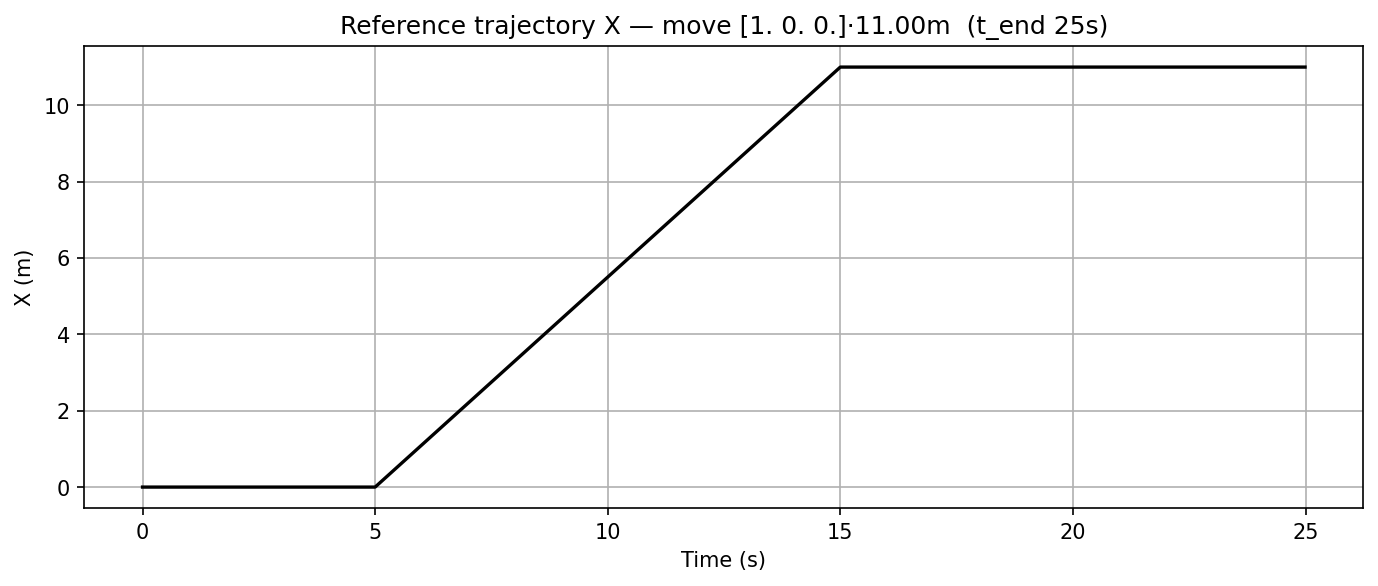
\includegraphics[width=0.8\textwidth]{figures/fig-reference-trajectory-x.png}
  \caption{Load reference trajectory along the $x$-axis ($t_{end}=25$\,s).}
  \label{fig:reference-trajectory-x}
\end{figure}

\noindent\textbf{Expert behavior}

The figures below show the Classical Control Stack (CCS - the expert 
using the original optimizer) behavior on the reference
trajectory: a 11\,m move along the $x$-axis over 25\,s. This behavior serves
as the reference that the proposed imitation learning (IL) policy aims to 
imitate. These figures were obtained by implementing the methodology 
presented in [5] and are shown here to provide the reader with a 
reference for the behavior being imitated.


\begin{figure}[H]
  \centering
  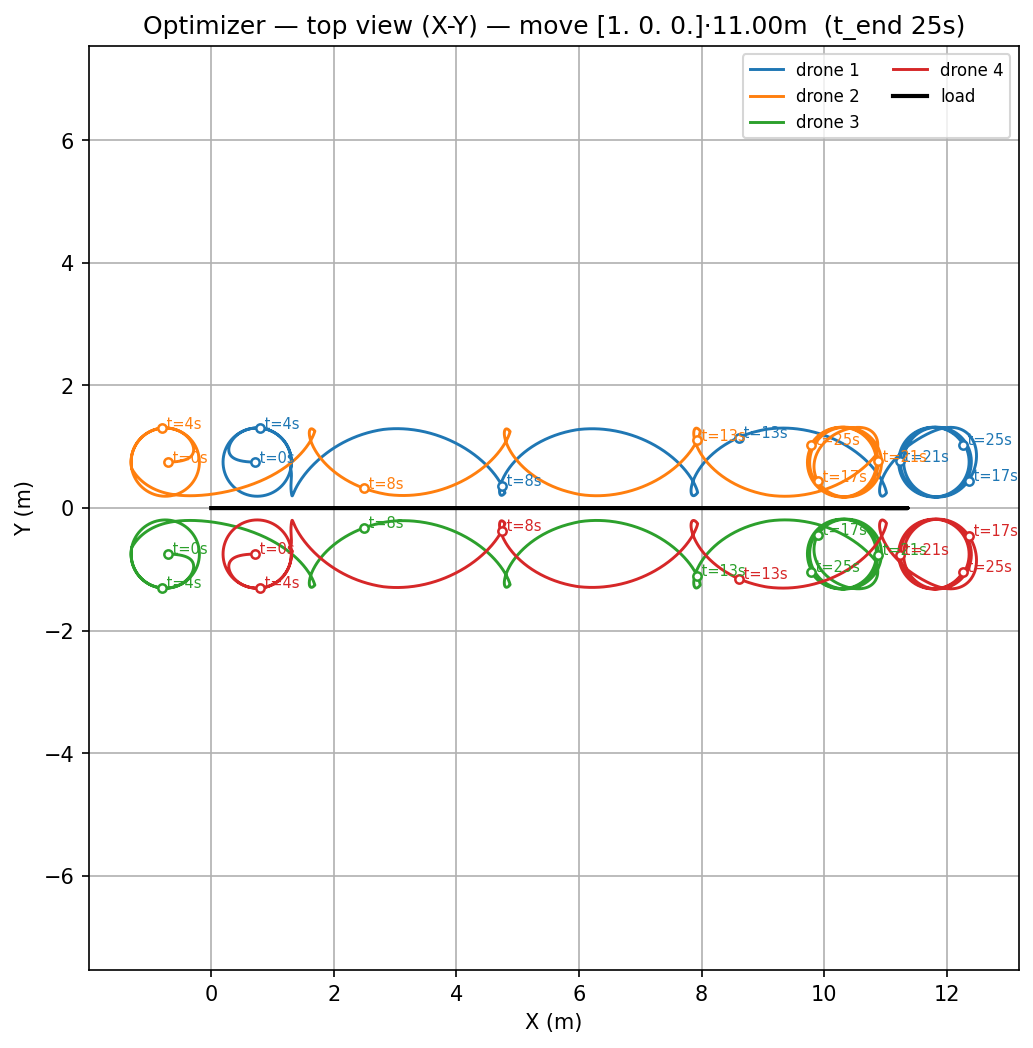
\includegraphics[width=0.6\textwidth]{figures/fig-expert-topview.png}
  \caption{CCS carrier and load trajectories top view (X-Y) for a move of 11\,m along $x$ ($t_{end}=25$\,s).}
  \label{fig:expert-topview}
\end{figure}

\begin{figure}[H]
  \centering
  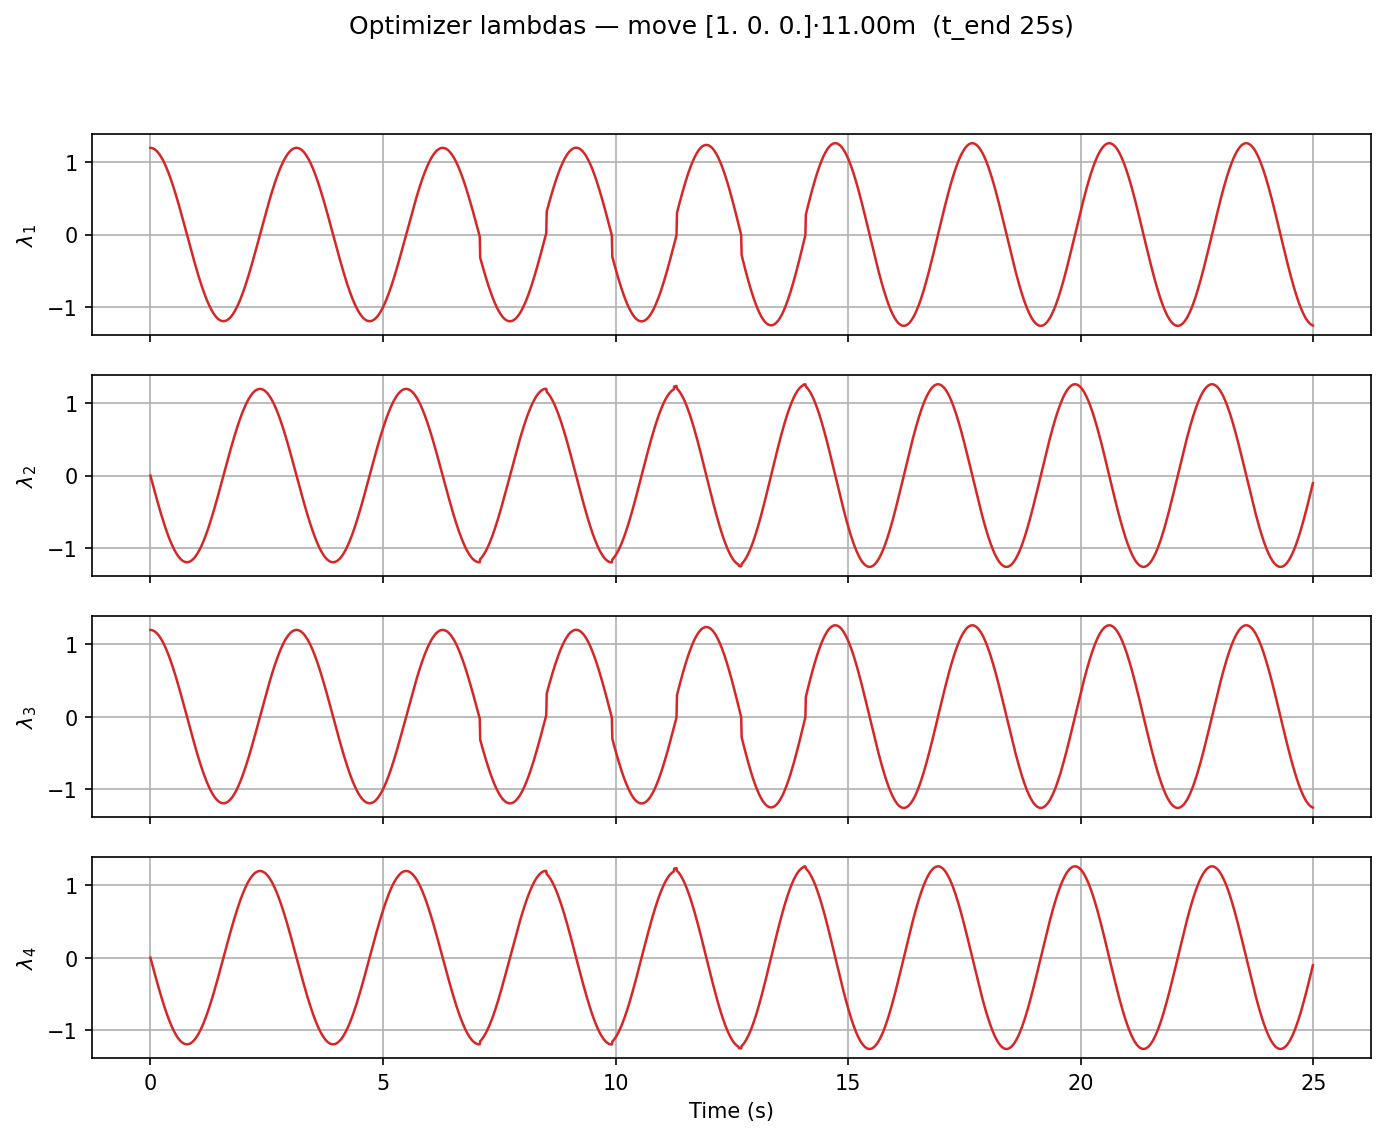
\includegraphics[width=0.8\textwidth]{figures/fig-expert-lambdas.png}
  \caption{Optimizer $\lambda$ values for the same trajectory.}
  \label{fig:expert-lambdas}
\end{figure}

\begin{figure}[H]
  \centering
  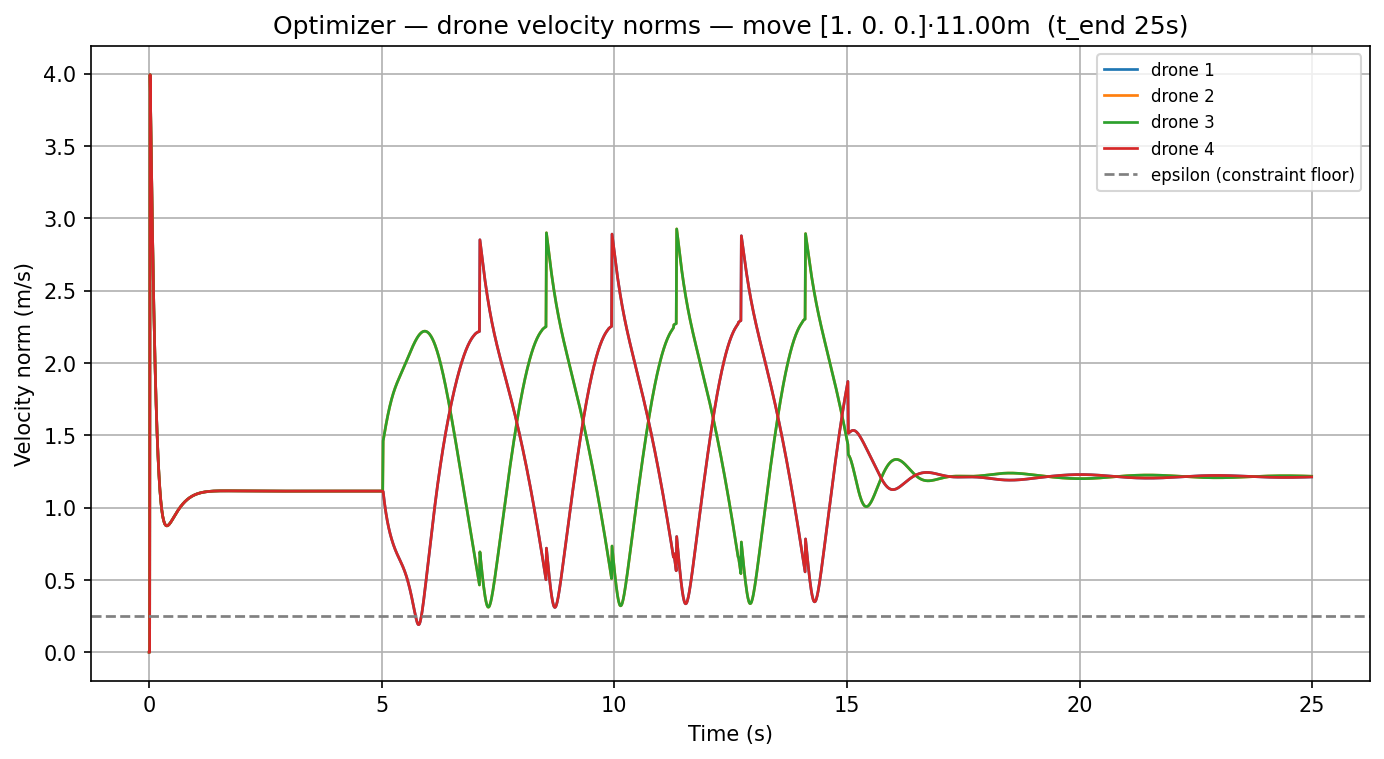
\includegraphics[width=0.8\textwidth]{figures/fig-expert-velocities.png}
  \caption{CCS carrier velocity norms for the same trajectory.}
  \label{fig:expert-velocities}
\end{figure}


\begin{figure}[H]
  \centering
  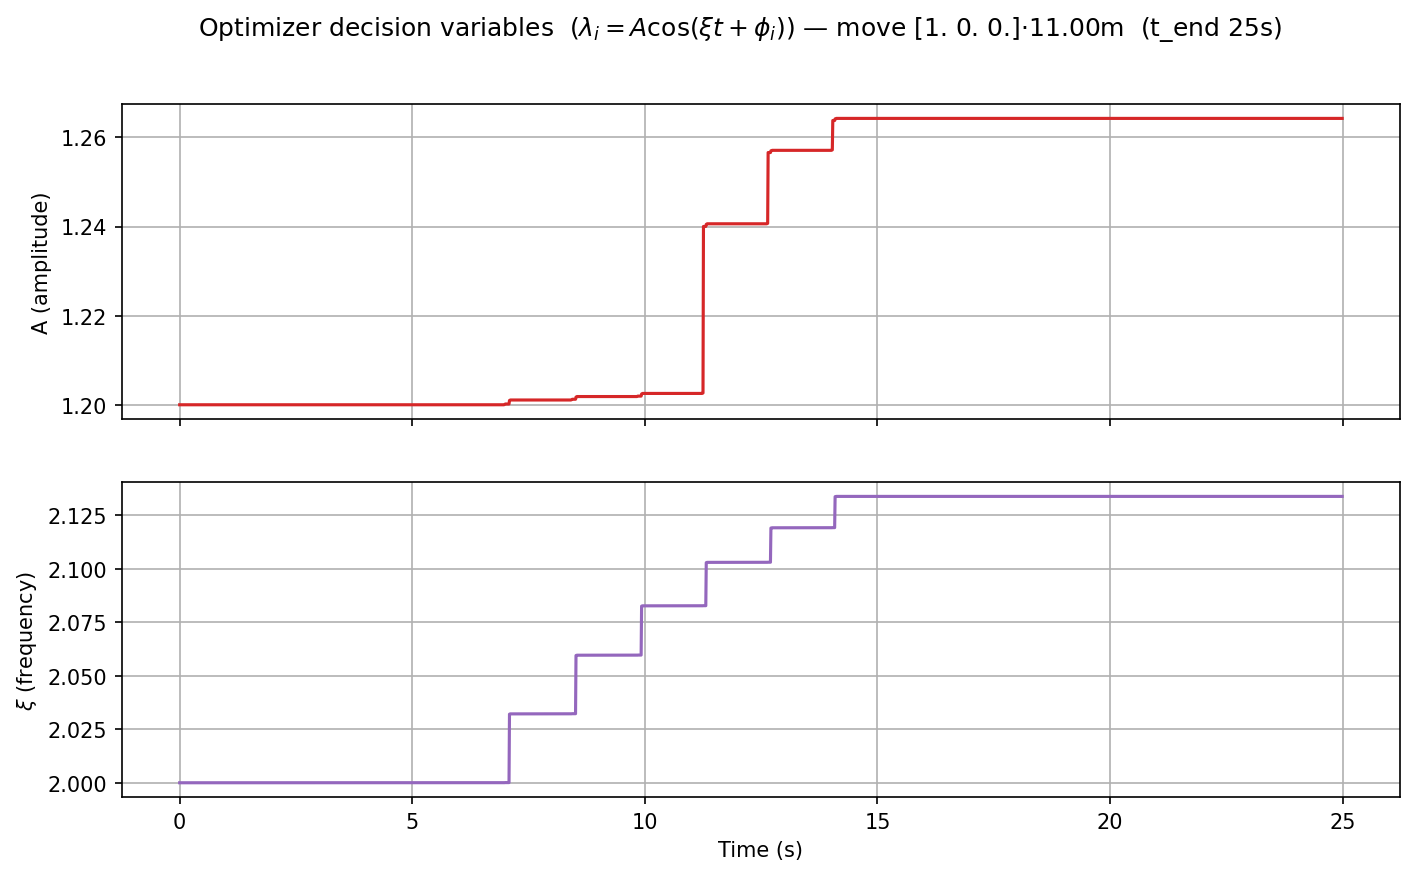
\includegraphics[width=0.8\textwidth]{figures/fig-expert-decision-vars.png}
  \caption{Optimizer decision variables $\lambda_i = A\cos(\xi t + \phi_i)$ for the same trajectory.}
  \label{fig:expert-decision-vars}
\end{figure}

We see in the two figures abotve that as soon as the minimum velocity is 
violated the optimizer reacts and changes $A$ and $\xi$ and accordingly the 
velocity norms change and do not dip below epsilon again. 

\newpage
\subsubsection{Supervised Learning}

Initially, the policy was trained with supervised learning only. In this 
section, we show how it performs and why it was not enough.

\begin{figure}[H]
  \centering
  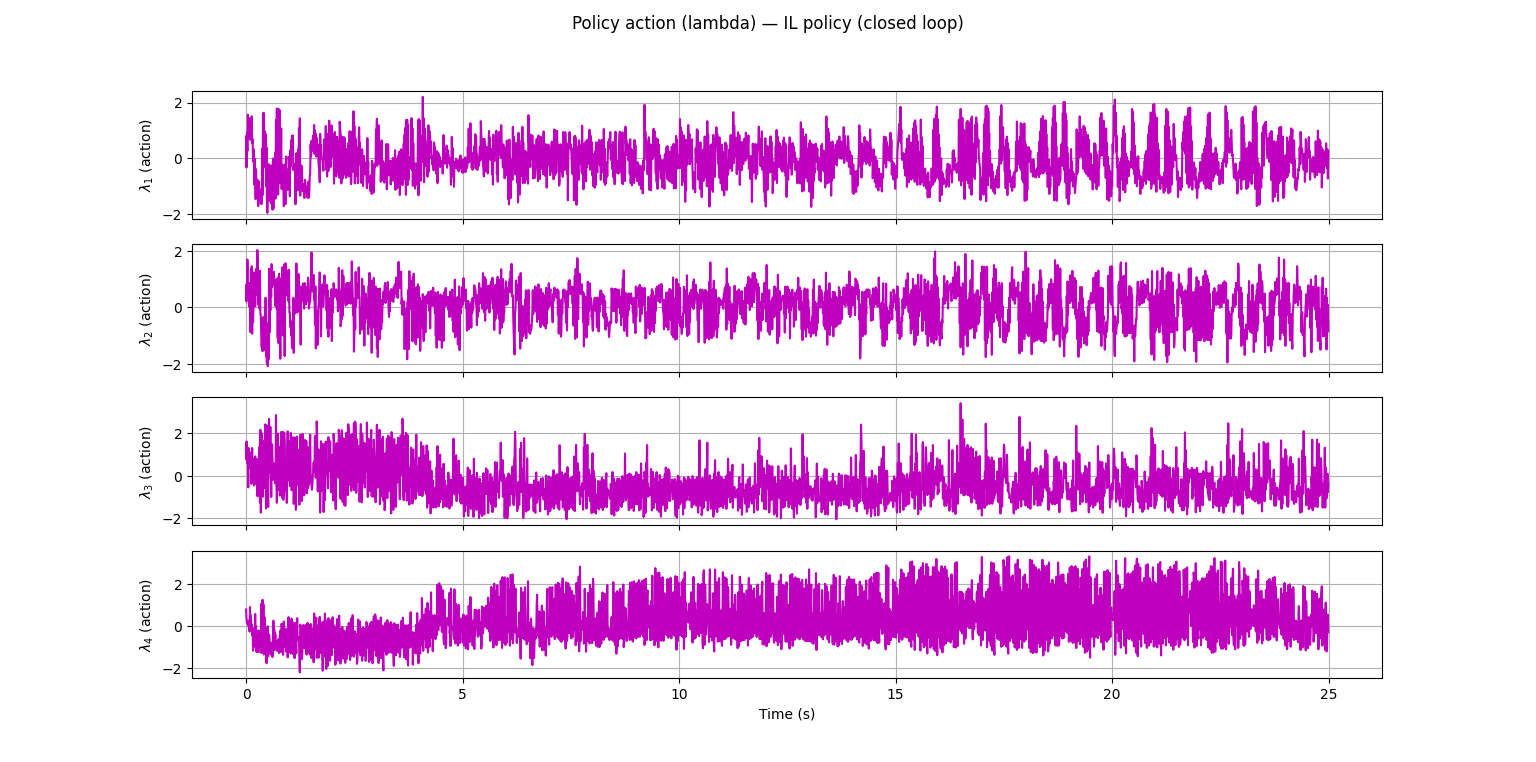
\includegraphics[width=\textwidth,height=10cm]{figures/fig-sl-lambda.png}
  \caption{$\lambda$ produced by the supervised-only policy while flying, showing uncontrolled jitter.}
  \label{fig:sl-lambda}
\end{figure}

Even though the MSE after the supervised learning was $< 1\times10^{-3}$,
deploying the policy in closed loop is much more unstable and leads to huge
jittering in $\lambda$ due to the distribution shift discussed in Section~\ref{sec:dagger}. 
For this reason,
using supervised learning alone is not enough and DAgger becomes necessary.


\begin{figure}[H]
  \centering
  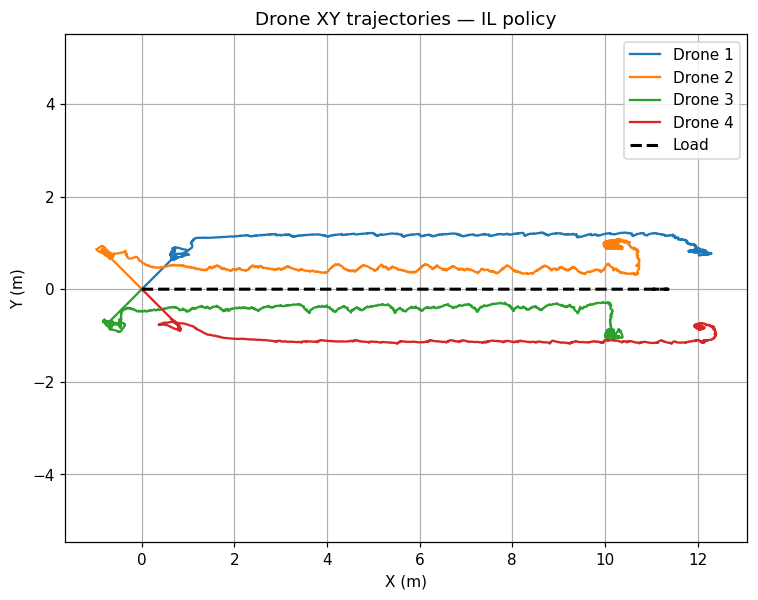
\includegraphics[width=0.8\textwidth]{figures/fig-sl-xy-trajectories.png}
  \caption{Carriers and load Trajectory top view (X-Y) trajectories of the policy trained with supervised learning only.}
  \label{fig:sl-xy-trajectories}
\end{figure}

We notice that the load trajectory is not changed (still following the 
reference) even though the $\lambda$'s are completely corrupted. This is due to
the strict separation of the internal forces (that operate in the nullspace
of the grasp matrix) and the forces affecting the load. The internal forces
only affect the carrier trajectory partially, however, it is enough to make it 
physically unfeasible. These results must be interpreted with care, as the 
simulation might indicate that the load tracking is working or that the 
carriers are following a jittery trajectory, while if we run this in real life
it will probably fail due to the high jitter.

\begin{figure}[H]
  \centering
  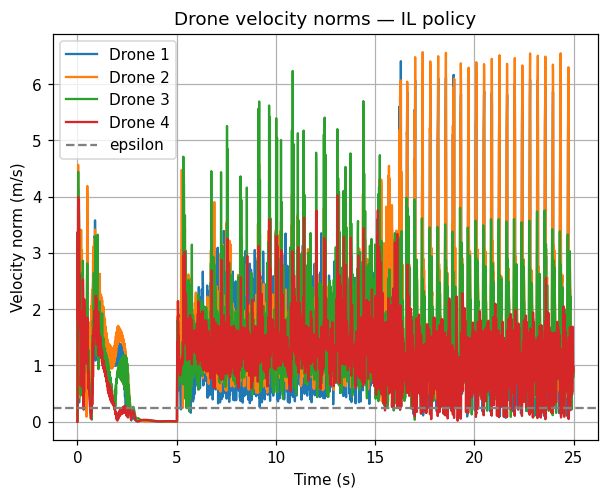
\includegraphics[width=0.8\textwidth]{figures/fig-sl-velocity-norms.png}
  \caption{Drone velocity norms of the policy trained with supervised learning only.}
  \label{fig:sl-velocity-norms}
\end{figure}

This plot again highlights the same idea mentioned before. The load tracking
its reference trajectory in the simulation does not mean that it will actually
do in real life. This plot shows that the carriers' velocities are very
jittery and dip many times below epsilon and even reach zero for a considerable
period of time. Therefore we can firmly conclude that the policy is failing.
A plant model that captures these interactions can better reflect what will 
happen in real life but would be much more complicated to build and is outside
the scope of this work. Until this more accurate plant model is used, all
resulting plots must be evaluated with care to determine if the policy is 
successful of no. 

\subsubsection{DAgger}

The following figures compare the DAgger-trained policy (network) against the
optimizer (CCS) on the single reference trajectory.

\begin{figure}[H]
  \centering
  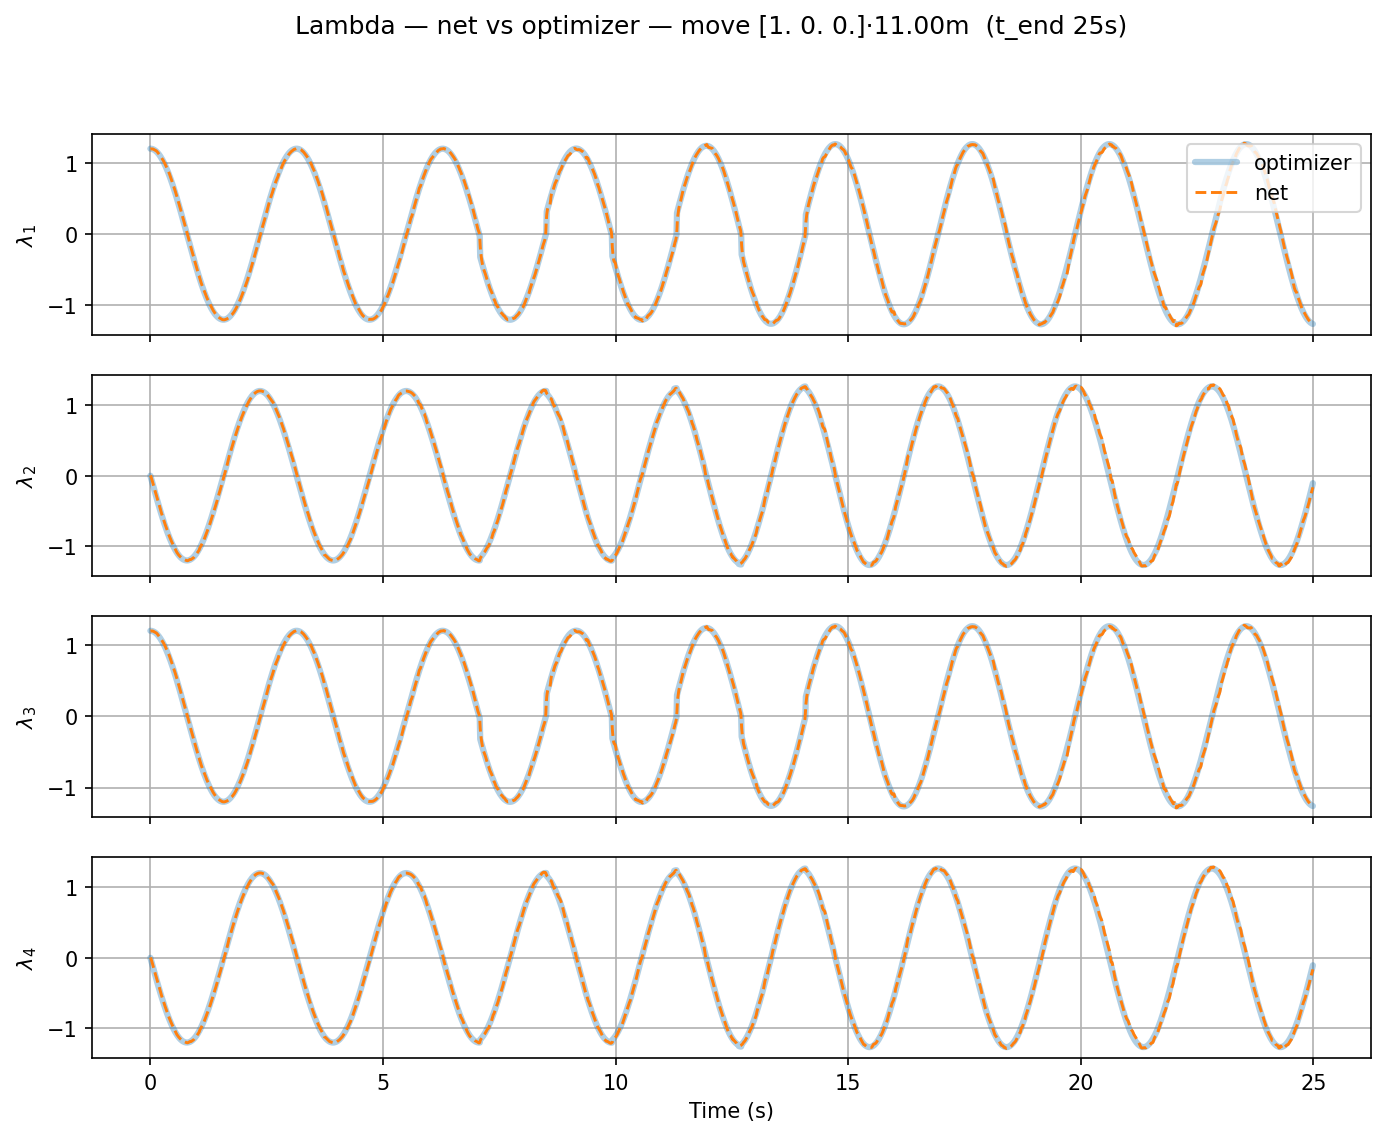
\includegraphics[width=0.8\textwidth]{figures/fig-f1-1trj-lambdas.png}
  \caption{$\lambda$ per carrier: DAgger-trained policy (network) vs optimizer.}
  \label{fig:f1-1trj-lambdas}
\end{figure}

As it can be seen in this plot, the DAgger-trained policy produces 
near-identical output to the optimizer. This is the main output and 
everything else is downstream from it. Therefore, we expect the other plots to
show satisfactory performance. Refer to table 5.1 for a numerical comparison. 

\begin{figure}[H]
  \centering
  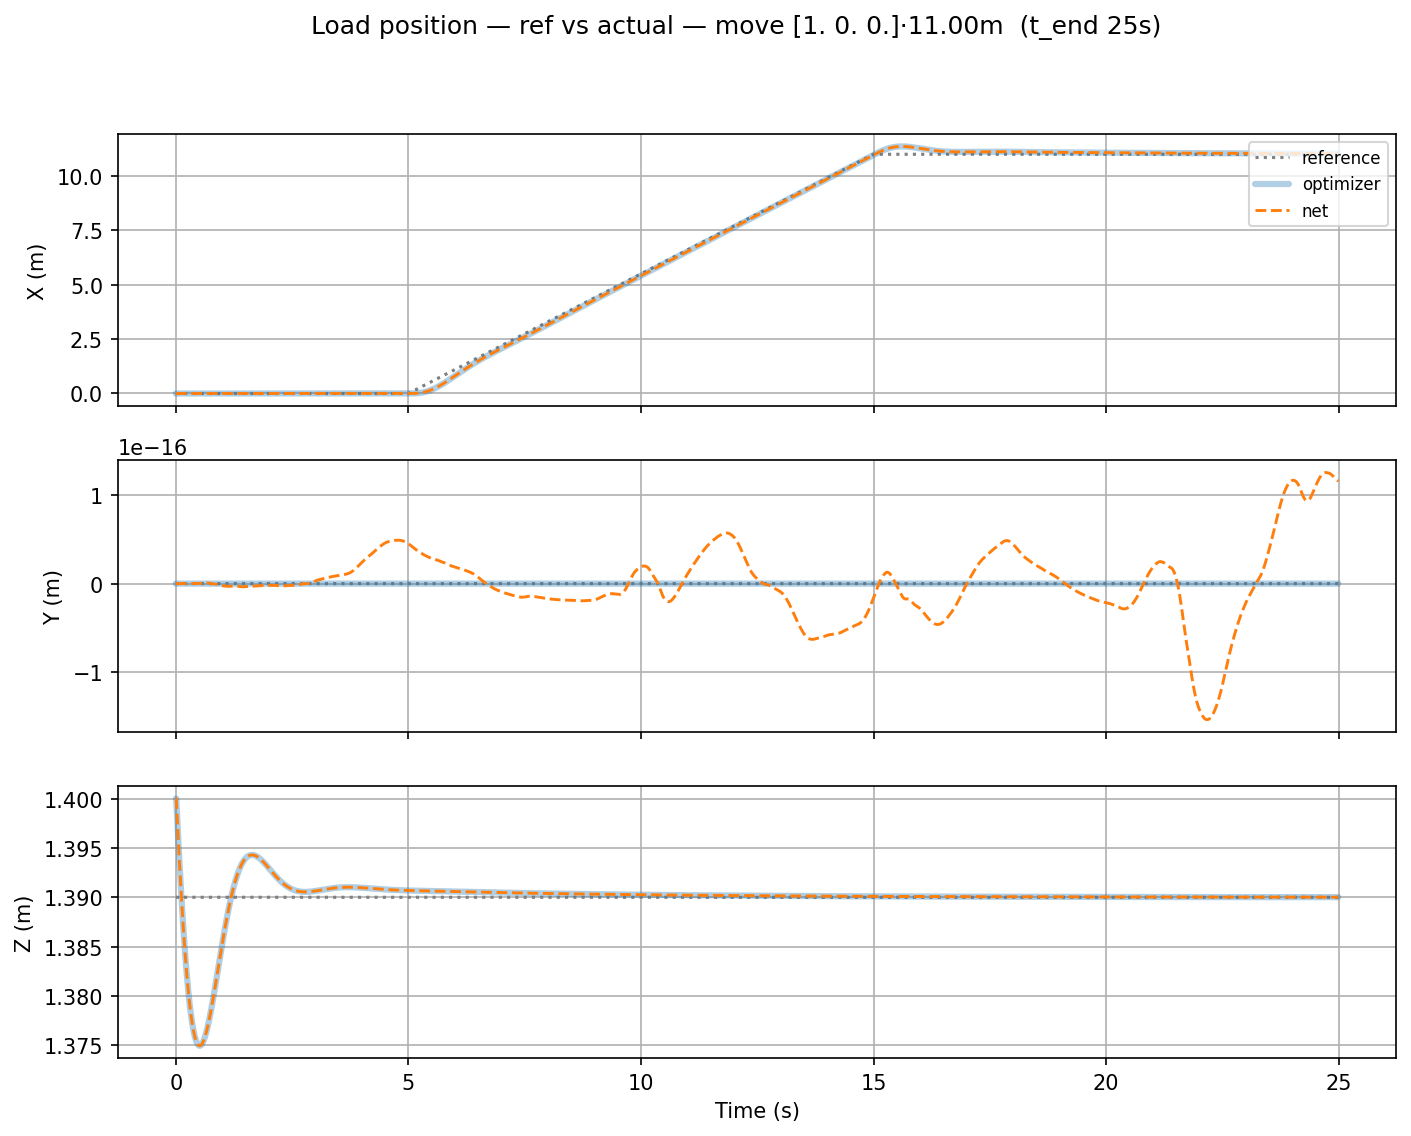
\includegraphics[width=0.8\textwidth]{figures/fig-f1-1trj-load-tracking.png}
  \caption{Load position tracking ($X/Y/Z$): reference vs network and optimizer.}
  \label{fig:f1-1trj-load-tracking}
\end{figure}

\begin{figure}[H]
  \centering
  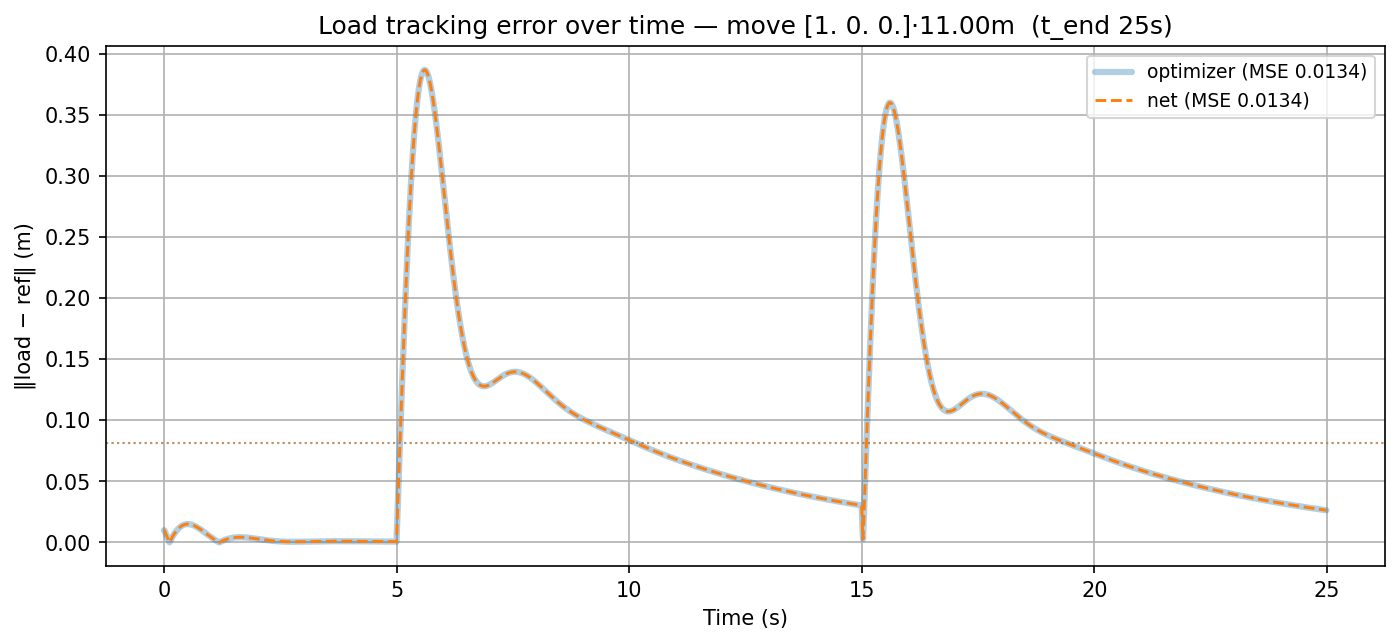
\includegraphics[width=0.8\textwidth]{figures/fig-f1-1trj-load-error.png}
  \caption{Load tracking error $\lVert\text{load}-\text{ref}\rVert$ over time: network vs optimizer.}
  \label{fig:f1-1trj-load-error}
\end{figure}

The last two plots show that the load tracking is not changed by swapping the
optimizer with the net(note that the scale on the Y-axis is 1e-16). This is 
expected as by design they do not affect the load tracking forces/wrench. 

\begin{figure}[H]
  \centering
  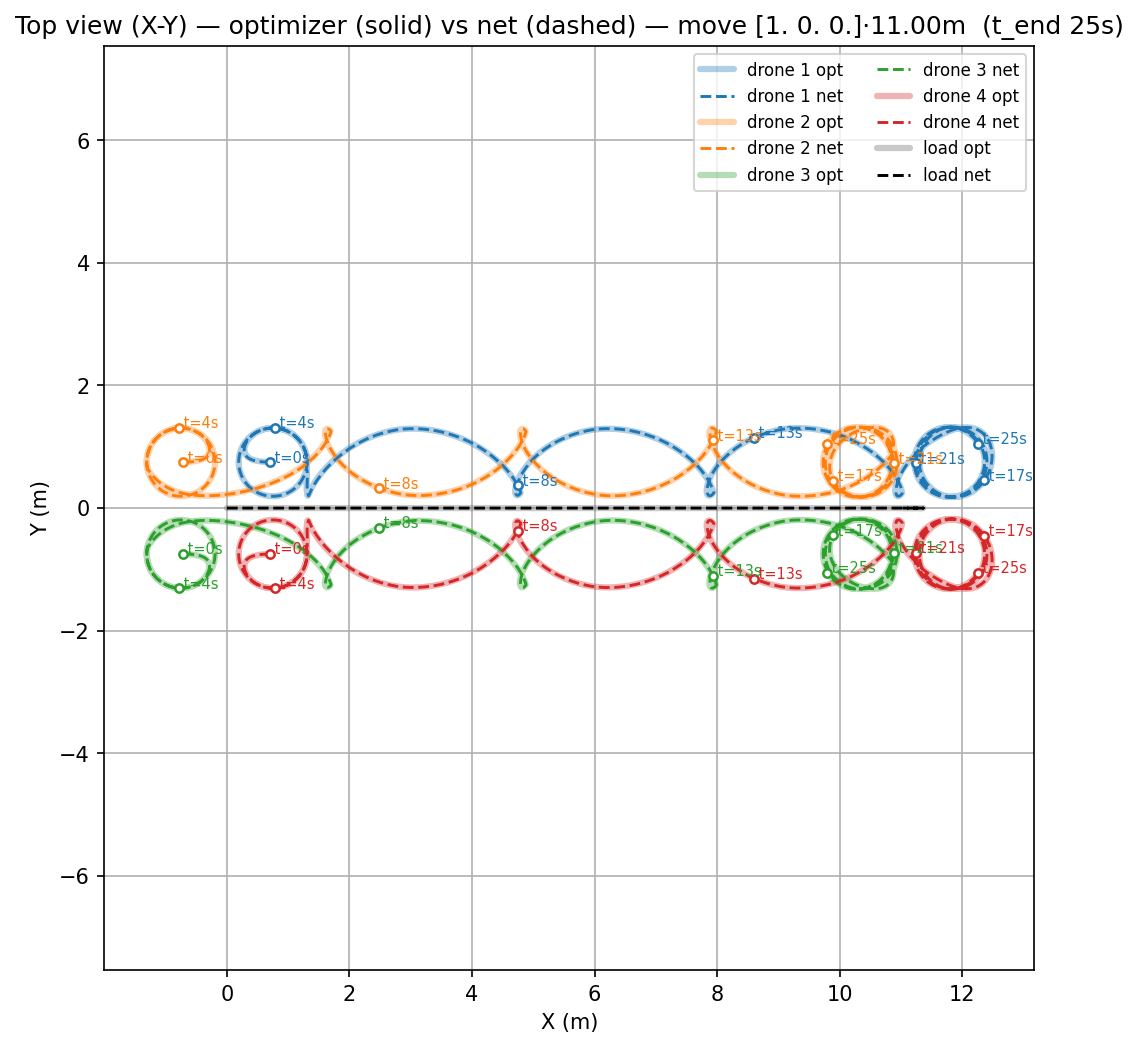
\includegraphics[width=0.9\textwidth]{figures/fig-f1-1trj-topview.png}
  \caption{Carrier and load trajectories, top view ($X$-$Y$): network vs optimizer.}
  \label{fig:f1-1trj-topview}
\end{figure}

\begin{figure}[H]
  \centering
  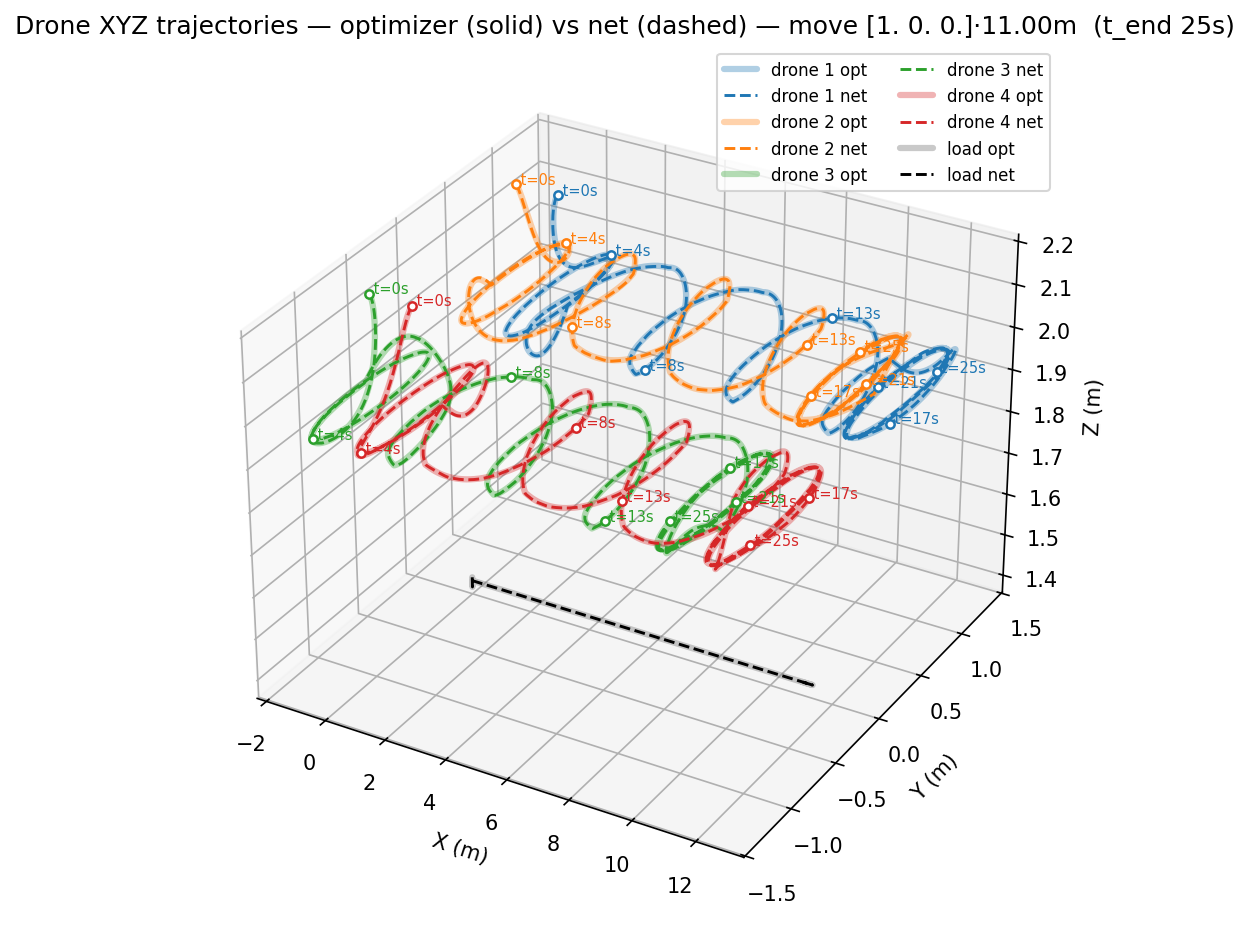
\includegraphics[width=0.7\textwidth]{figures/fig-f1-1trj-xyz.png}
  \caption{Carrier and load trajectories ($X$-$Y$-$Z$): network vs optimizer.}
  \label{fig:f1-1trj-xyz}
\end{figure}

We can see that the carrier trajectories produced by the net overlap with
the trajectories produced by the CCS with the optimizer. This is expected
since the $\lambda$'s are overlapping.  

\begin{figure}[H]
  \centering
  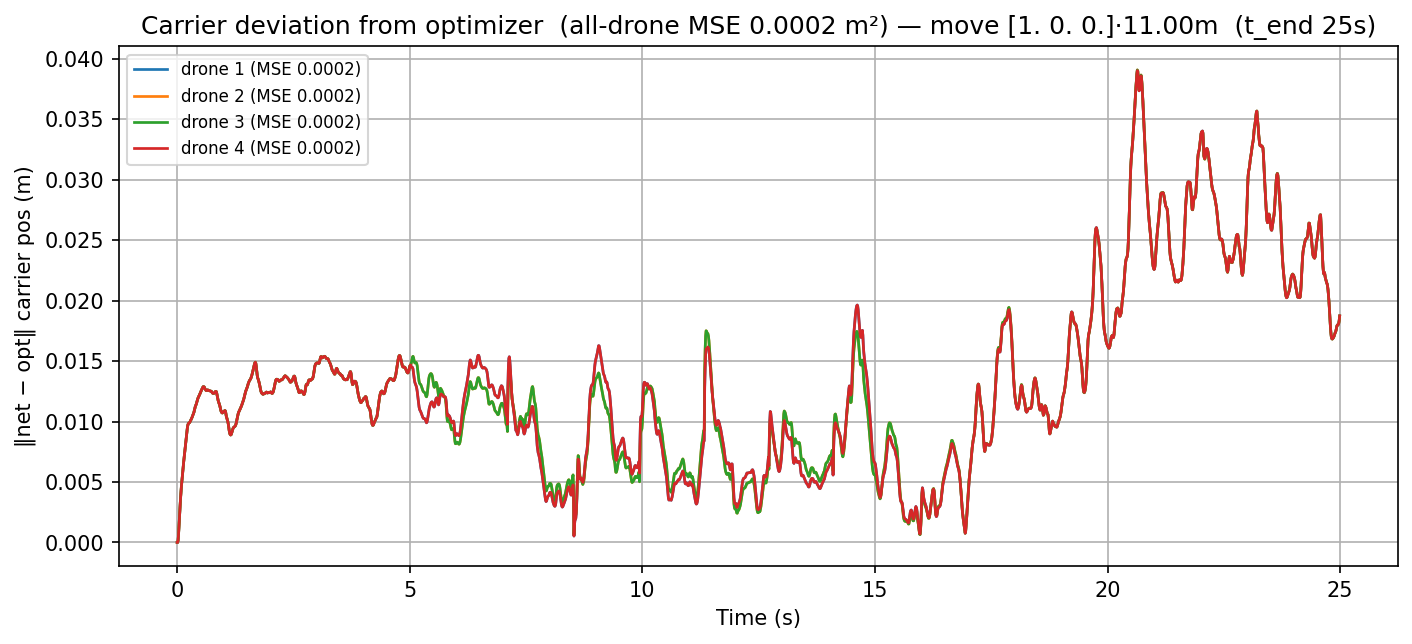
\includegraphics[width=0.8\textwidth]{figures/fig-f1-1trj-carrier-dev.png}
  \caption{Per-carrier position deviation of the network from the optimizer over time.}
  \label{fig:f1-1trj-carrier-dev}
\end{figure}

We can see that the deviation in general is low and remains bounded below 
0.04m (4cm) throughout the episode. While the error trends up from around
t = 15s to t = 20s, it stabilizes and even trends down from t = 20s to 
t = 25s. We hypothesize that this behavior is due to the delayed
effect of the historical $\lambda$'s in the network input. In other words,
when $A$ and $\xi$ change mid-trajectory, it takes some time until the 
historical $\lambda$'s in the observation space are all produced by these new 
values. Therefore, when $A$ and $\xi$ change quickly, the deviation rises but
then over time it stabilizes and goes back down after the net adjusts itself
to the new values.

\begin{figure}[H]
  \centering
  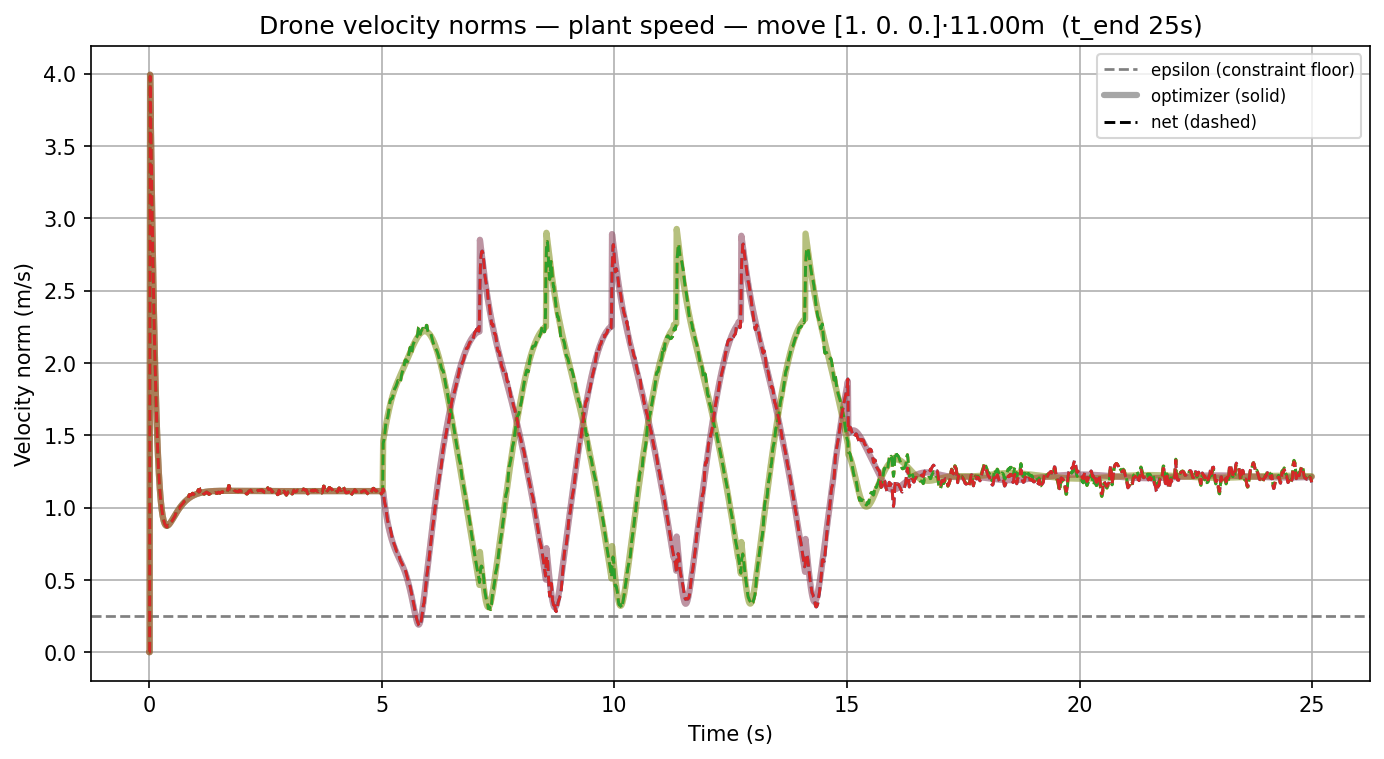
\includegraphics[width=0.8\textwidth]{figures/fig-f1-1trj-vnorms.png}
  \caption{Carrier velocity norms: network vs optimizer, with the $\epsilon$ constraint floor.}
  \label{fig:f1-1trj-vnorms}
\end{figure}

We can see that the velocity norms overlap and that the net has learnt to 
respond to the minimum velocity violation in the exact same way as the 
optimizer. While it is a bit noiser especially towards the latter part
of the episode, the noise is generally very small in magnitude.

\begin{table}[H]
  \centering
  \caption{Performance of the DAgger-trained policy (network) on the single trajectory.}
  \label{tab:dagger-single-trajectory}
  \begin{tabular}{lcc}
    \hline
    \textbf{Metric} & \textbf{Network} & \textbf{Optimizer} \\
    \hline
    Load tracking MSE (m$^2$) & 0.01338 & 0.01338 \\
    Load tracking max error (m) & 0.38677 & 0.38677 \\
    \hline
    \multicolumn{3}{l}{\textbf{Carrier position deviation from optimizer, MSE (m$^2$)}} \\
    \hline
    Drone 1 & 0.00023 & -- \\
    Drone 2 & 0.00023 & -- \\
    Drone 3 & 0.00023 & -- \\
    Drone 4 & 0.00023 & -- \\
    All drones & 0.00023 & -- \\
    \hline
    \multicolumn{3}{l}{\textbf{$\lambda$ deviation from optimizer, MSE}} \\
    \hline
    Drone 1 & 0.00068 & -- \\
    Drone 2 & 0.00076 & -- \\
    Drone 3 & 0.00068 & -- \\
    Drone 4 & 0.00076 & -- \\
    All drones & 0.00072 & -- \\
    \hline
  \end{tabular}
\end{table}

The load tracking is identical to the fifth decimal (and potentially beyond 
that but it serves no practical purpose). This is expected as explained 
earlier due to the structure and decomposition of the forces. The $\lambda$
deviations mainly show up in the carrier positions' deviations but even then
they remain minor.

We can see that we have succeeded in the task of overfitting one trajectory.
Therefore it is reasonable to assume we have a potentially good state/input
and network architecture. Thus, we can proceed with adding more trajectories 
and generalization.  

\subsection{Analysis of failure modes}

Before we show generalization results, we show some of the failures 
encountered before obtaining these results. They are important to show 
because they guided the design choices that were discussed in the 
Methodology chapter. 

We will focus on showing the $\lambda$'s since they are the direct ouput of the 
net and everything else is derived from it. In other words, if our policy is
imitating the optimizer's $\lambda$'s correctly then we expect everything to be
simular. Furthermore, if the $\lambda$'s are not identical, then the learning is
not working and we need to analyze why at the $\lambda$'s level. Analyzing the 
other variables does not tell us what is the root cause of the problem.

\begin{figure}[H]
  \centering
  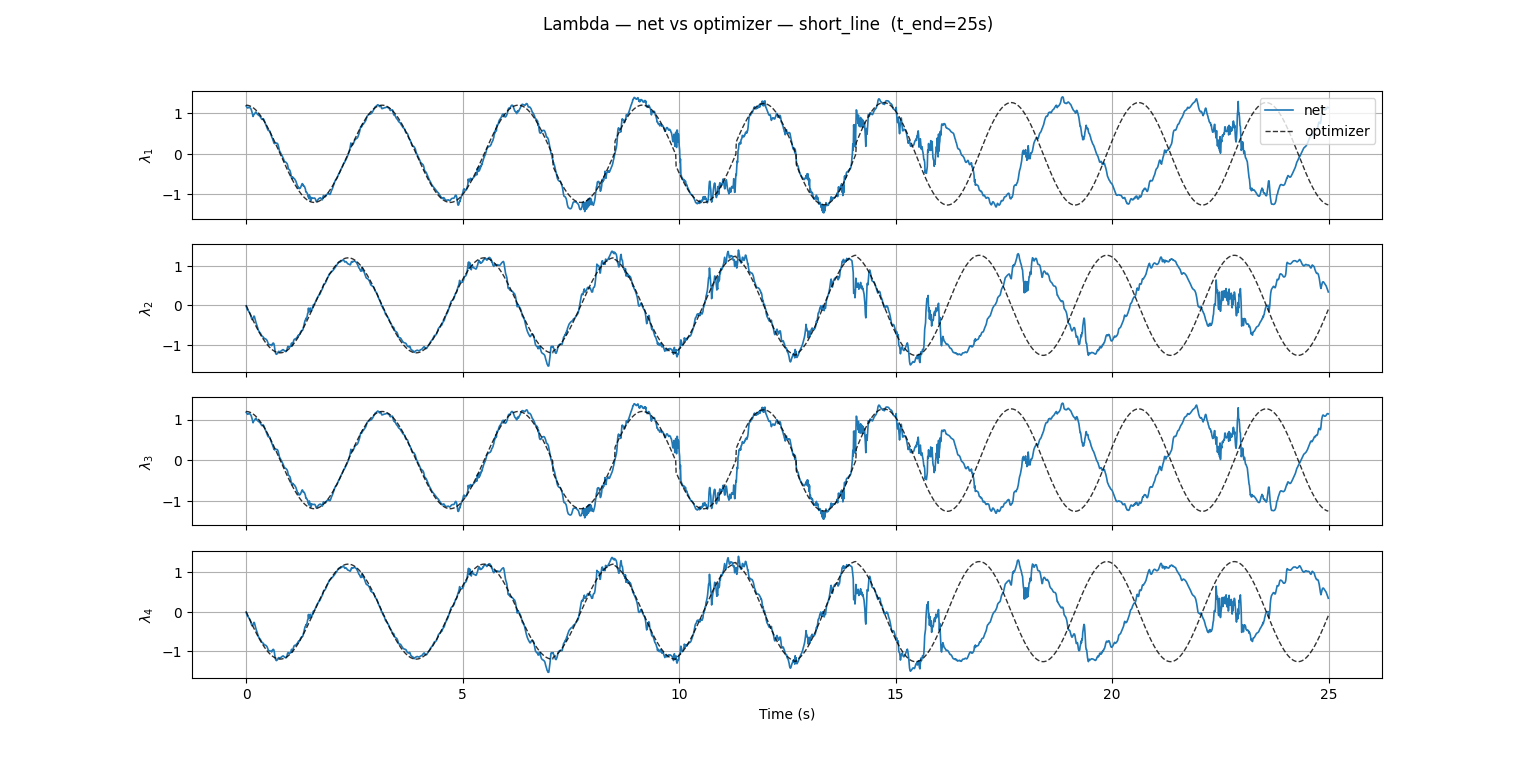
\includegraphics[width=\textwidth,height=10cm]{figures/fig-failure-short-line.png}
  \caption{$\lambda$'s produced by the network versus the optimizer on a short-line trajectory: the network tracks the optimizer closely at first, then diverges as errors compound.}
  \label{fig:failure-short-line}
\end{figure}

\begin{figure}[H]
  \centering
  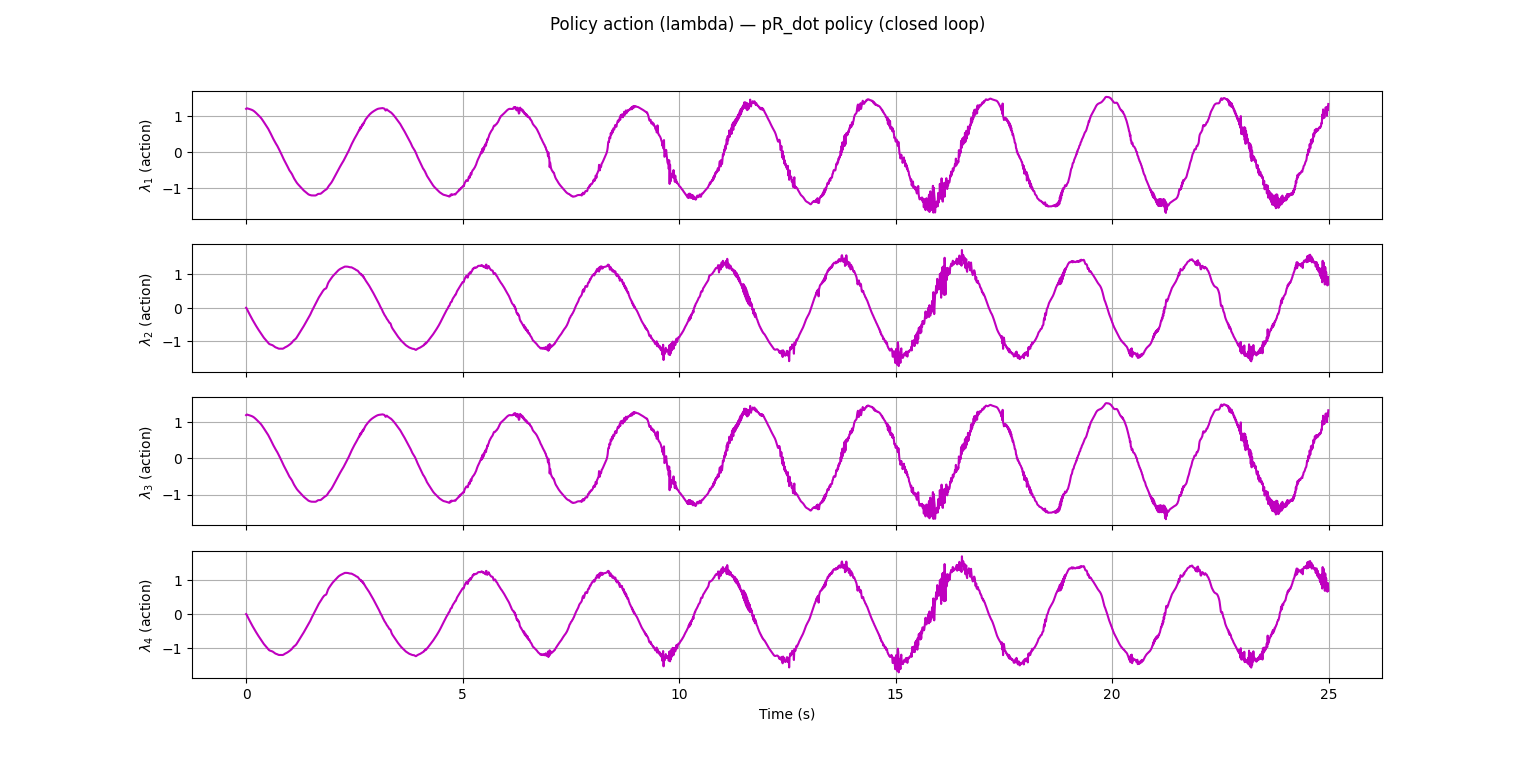
\includegraphics[width=\textwidth,height=10cm]{figures/fig-failure-prdot-policy.png}
  \caption{$\lambda$'s produced by a policy trained with $\dot p_R$ in the observation space, flown in closed loop: increasing high-frequency noise appears as the trajectory progresses.}
  \label{fig:failure-prdot-policy}
\end{figure}

\begin{figure}[H]
  \centering
  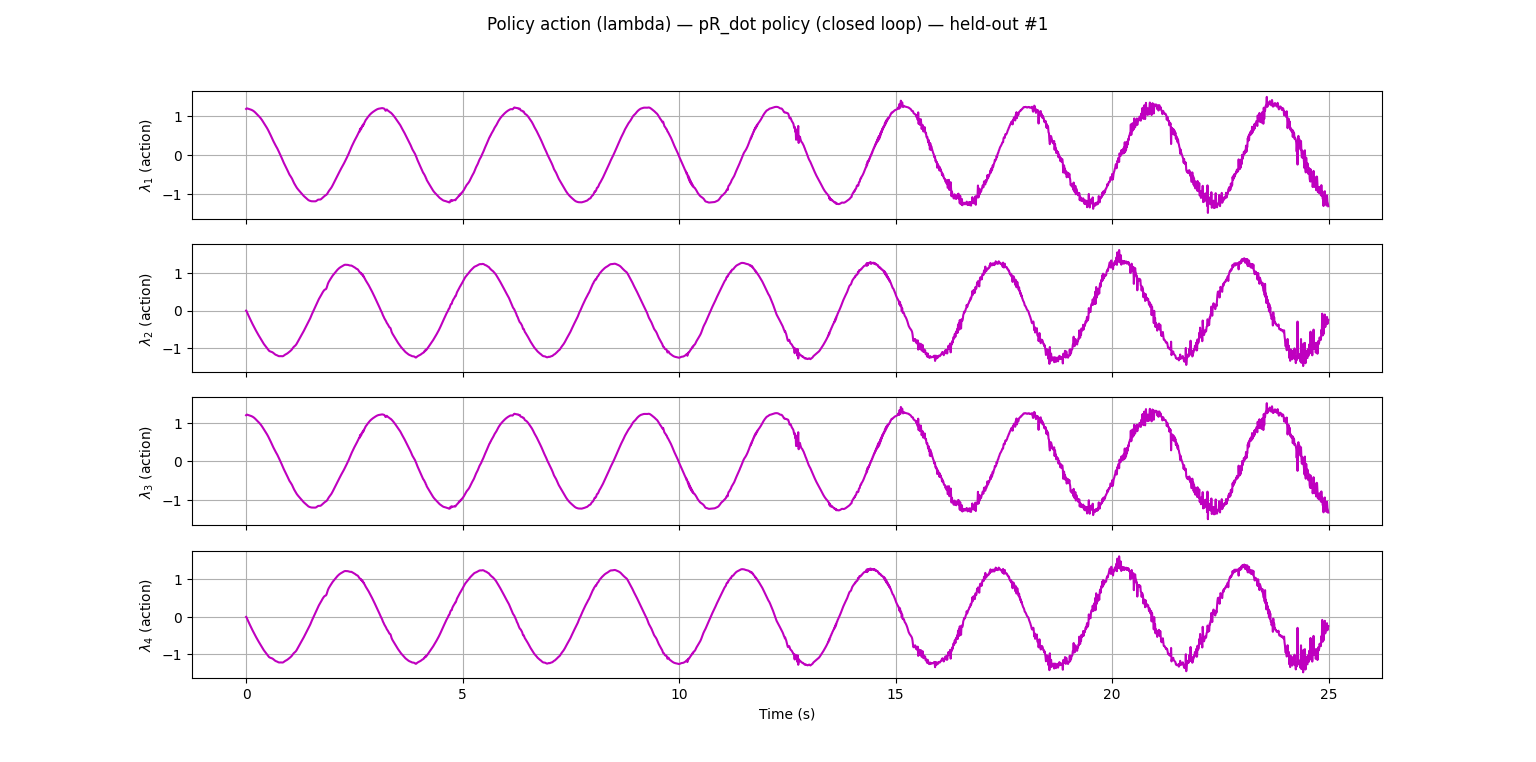
\includegraphics[width=\textwidth,height=10cm]{figures/fig-failure-prdot-heldout.png}
  \caption{$\lambda$'s produced by the same $\dot p_R$ policy on a held-out trajectory: the same noise issue appears, showing it is not specific to a single trajectory.}
  \label{fig:failure-prdot-heldout}
\end{figure}

\subsection{Generalization}

\subsubsection{Generalization across time}

\noindent\textbf{Longer-time trajectory (move $[-0.06, -0.88, -0.47]\cdot3$\,m, ramp, 50\,s)}

\begin{figure}[H]
  \centering
  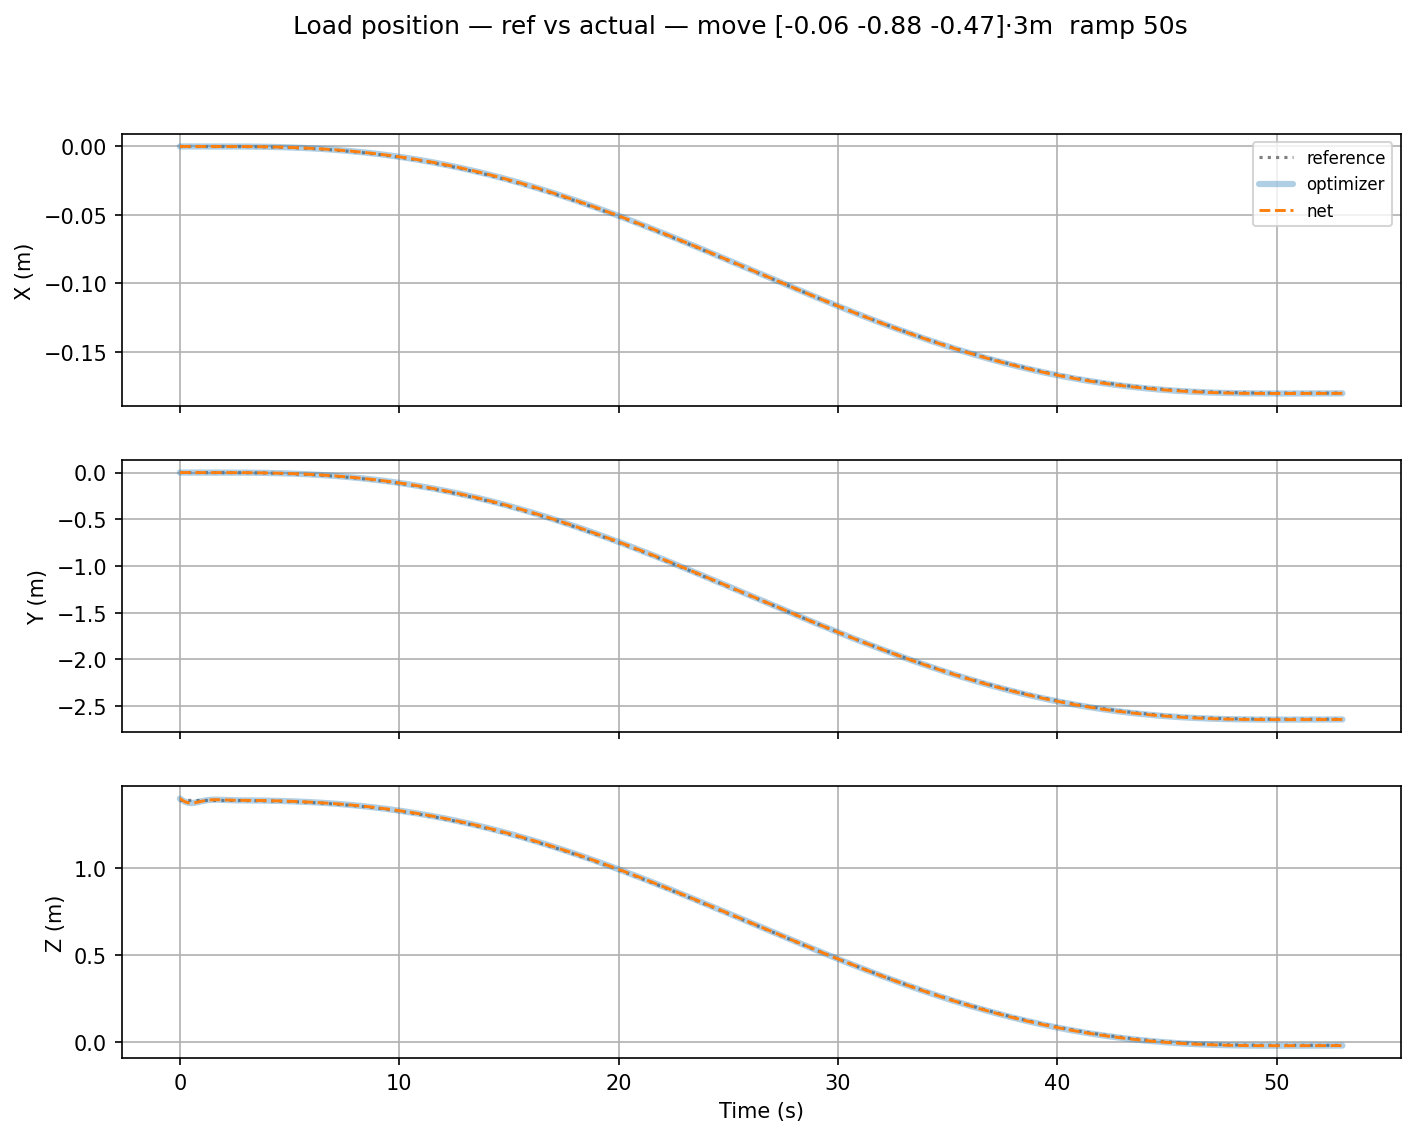
\includegraphics[width=0.8\textwidth]{figures/fig-gen-time-long-load-pos.png}
  \caption{Load position: reference vs.\ actual.}
  \label{fig:gen-time-long-load-pos}
\end{figure}

\begin{figure}[H]
  \centering
  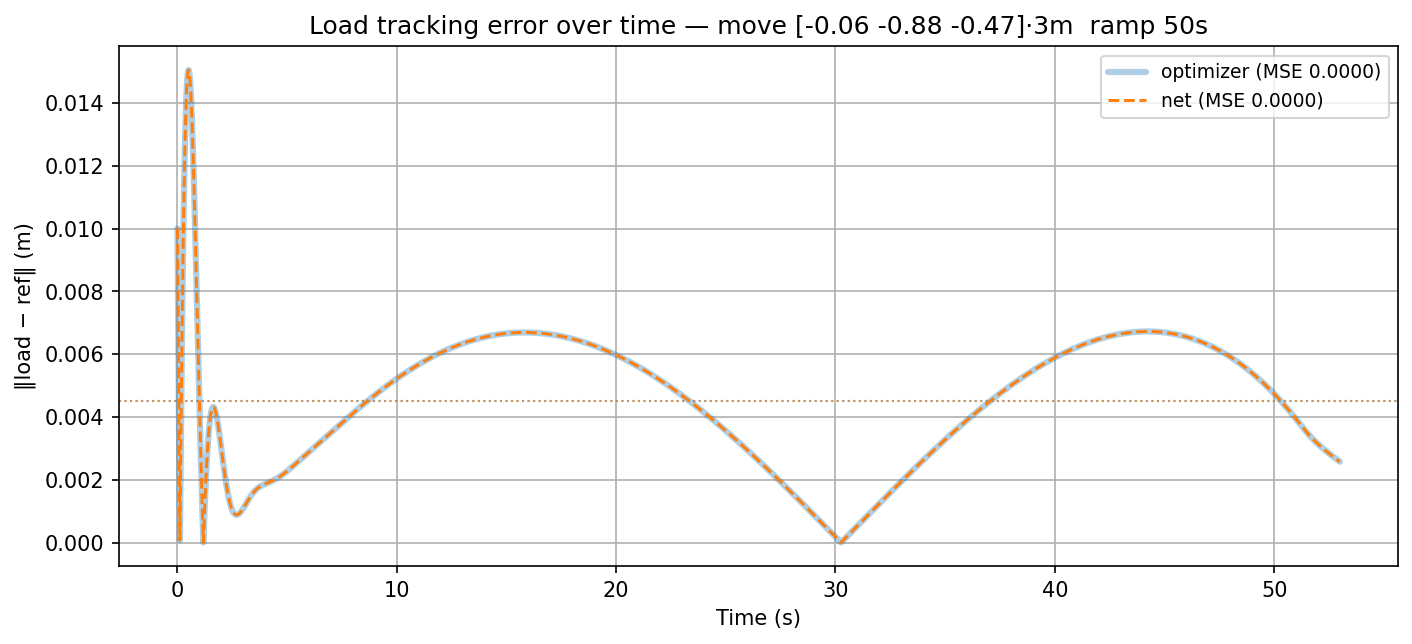
\includegraphics[width=0.8\textwidth]{figures/fig-gen-time-long-load-err.png}
  \caption{Load tracking error over time.}
  \label{fig:gen-time-long-load-err}
\end{figure}

\begin{figure}[H]
  \centering
  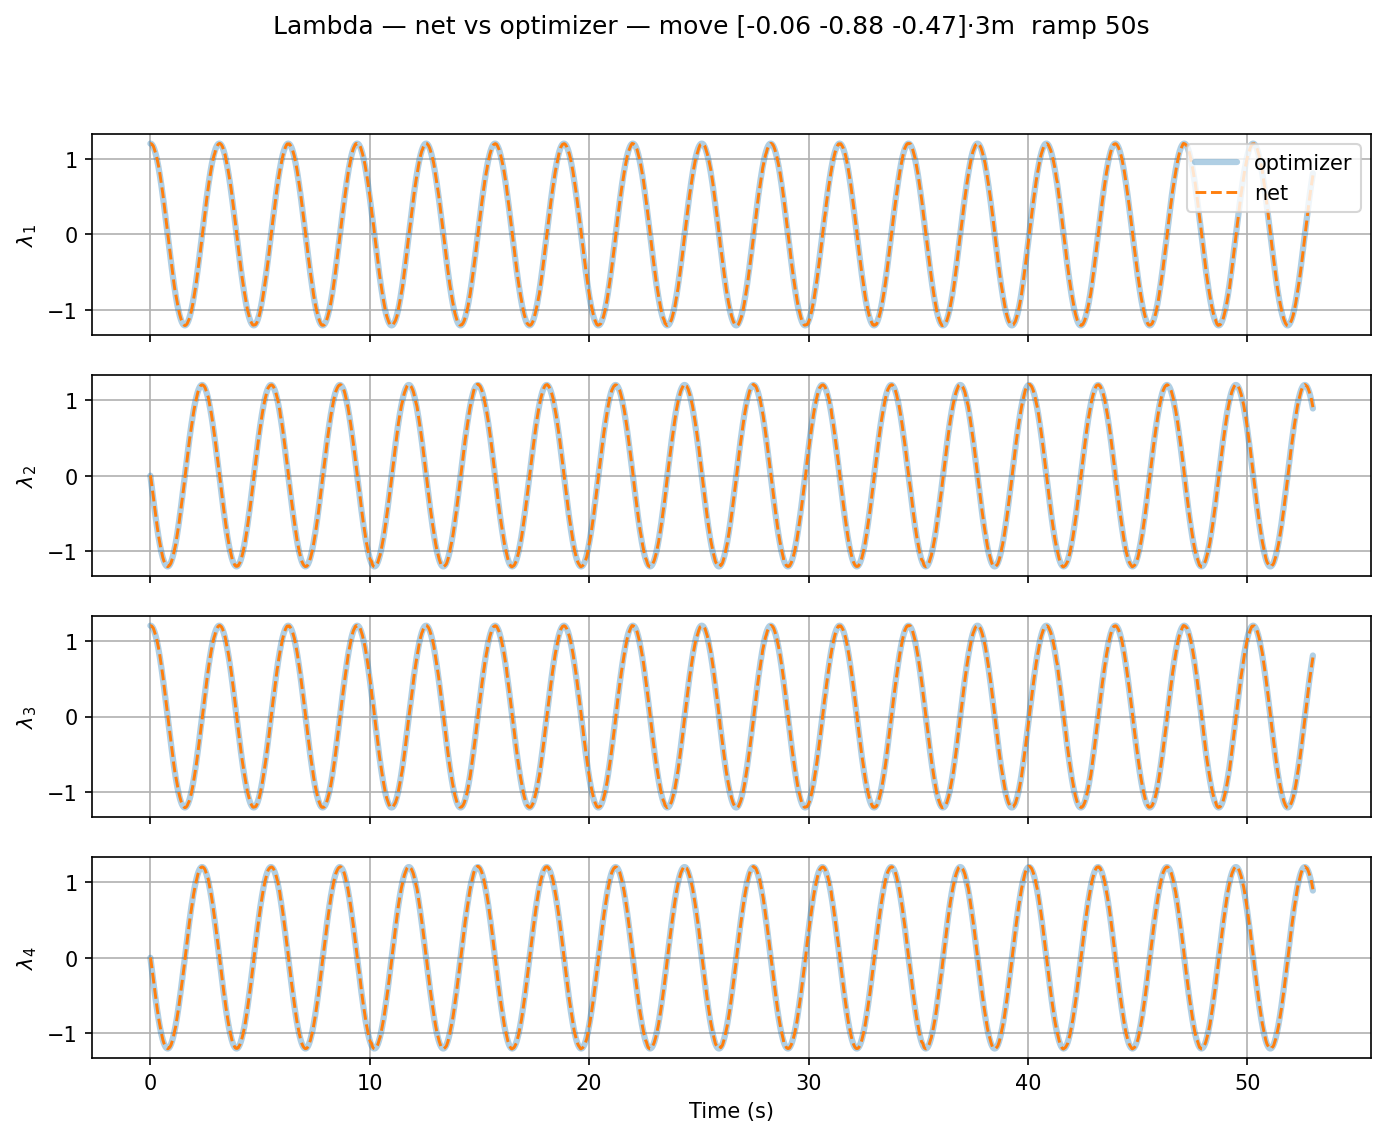
\includegraphics[width=0.8\textwidth]{figures/fig-gen-time-long-lambda.png}
  \caption{$\lambda$ produced by the network vs.\ the optimizer.}
  \label{fig:gen-time-long-lambda}
\end{figure}

\begin{figure}[H]
  \centering
  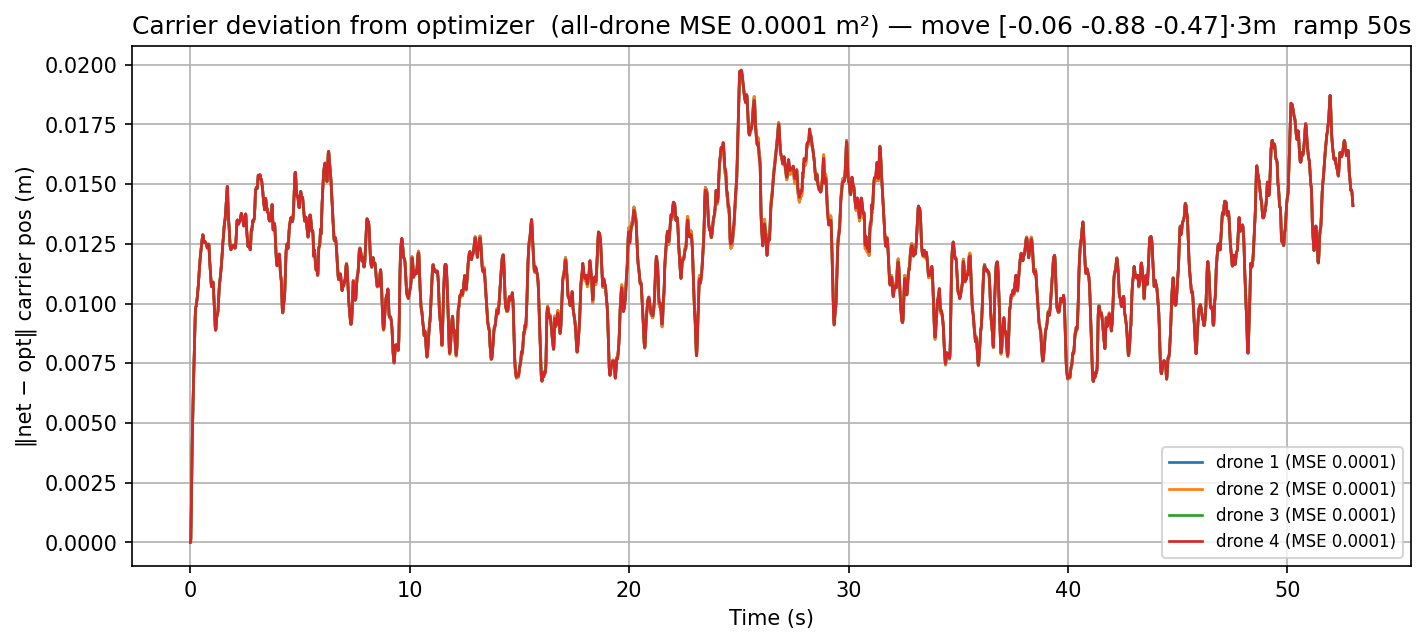
\includegraphics[width=0.8\textwidth]{figures/fig-gen-time-long-carrier-dev.png}
  \caption{Carrier deviation from the optimizer.}
  \label{fig:gen-time-long-carrier-dev}
\end{figure}

\begin{figure}[H]
  \centering
  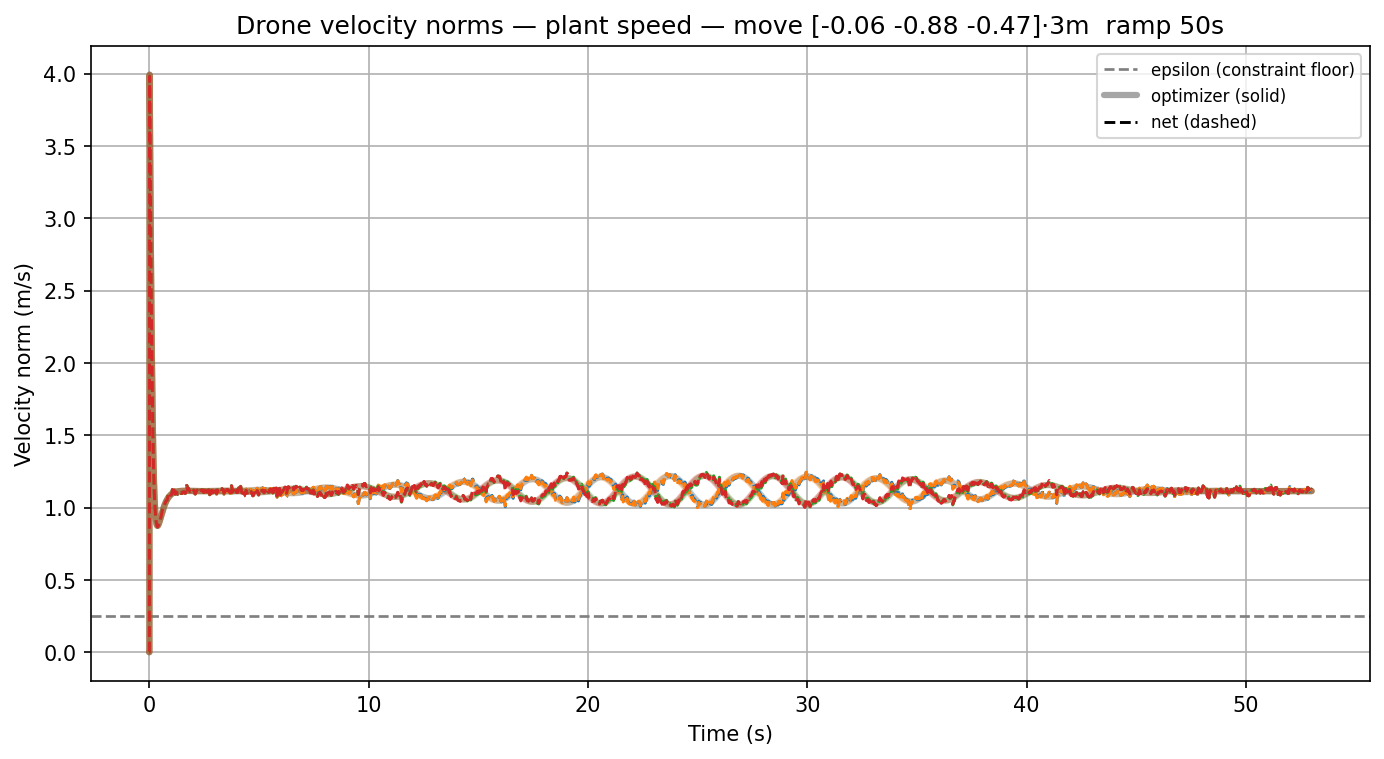
\includegraphics[width=0.8\textwidth]{figures/fig-gen-time-long-vnorms.png}
  \caption{Drone velocity norms (plant speed).}
  \label{fig:gen-time-long-vnorms}
\end{figure}

\begin{figure}[H]
  \centering
  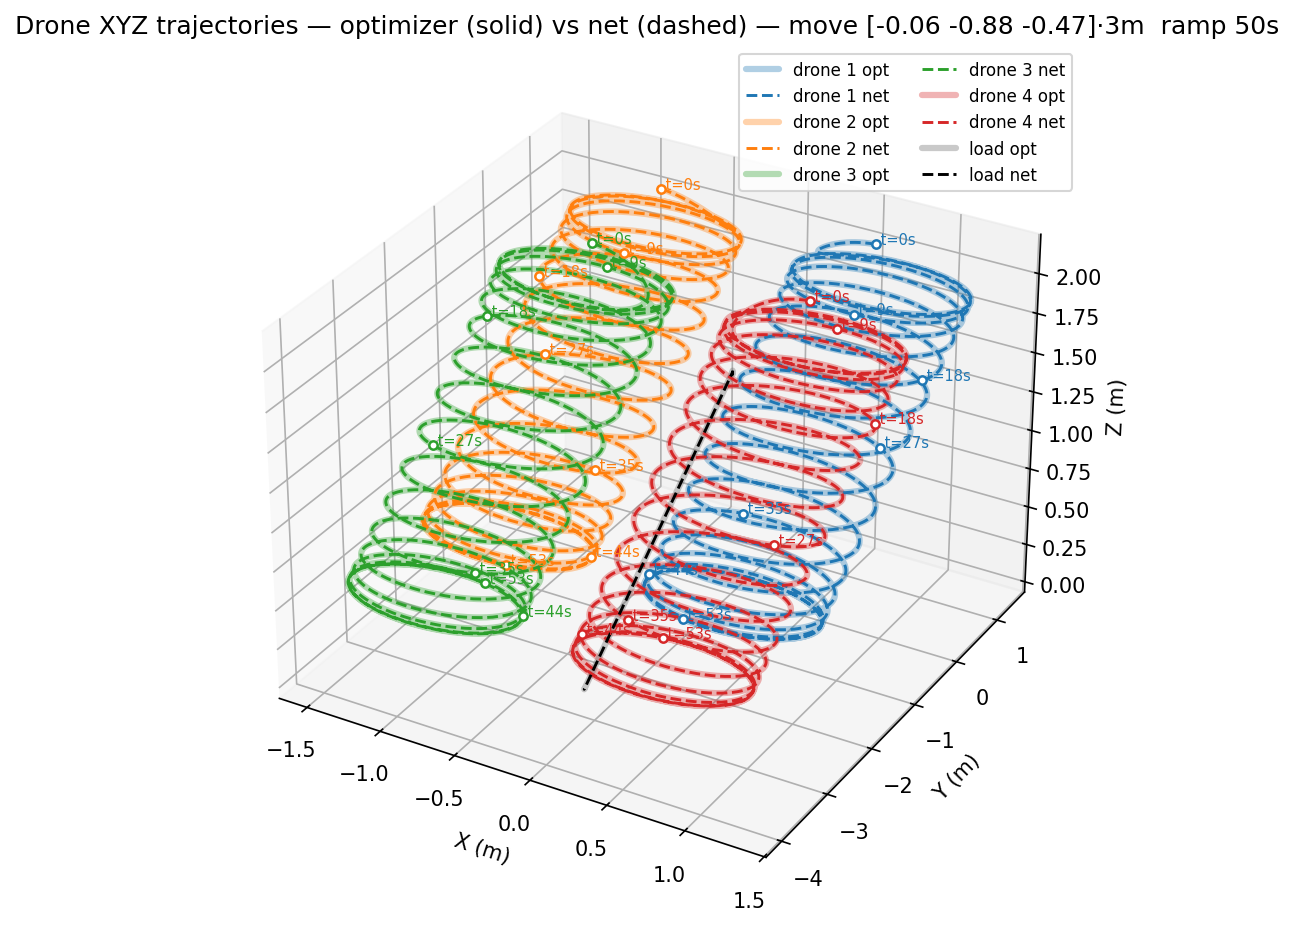
\includegraphics[width=0.8\textwidth]{figures/fig-gen-time-long-xyz.png}
  \caption{Drone XYZ trajectories: optimizer (solid) vs.\ net (dashed).}
  \label{fig:gen-time-long-xyz}
\end{figure}

\begin{table}[H]
  \centering
  \caption{Performance of the network on the longer-time generalization trajectory.}
  \label{tab:gen-time-long}
  \begin{tabular}{lcc}
    \hline
    \textbf{Metric} & \textbf{Network} & \textbf{Optimizer} \\
    \hline
    Load tracking MSE (m$^2$) & 0.00002 & 0.00002 \\
    Load tracking max error (m) & 0.01505 & 0.01505 \\
    \hline
    \multicolumn{3}{l}{\textbf{Carrier deviation from optimizer, MSE (m$^2$)}} \\
    \hline
    Drone 1 & 0.00015 & -- \\
    Drone 2 & 0.00015 & -- \\
    Drone 3 & 0.00015 & -- \\
    Drone 4 & 0.00015 & -- \\
    All drones & 0.00015 & -- \\
    \hline
    \multicolumn{3}{l}{\textbf{$\lambda$ deviation from optimizer, MSE}} \\
    \hline
    Drone 1 & 0.00035 & -- \\
    Drone 2 & 0.00038 & -- \\
    Drone 3 & 0.00035 & -- \\
    Drone 4 & 0.00038 & -- \\
    All drones & 0.00037 & -- \\
    \hline
  \end{tabular}
\end{table}

\noindent\textbf{Shorter-time trajectory (move $[-0.06, -0.88, -0.47]\cdot3$\,m, ramp, 20\,s)}

\begin{figure}[H]
  \centering
  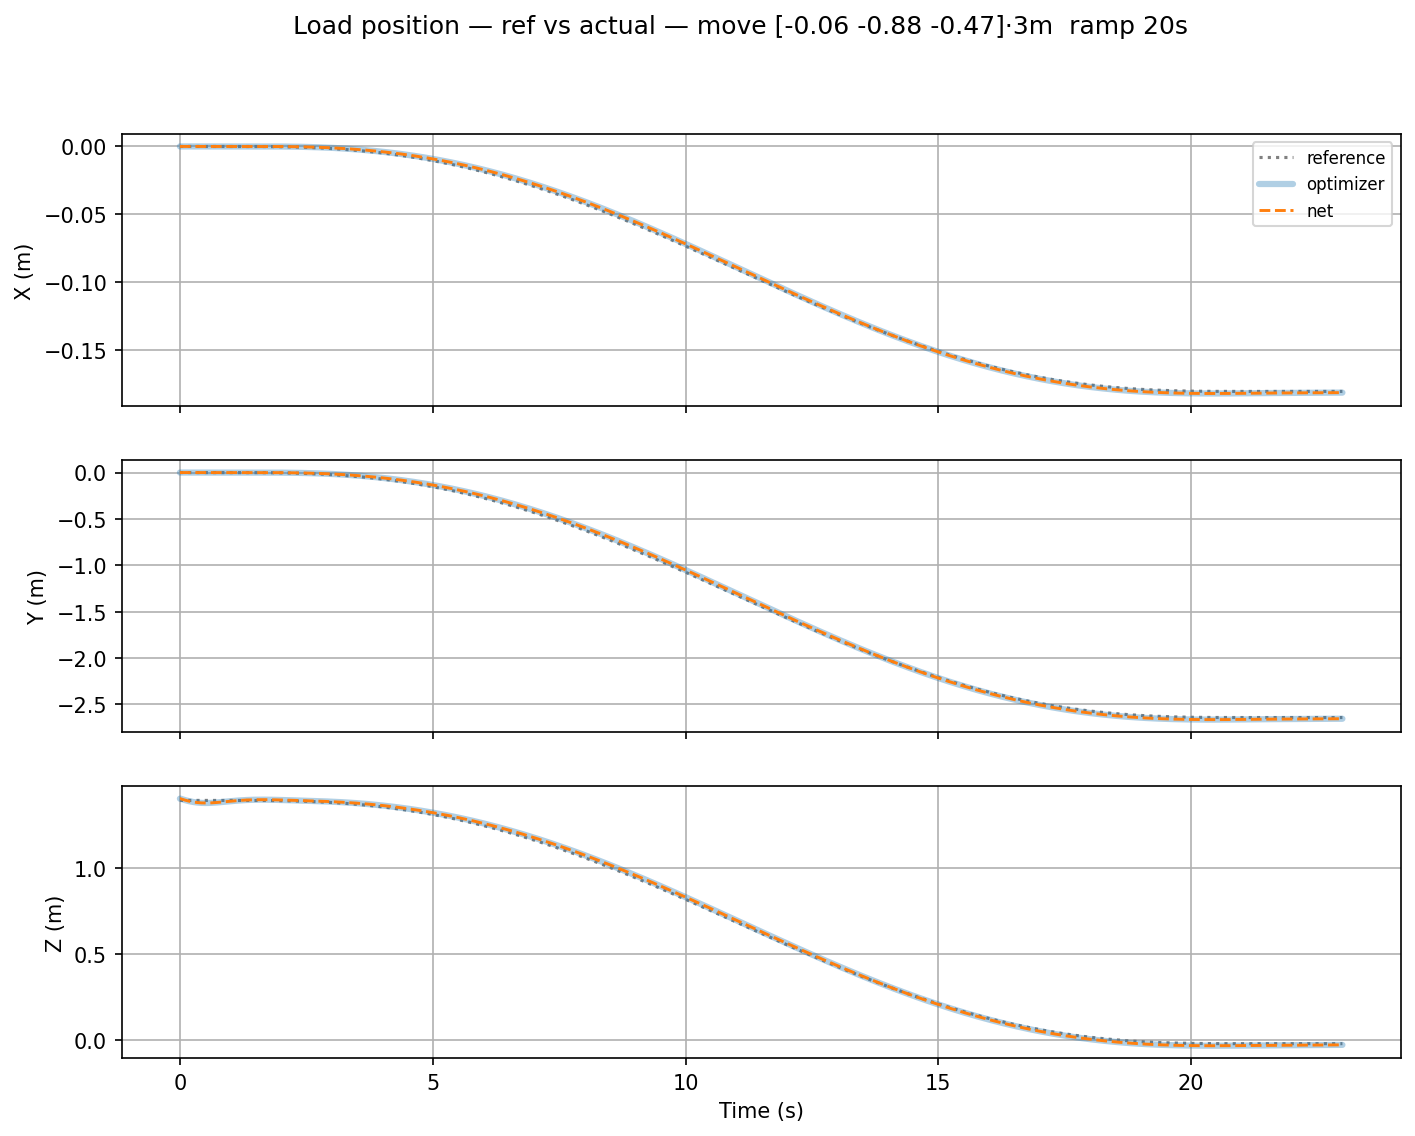
\includegraphics[width=0.8\textwidth]{figures/fig-gen-time-short-load-pos.png}
  \caption{Load position: reference vs.\ actual.}
  \label{fig:gen-time-short-load-pos}
\end{figure}

\begin{figure}[H]
  \centering
  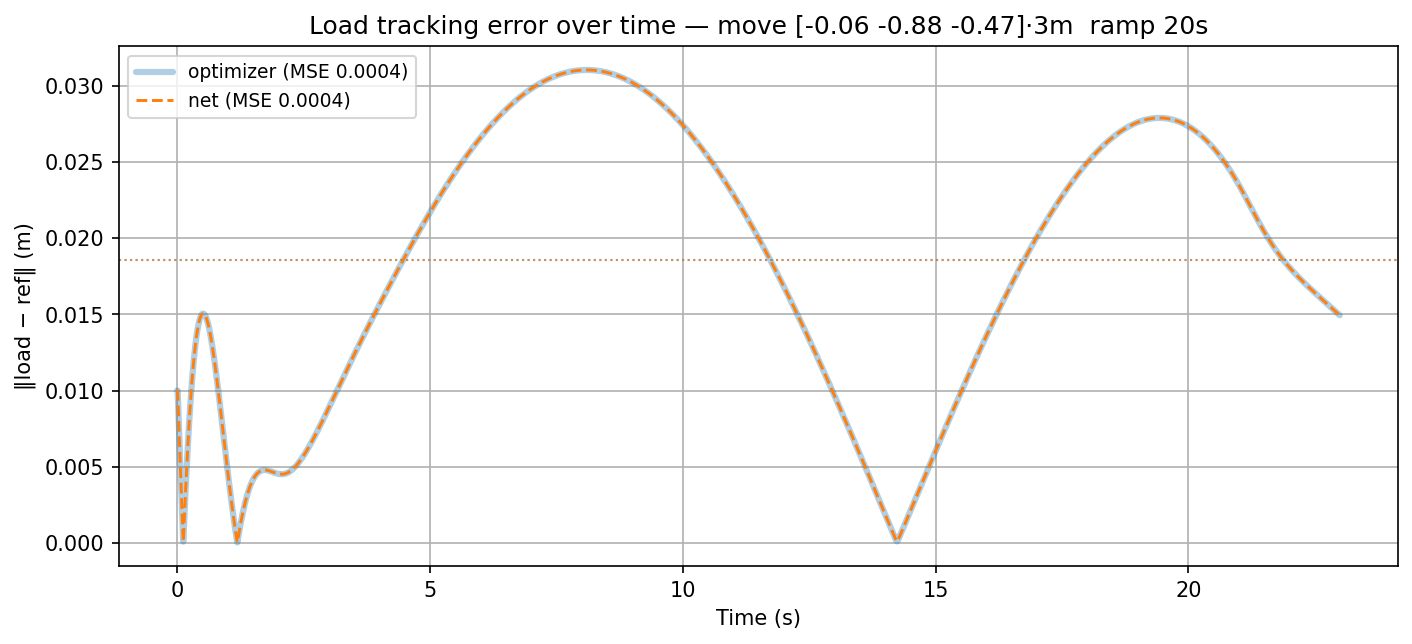
\includegraphics[width=0.8\textwidth]{figures/fig-gen-time-short-load-err.png}
  \caption{Load tracking error over time.}
  \label{fig:gen-time-short-load-err}
\end{figure}

\begin{figure}[H]
  \centering
  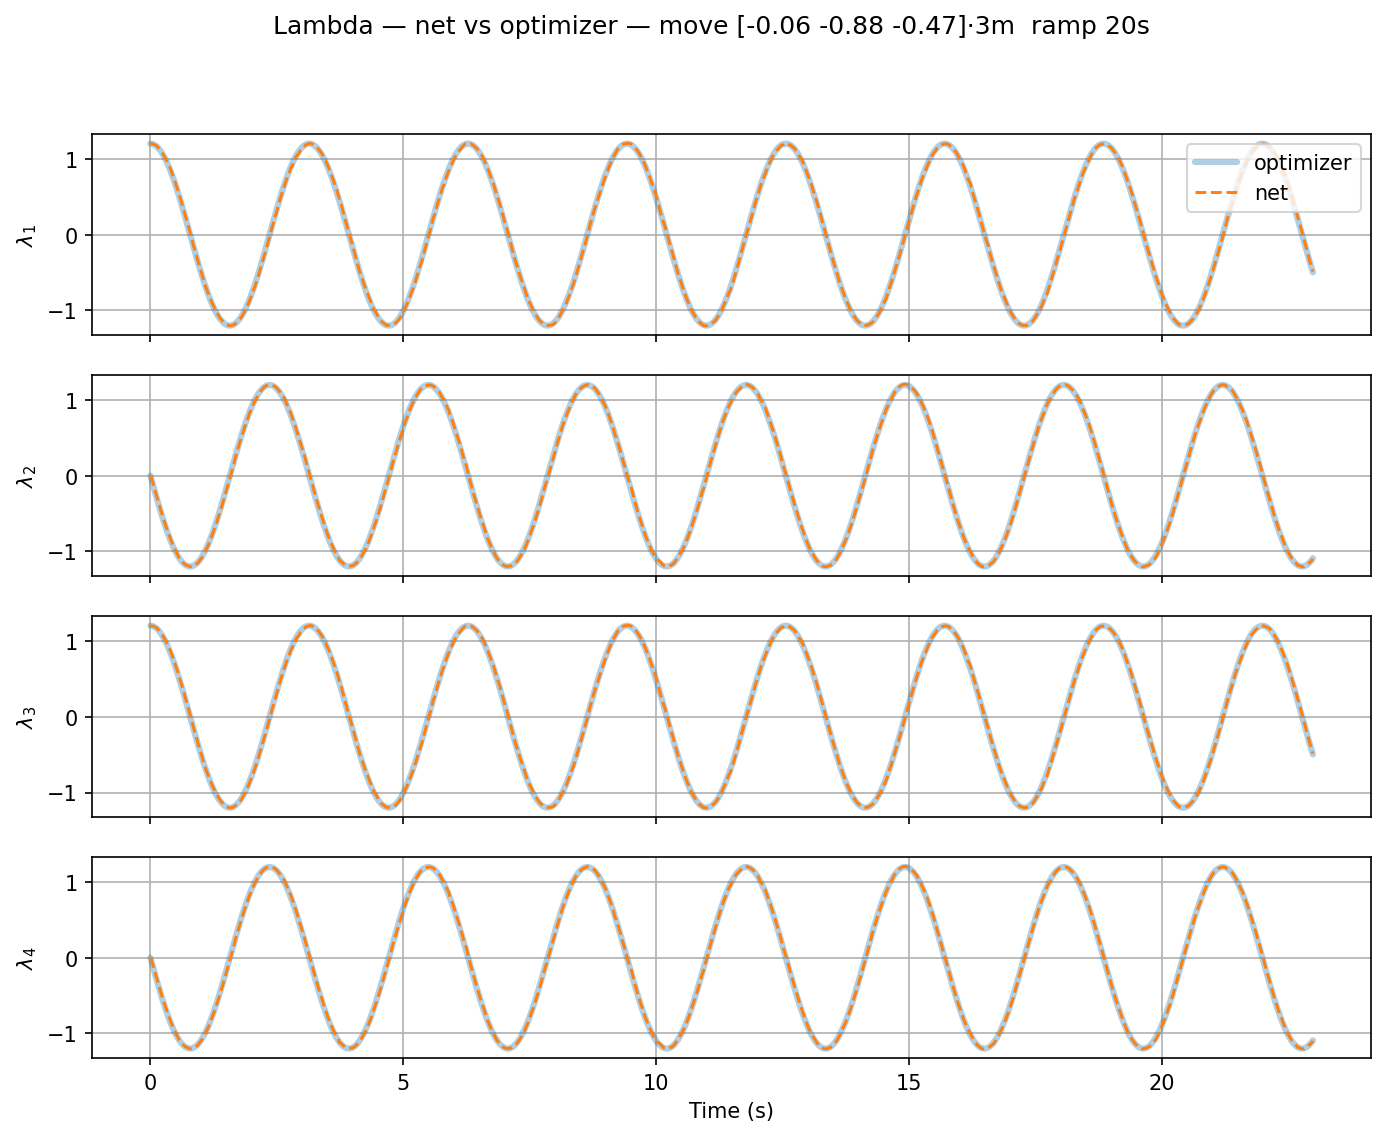
\includegraphics[width=0.8\textwidth]{figures/fig-gen-time-short-lambda.png}
  \caption{$\lambda$ produced by the network vs.\ the optimizer.}
  \label{fig:gen-time-short-lambda}
\end{figure}

\begin{figure}[H]
  \centering
  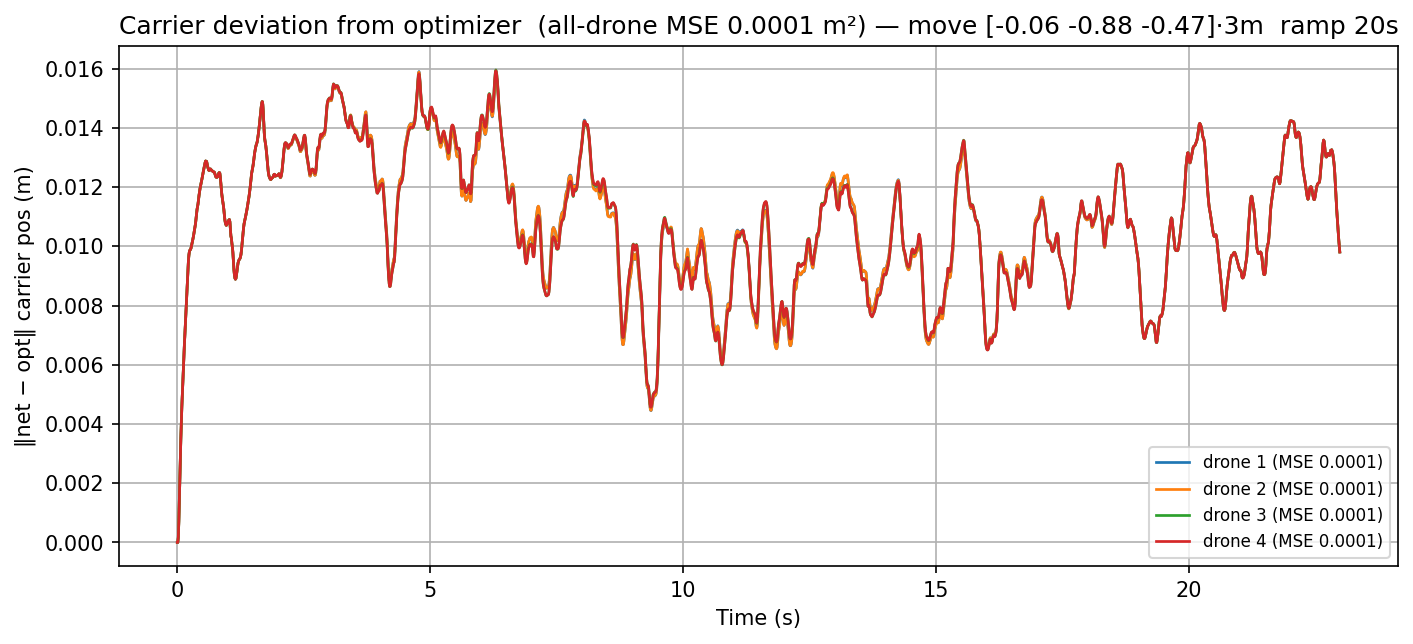
\includegraphics[width=0.8\textwidth]{figures/fig-gen-time-short-carrier-dev.png}
  \caption{Carrier deviation from the optimizer.}
  \label{fig:gen-time-short-carrier-dev}
\end{figure}

\begin{figure}[H]
  \centering
  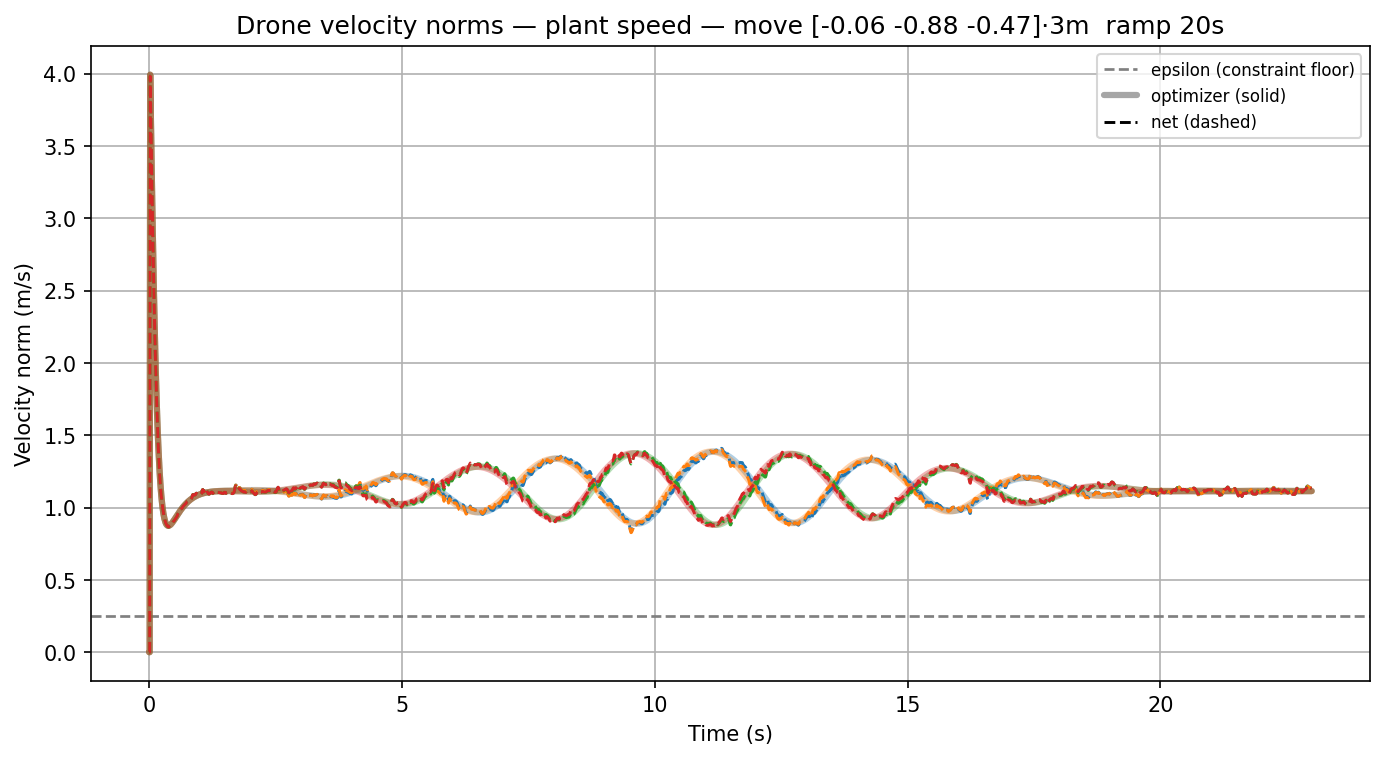
\includegraphics[width=0.8\textwidth]{figures/fig-gen-time-short-vnorms.png}
  \caption{Drone velocity norms (plant speed).}
  \label{fig:gen-time-short-vnorms}
\end{figure}

\begin{figure}[H]
  \centering
  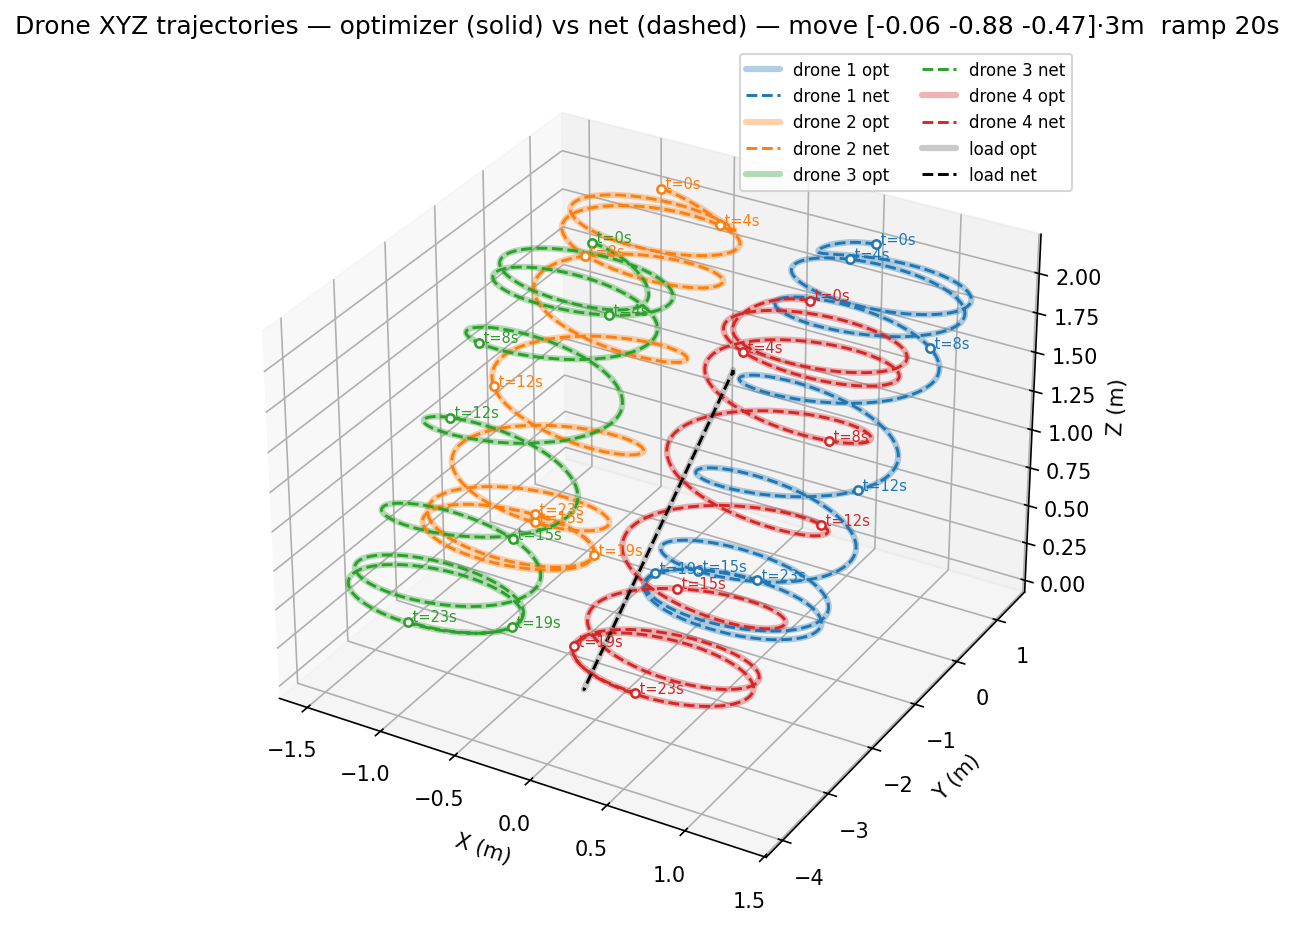
\includegraphics[width=0.8\textwidth]{figures/fig-gen-time-short-xyz.png}
  \caption{Drone XYZ trajectories: optimizer (solid) vs.\ net (dashed).}
  \label{fig:gen-time-short-xyz}
\end{figure}

\begin{table}[H]
  \centering
  \caption{Performance of the network on the shorter-time generalization trajectory.}
  \label{tab:gen-time-short}
  \begin{tabular}{lcc}
    \hline
    \textbf{Metric} & \textbf{Network} & \textbf{Optimizer} \\
    \hline
    Load tracking MSE (m$^2$) & 0.00043 & 0.00043 \\
    Load tracking max error (m) & 0.03105 & 0.03105 \\
    \hline
    \multicolumn{3}{l}{\textbf{Carrier deviation from optimizer, MSE (m$^2$)}} \\
    \hline
    Drone 1 & 0.00012 & -- \\
    Drone 2 & 0.00012 & -- \\
    Drone 3 & 0.00012 & -- \\
    Drone 4 & 0.00012 & -- \\
    All drones & 0.00012 & -- \\
    \hline
    \multicolumn{3}{l}{\textbf{$\lambda$ deviation from optimizer, MSE}} \\
    \hline
    Drone 1 & 0.00030 & -- \\
    Drone 2 & 0.00032 & -- \\
    Drone 3 & 0.00030 & -- \\
    Drone 4 & 0.00032 & -- \\
    All drones & 0.00031 & -- \\
    \hline
  \end{tabular}
\end{table}

\subsubsection{Generalization across distances}

\noindent\textbf{Larger-magnitude trajectory (move $[-0.06, -0.88, -0.47]\cdot15$\,m, ramp, 70\,s)}

\begin{figure}[H]
  \centering
  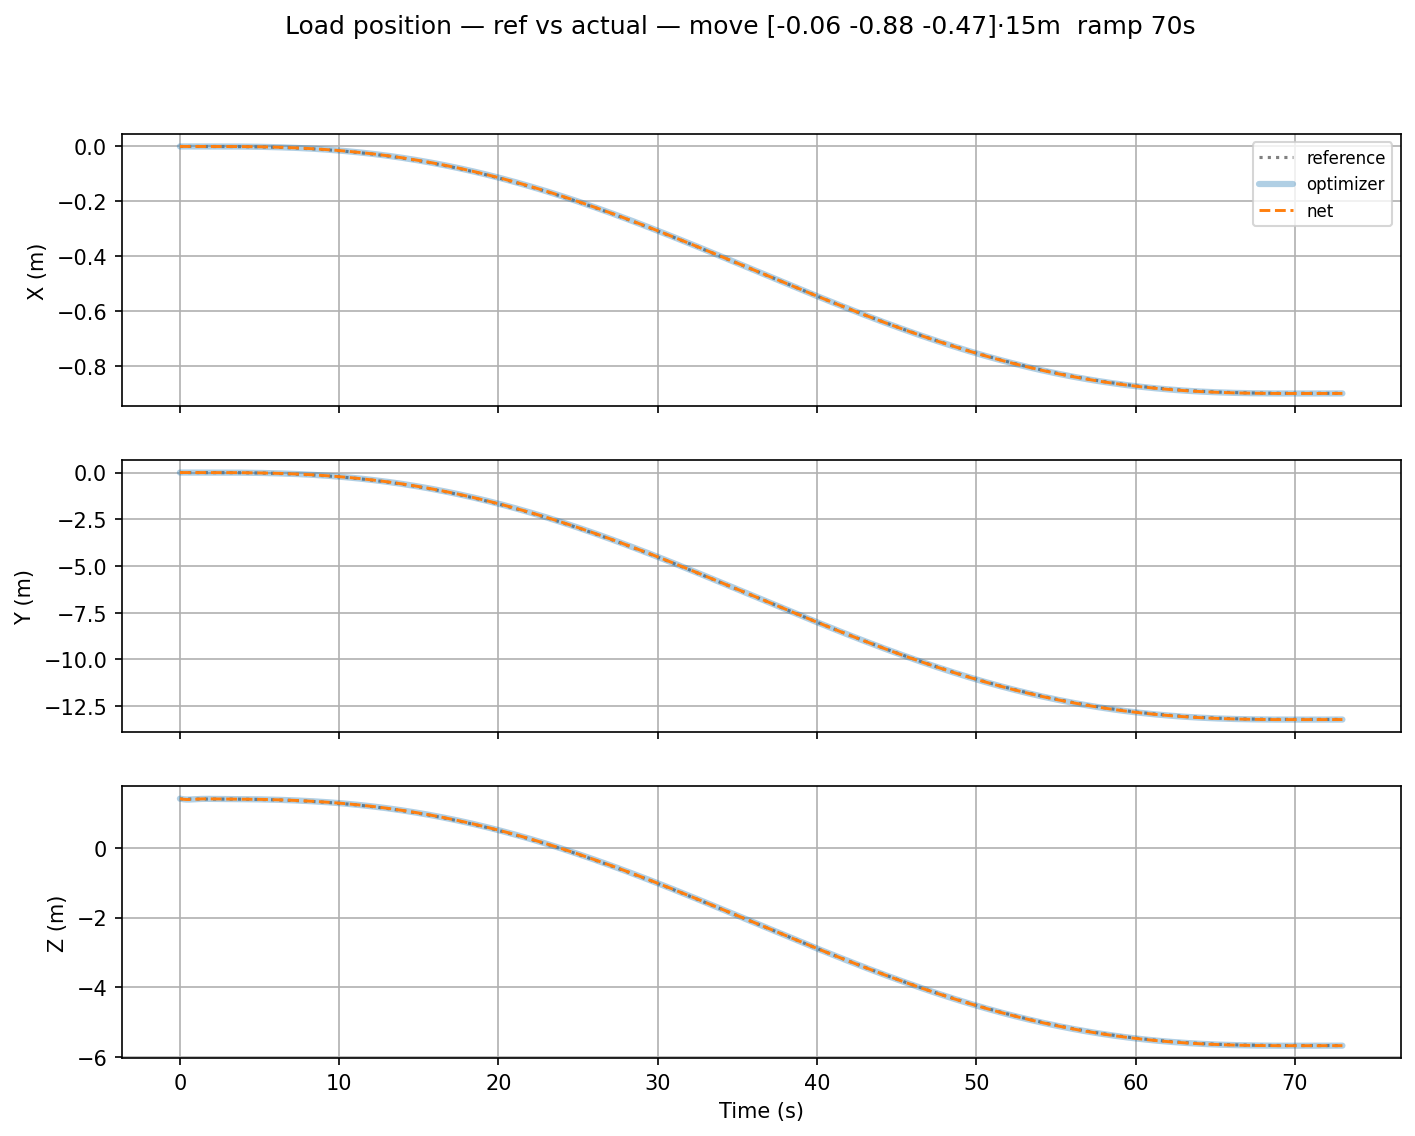
\includegraphics[width=0.8\textwidth]{figures/fig-gen-mag-load-pos.png}
  \caption{Load position: reference vs.\ actual.}
  \label{fig:gen-mag-load-pos}
\end{figure}

\begin{figure}[H]
  \centering
  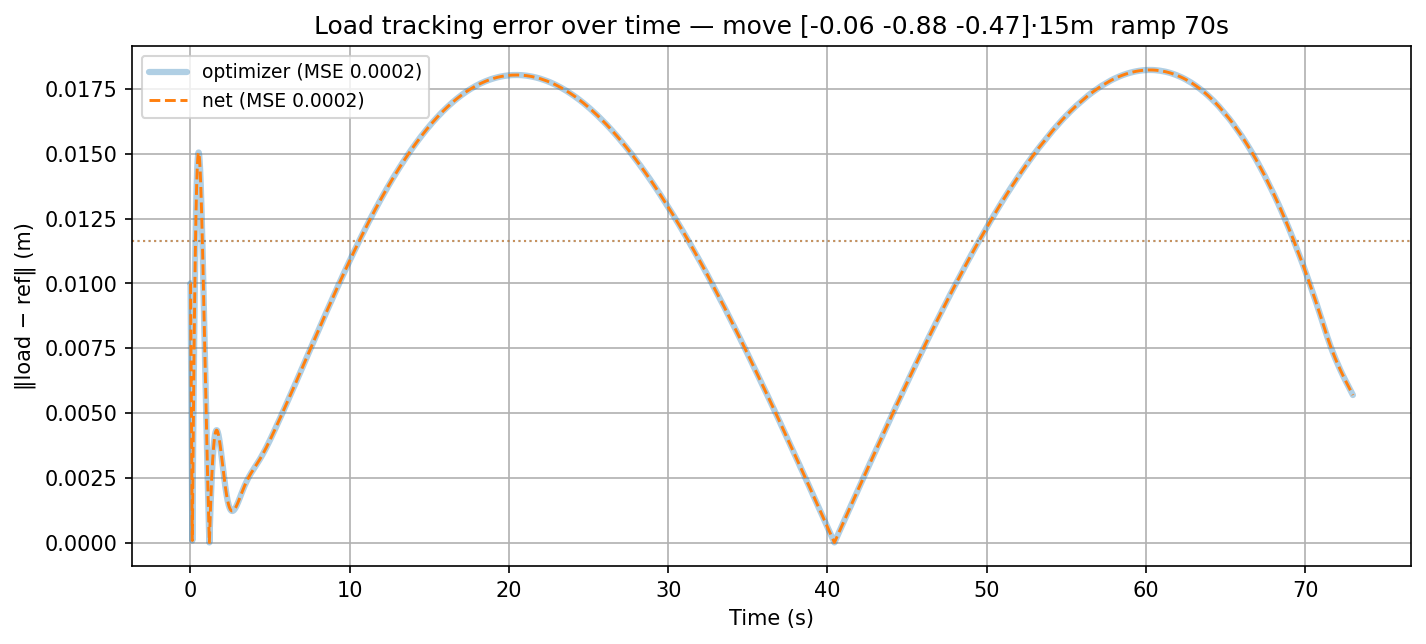
\includegraphics[width=0.8\textwidth]{figures/fig-gen-mag-load-err.png}
  \caption{Load tracking error over time.}
  \label{fig:gen-mag-load-err}
\end{figure}

\begin{figure}[H]
  \centering
  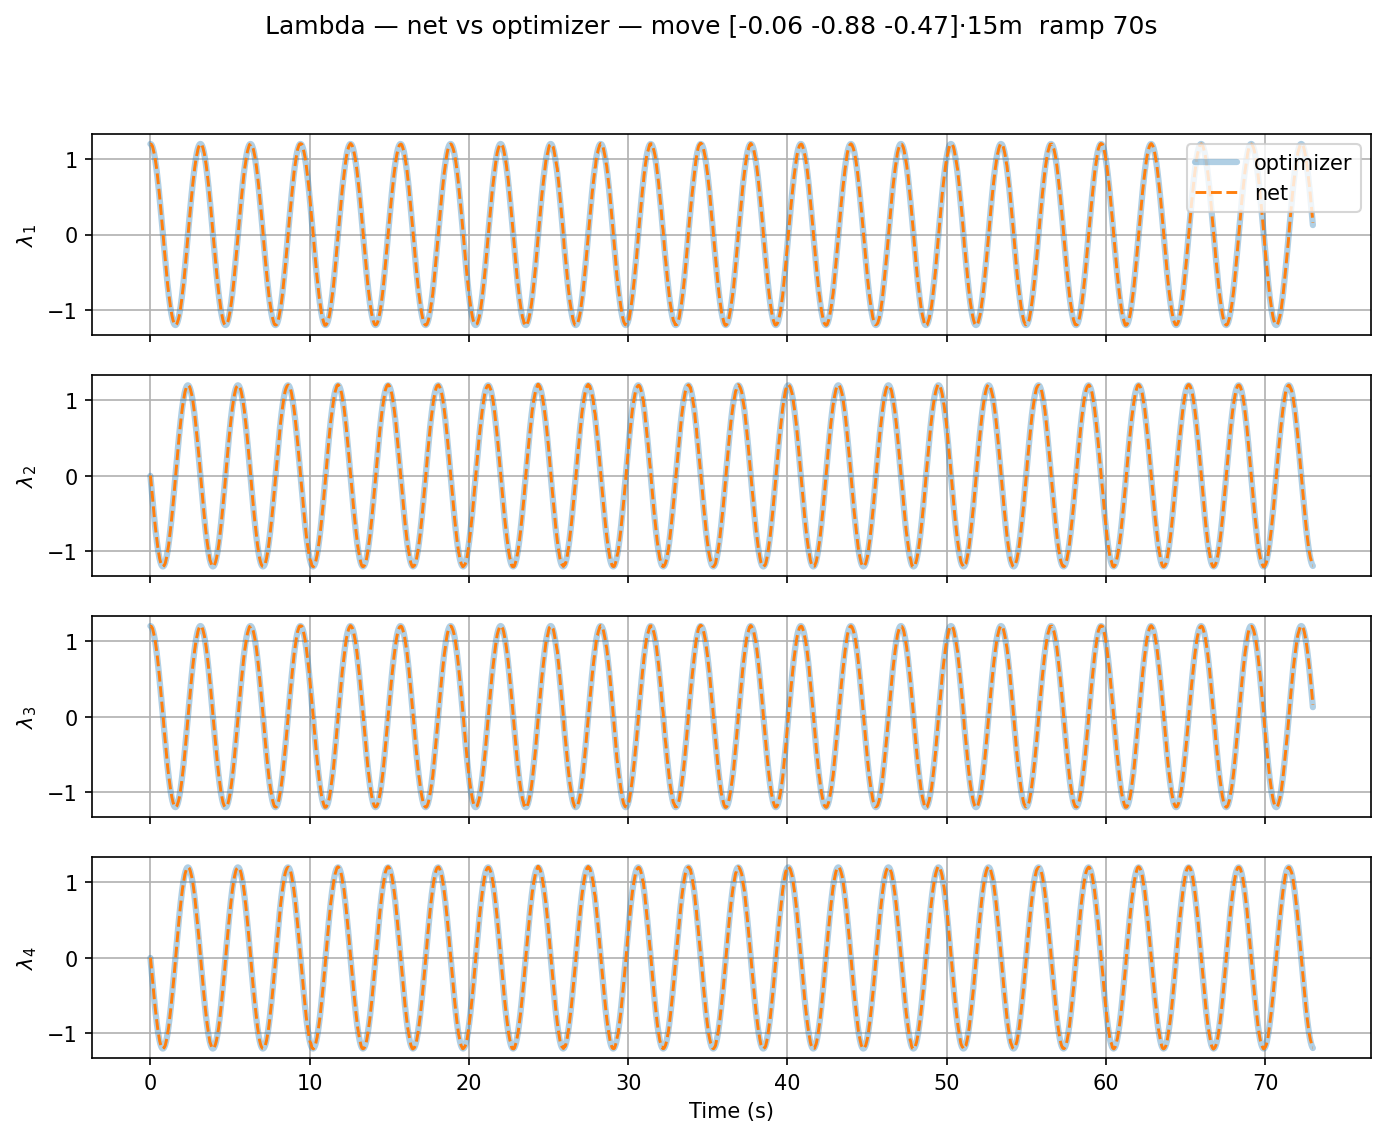
\includegraphics[width=0.8\textwidth]{figures/fig-gen-mag-lambda.png}
  \caption{$\lambda$ produced by the network vs.\ the optimizer.}
  \label{fig:gen-mag-lambda}
\end{figure}

\begin{figure}[H]
  \centering
  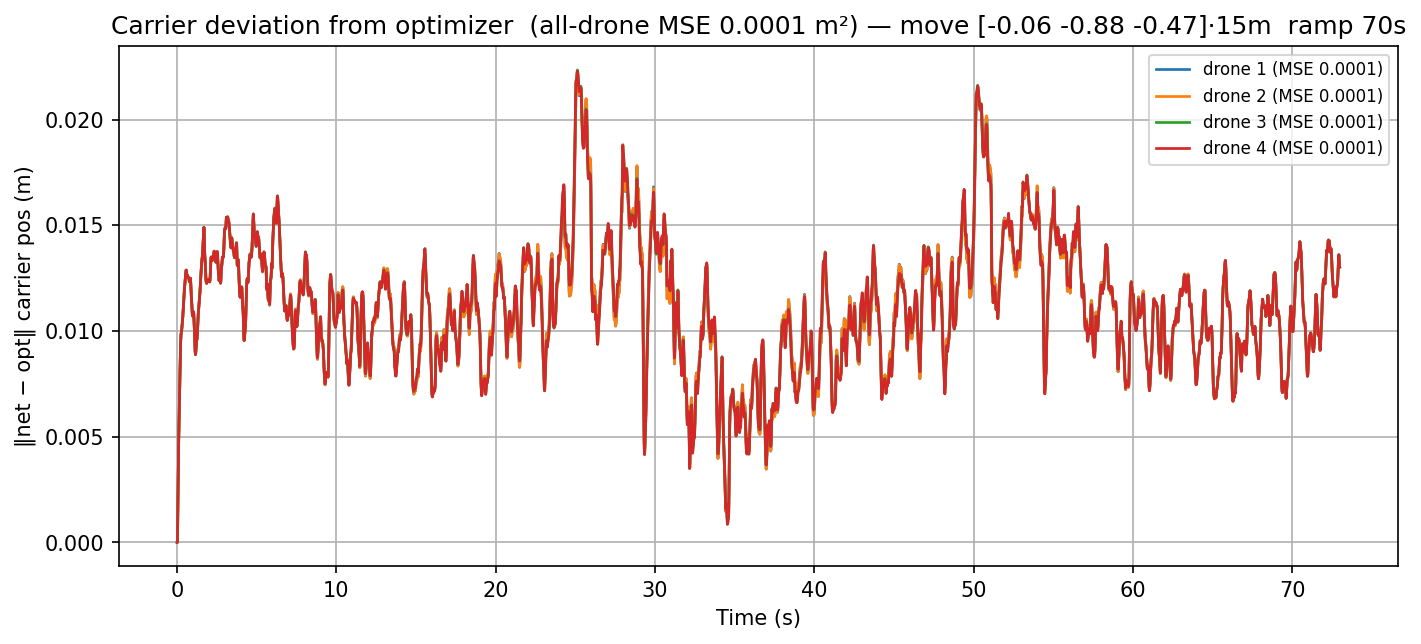
\includegraphics[width=0.8\textwidth]{figures/fig-gen-mag-carrier-dev.png}
  \caption{Carrier deviation from the optimizer.}
  \label{fig:gen-mag-carrier-dev}
\end{figure}

\begin{figure}[H]
  \centering
  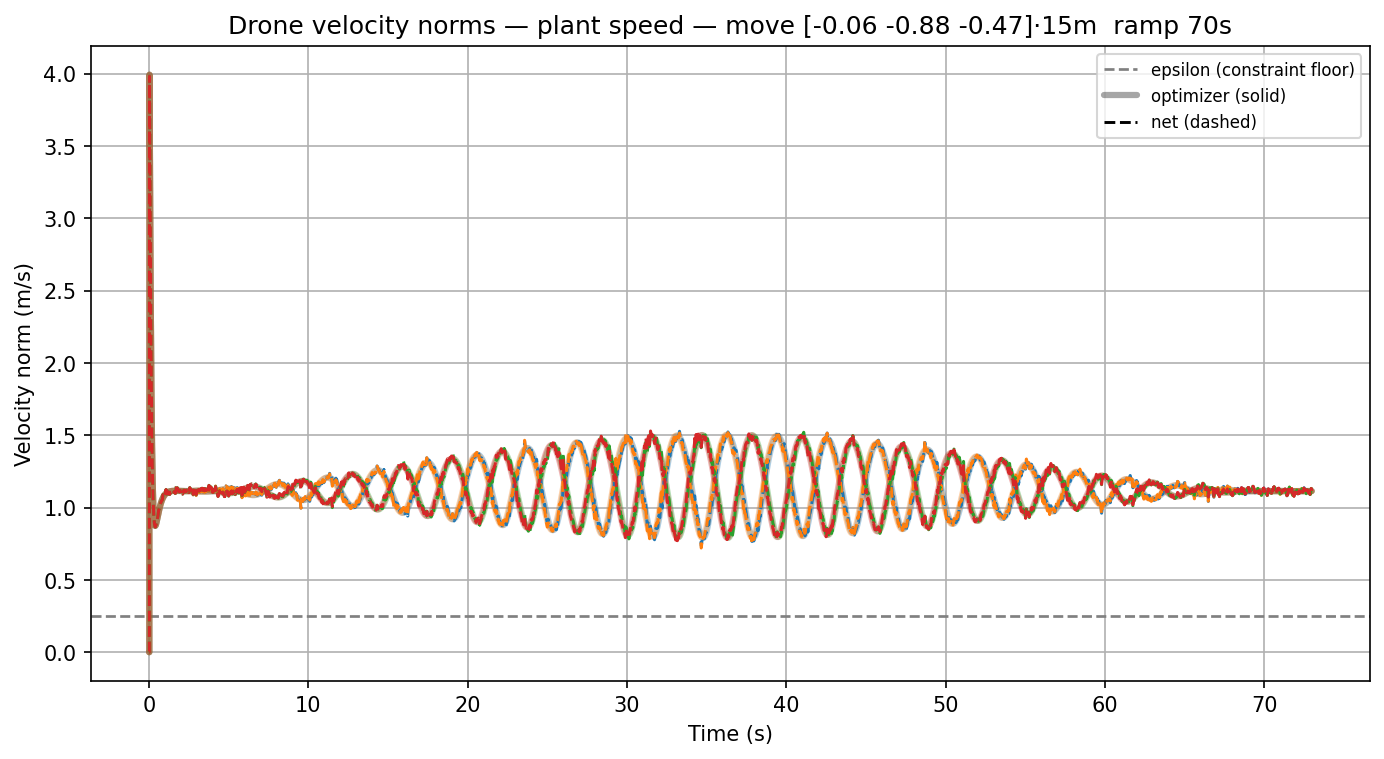
\includegraphics[width=0.8\textwidth]{figures/fig-gen-mag-vnorms.png}
  \caption{Drone velocity norms (plant speed).}
  \label{fig:gen-mag-vnorms}
\end{figure}

\begin{figure}[H]
  \centering
  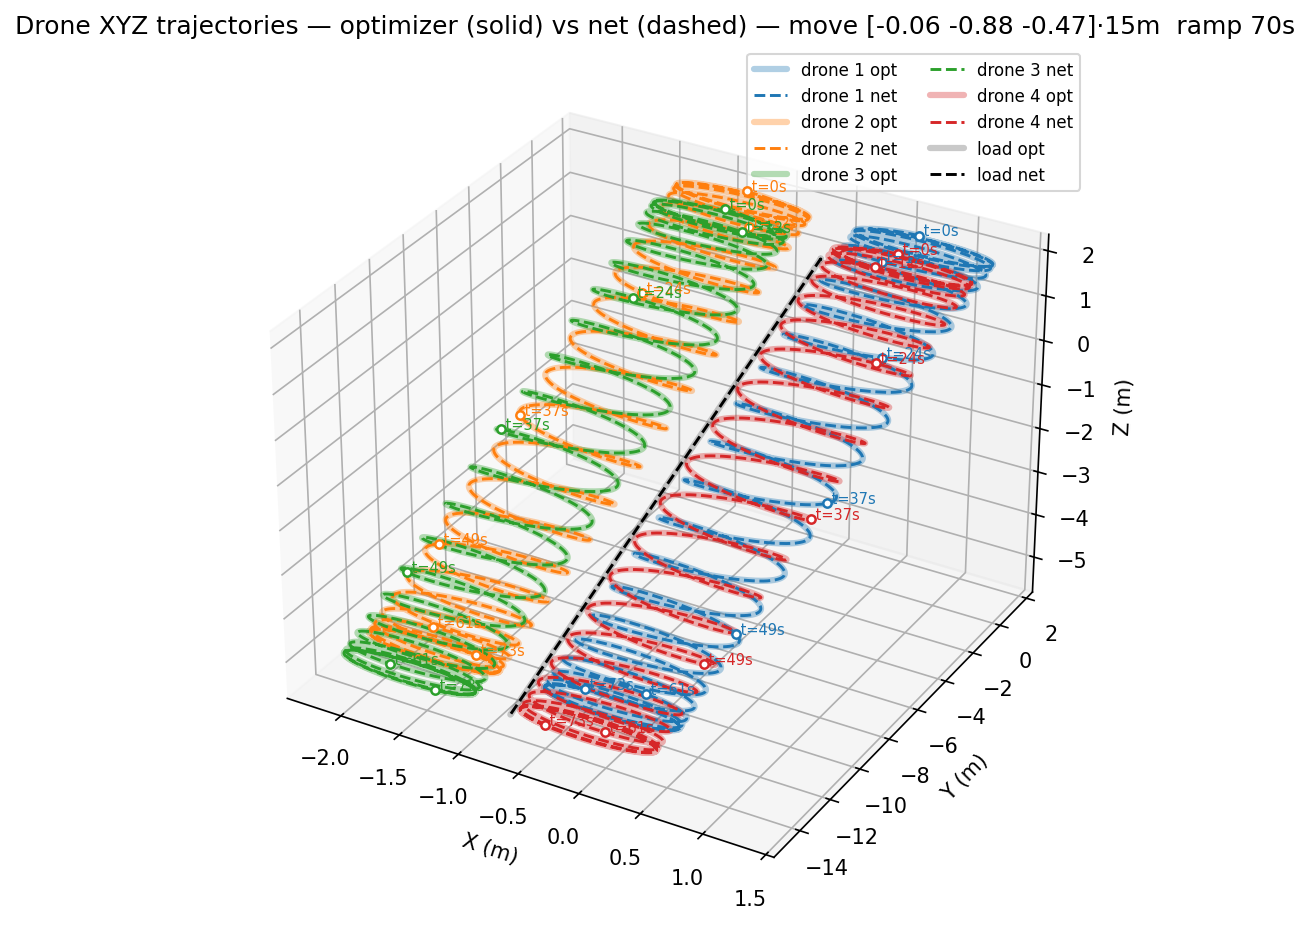
\includegraphics[width=0.8\textwidth]{figures/fig-gen-mag-xyz.png}
  \caption{Drone XYZ trajectories: optimizer (solid) vs.\ net (dashed).}
  \label{fig:gen-mag-xyz}
\end{figure}

\begin{figure}[H]
  \centering
  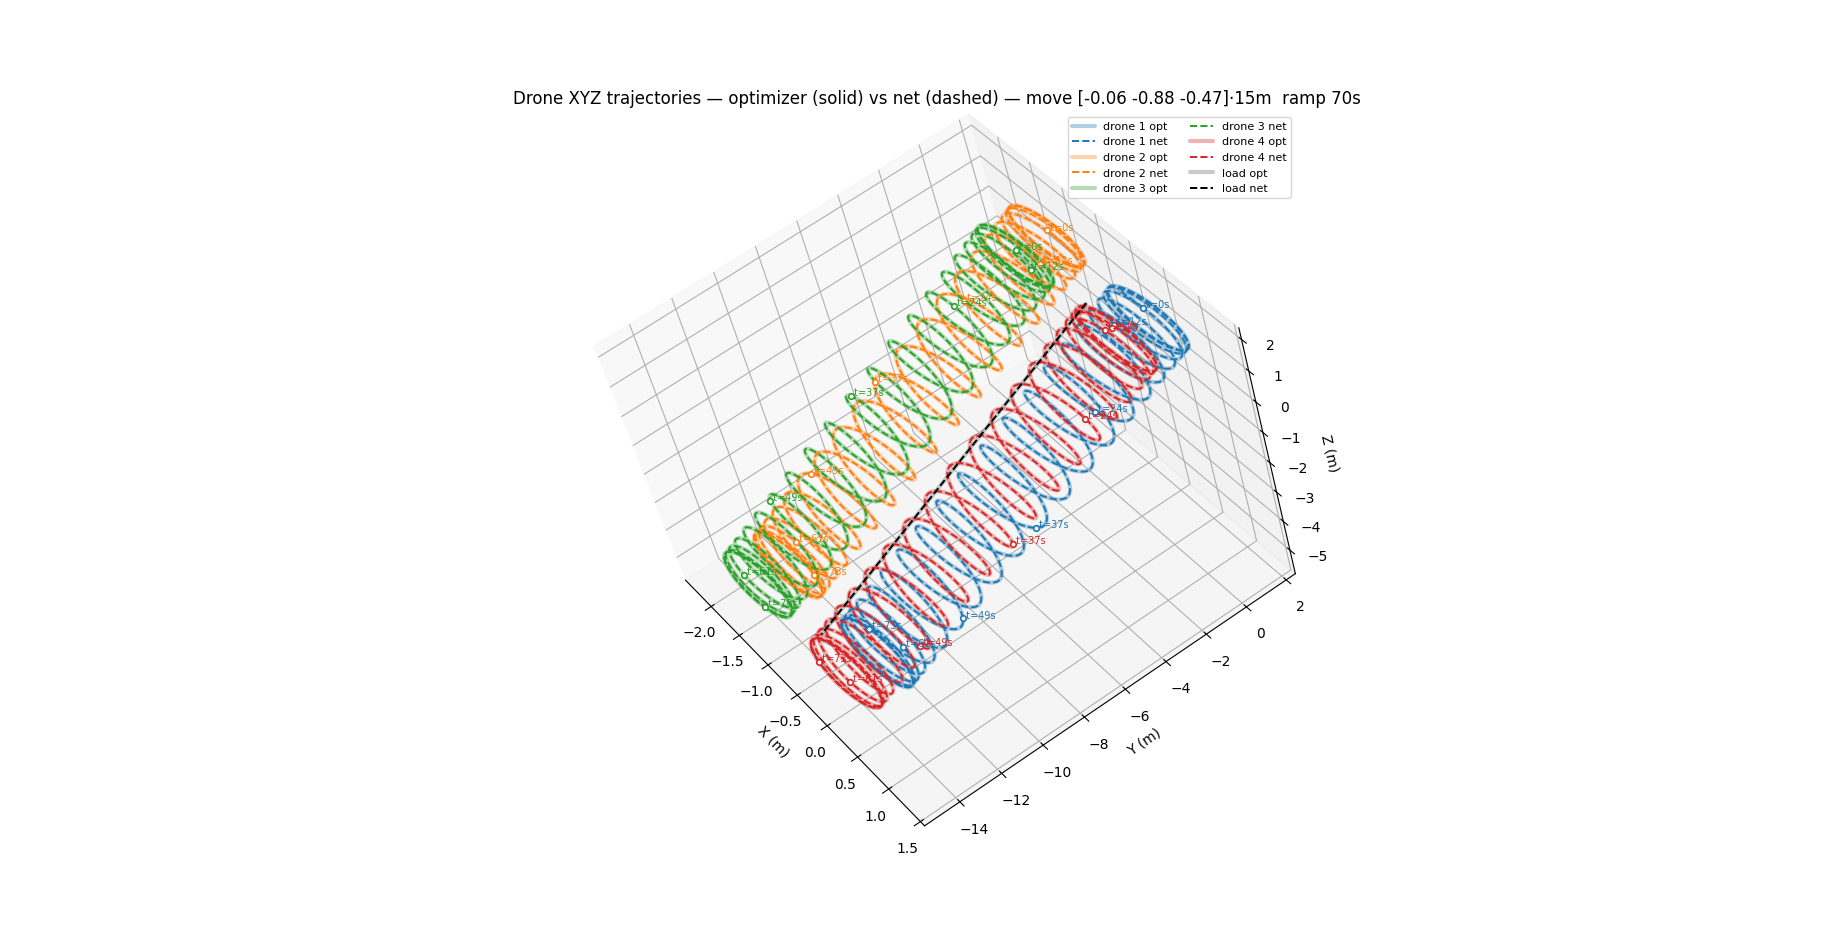
\includegraphics[width=\textwidth]{figures/fig-gen-mag-xyz-2ndpov.png}
  \caption{Drone XYZ trajectories, second point of view: optimizer (solid) vs.\ net (dashed).}
  \label{fig:gen-mag-xyz-2ndpov}
\end{figure}

\begin{table}[H]
  \centering
  \caption{Performance of the network on the larger-magnitude generalization trajectory.}
  \label{tab:gen-mag}
  \begin{tabular}{lcc}
    \hline
    \textbf{Metric} & \textbf{Network} & \textbf{Optimizer} \\
    \hline
    Load tracking MSE (m$^2$) & 0.00017 & 0.00017 \\
    Load tracking max error (m) & 0.01824 & 0.01824 \\
    \hline
    \multicolumn{3}{l}{\textbf{Carrier deviation from optimizer, MSE (m$^2$)}} \\
    \hline
    Drone 1 & 0.00013 & -- \\
    Drone 2 & 0.00013 & -- \\
    Drone 3 & 0.00013 & -- \\
    Drone 4 & 0.00013 & -- \\
    All drones & 0.00013 & -- \\
    \hline
    \multicolumn{3}{l}{\textbf{$\lambda$ deviation from optimizer, MSE}} \\
    \hline
    Drone 1 & 0.00032 & -- \\
    Drone 2 & 0.00036 & -- \\
    Drone 3 & 0.00032 & -- \\
    Drone 4 & 0.00036 & -- \\
    All drones & 0.00034 & -- \\
    \hline
  \end{tabular}
\end{table}

\subsubsection{Generalization across directions}

\noindent\textbf{Direction 1 (move $[-0.5, -1, 0.5]\cdot5$\,m, ramp, 30\,s)}

\begin{figure}[H]
  \centering
  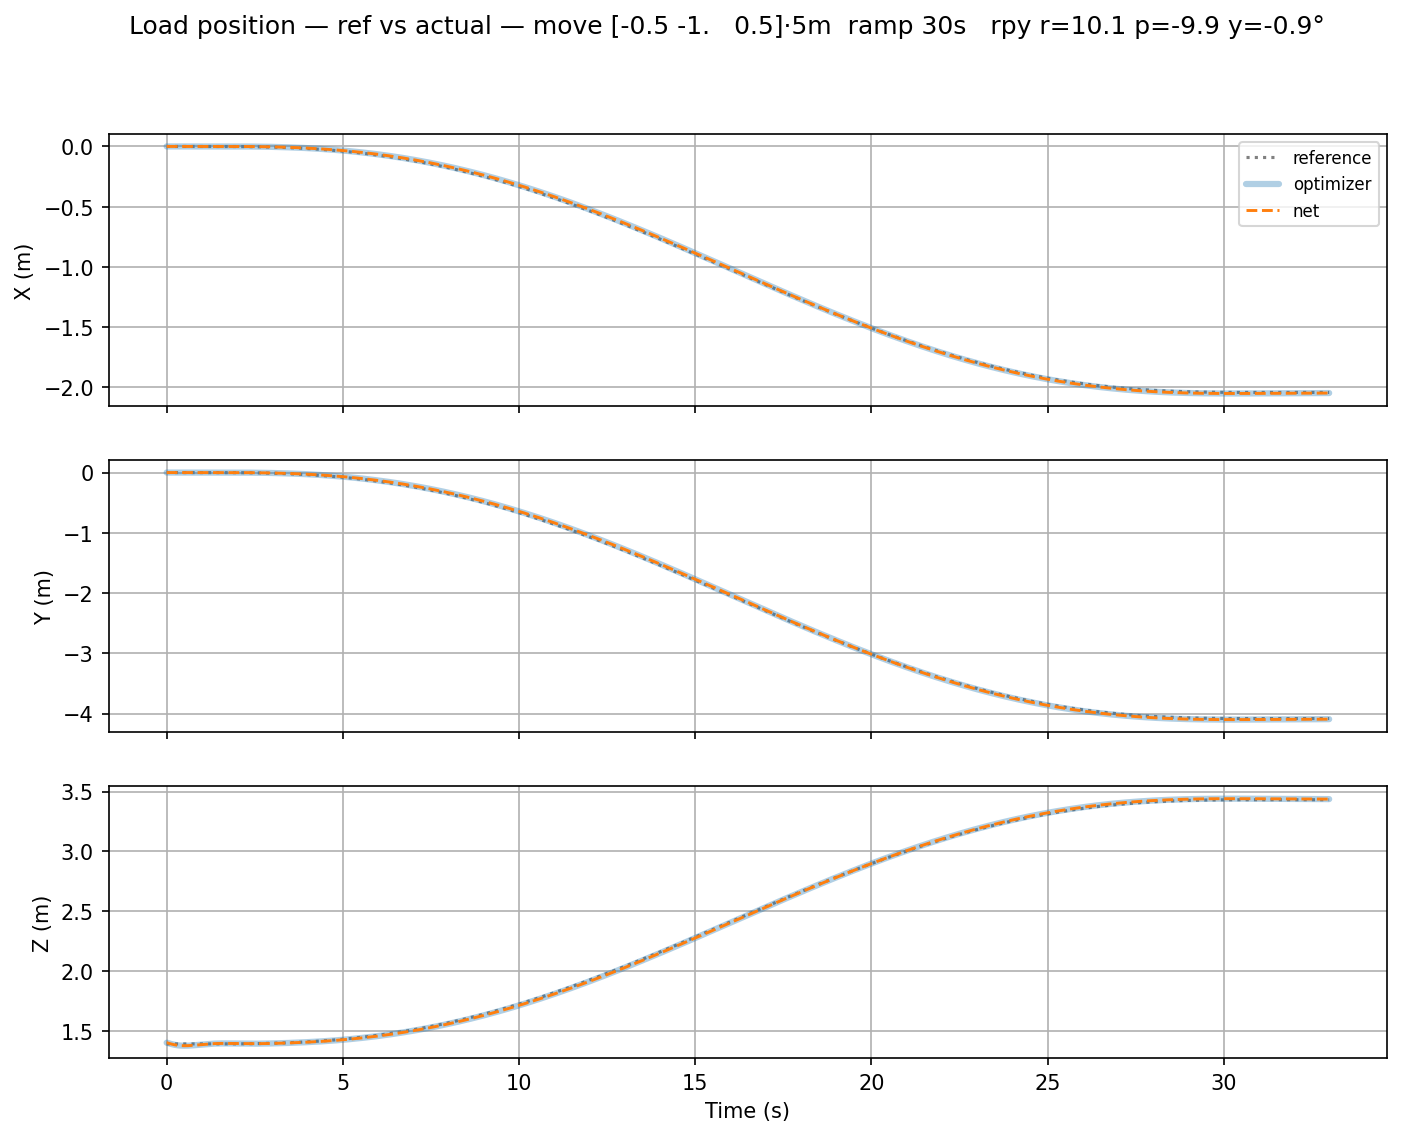
\includegraphics[width=0.8\textwidth]{figures/fig-gen-dir1-load-pos.png}
  \caption{Load position: reference vs.\ actual.}
  \label{fig:gen-dir1-load-pos}
\end{figure}

\begin{figure}[H]
  \centering
  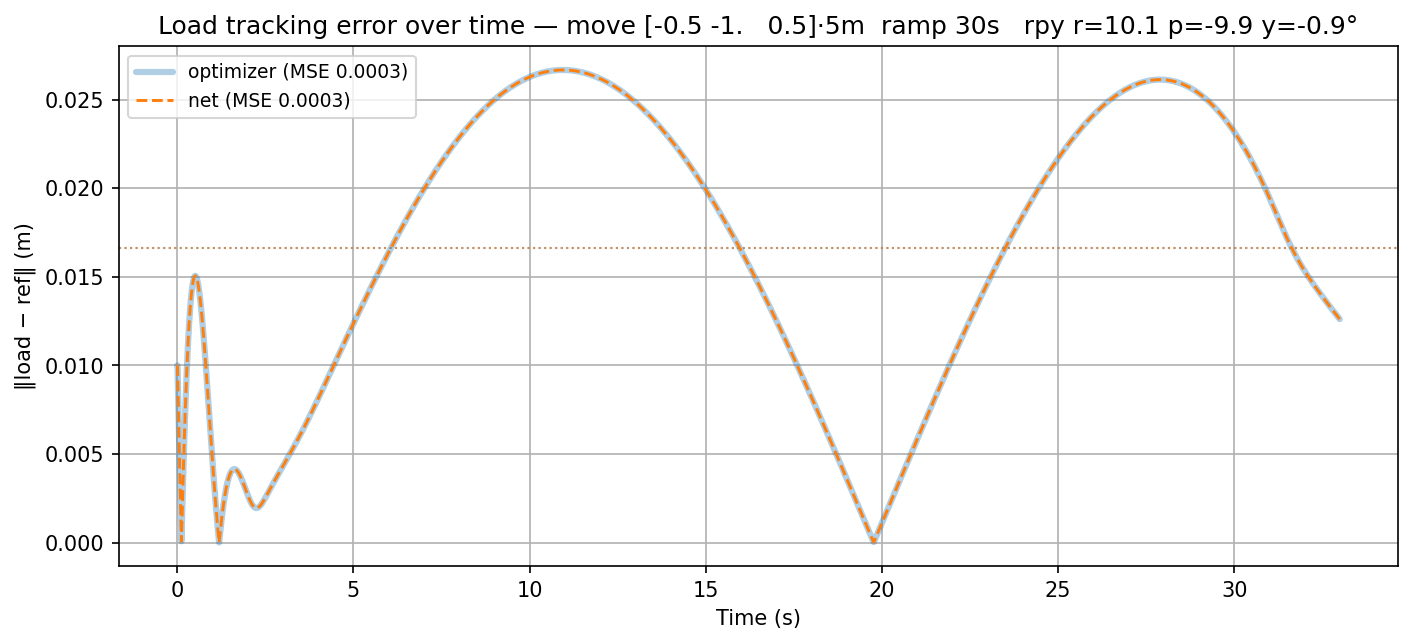
\includegraphics[width=0.8\textwidth]{figures/fig-gen-dir1-load-err.png}
  \caption{Load tracking error over time.}
  \label{fig:gen-dir1-load-err}
\end{figure}

\begin{figure}[H]
  \centering
  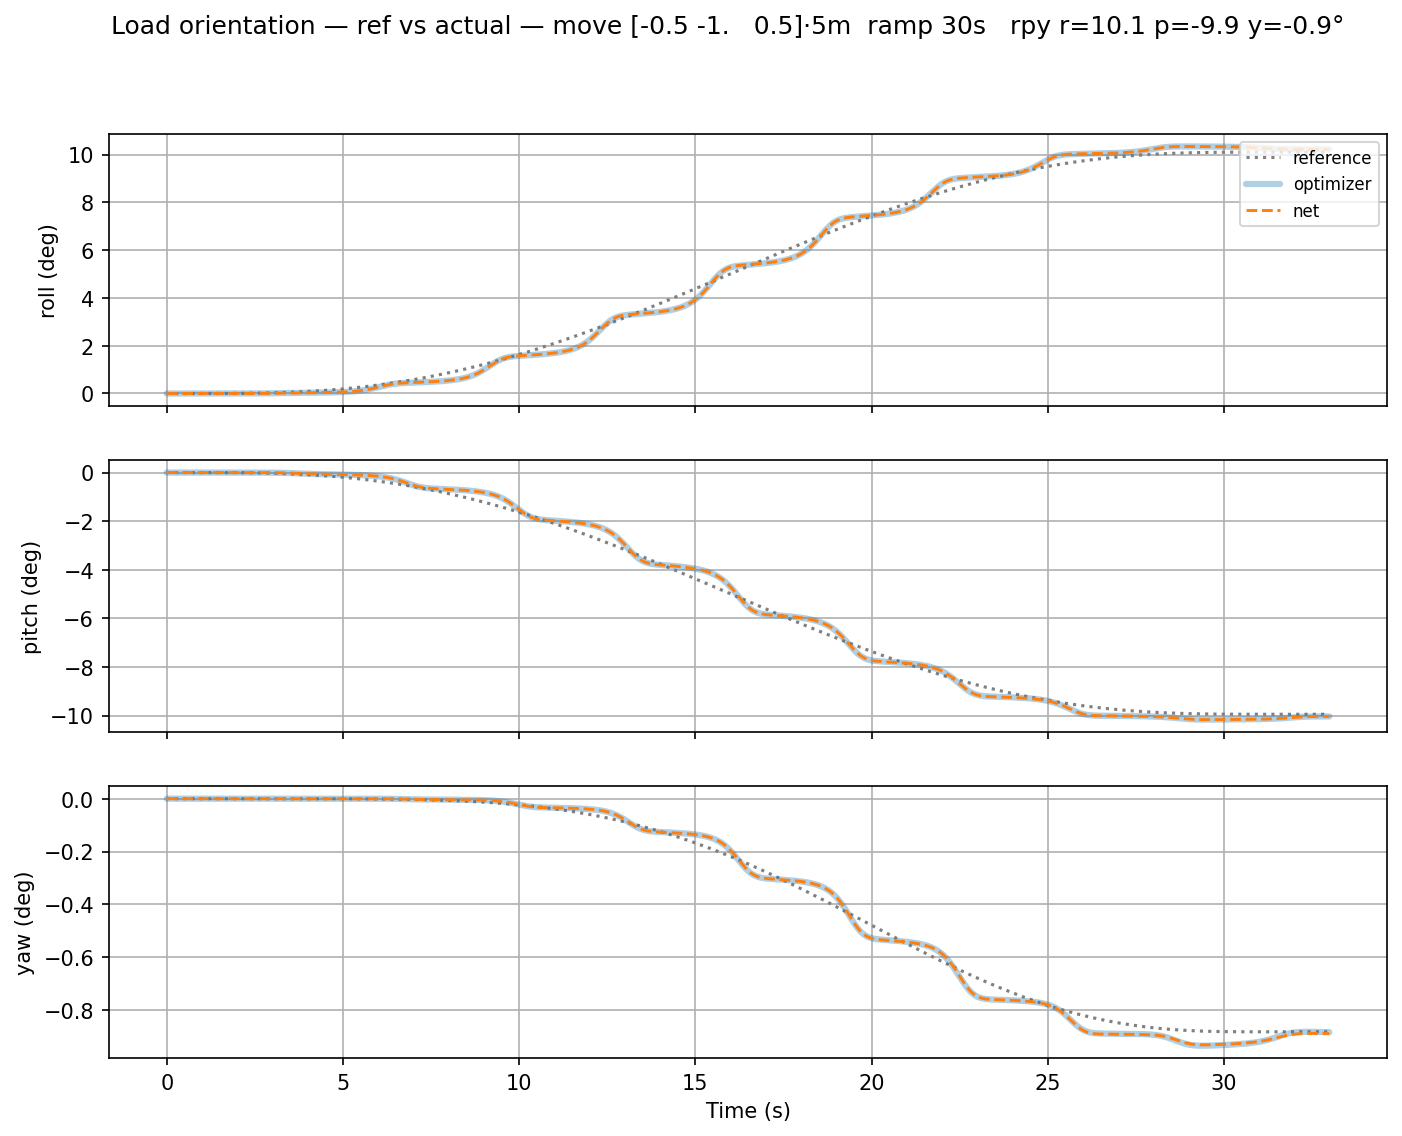
\includegraphics[width=0.8\textwidth]{figures/fig-gen-dir1-load-orient.png}
  \caption{Load orientation: reference vs.\ actual.}
  \label{fig:gen-dir1-load-orient}
\end{figure}

\begin{figure}[H]
  \centering
  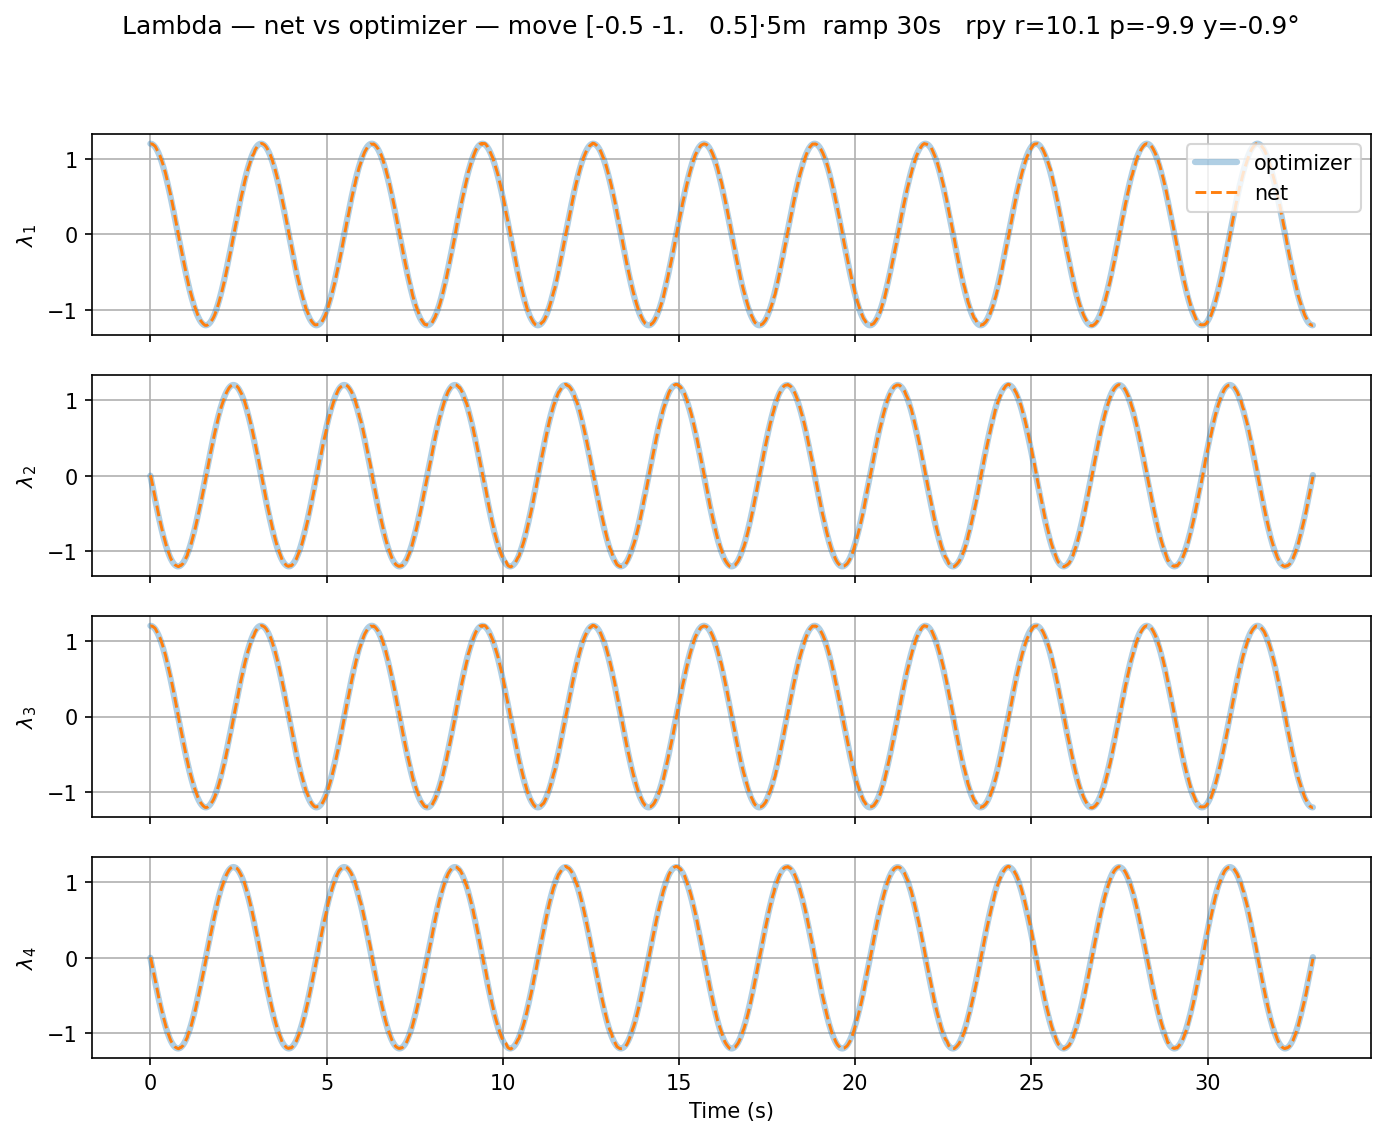
\includegraphics[width=0.8\textwidth]{figures/fig-gen-dir1-lambda.png}
  \caption{$\lambda$ produced by the network vs.\ the optimizer.}
  \label{fig:gen-dir1-lambda}
\end{figure}

\begin{figure}[H]
  \centering
  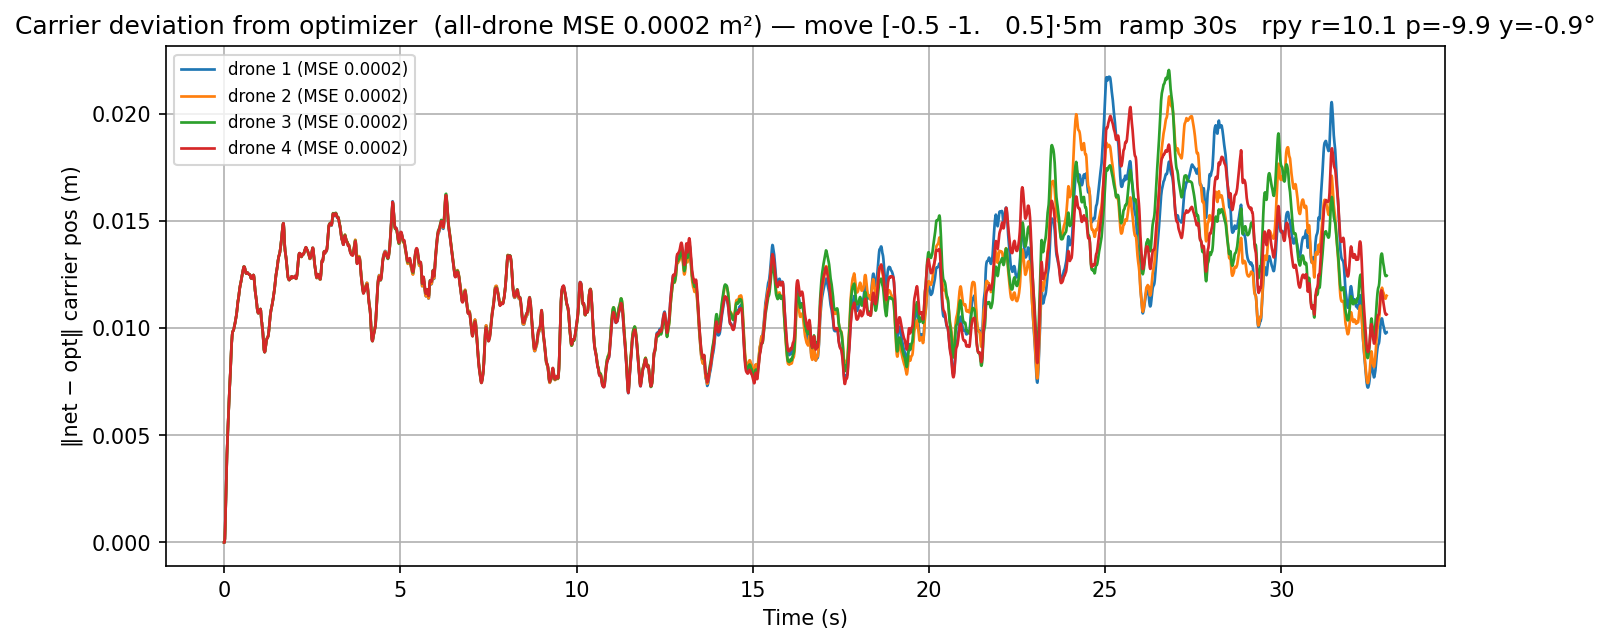
\includegraphics[width=0.8\textwidth]{figures/fig-gen-dir1-carrier-dev.png}
  \caption{Carrier deviation from the optimizer.}
  \label{fig:gen-dir1-carrier-dev}
\end{figure}

\begin{figure}[H]
  \centering
  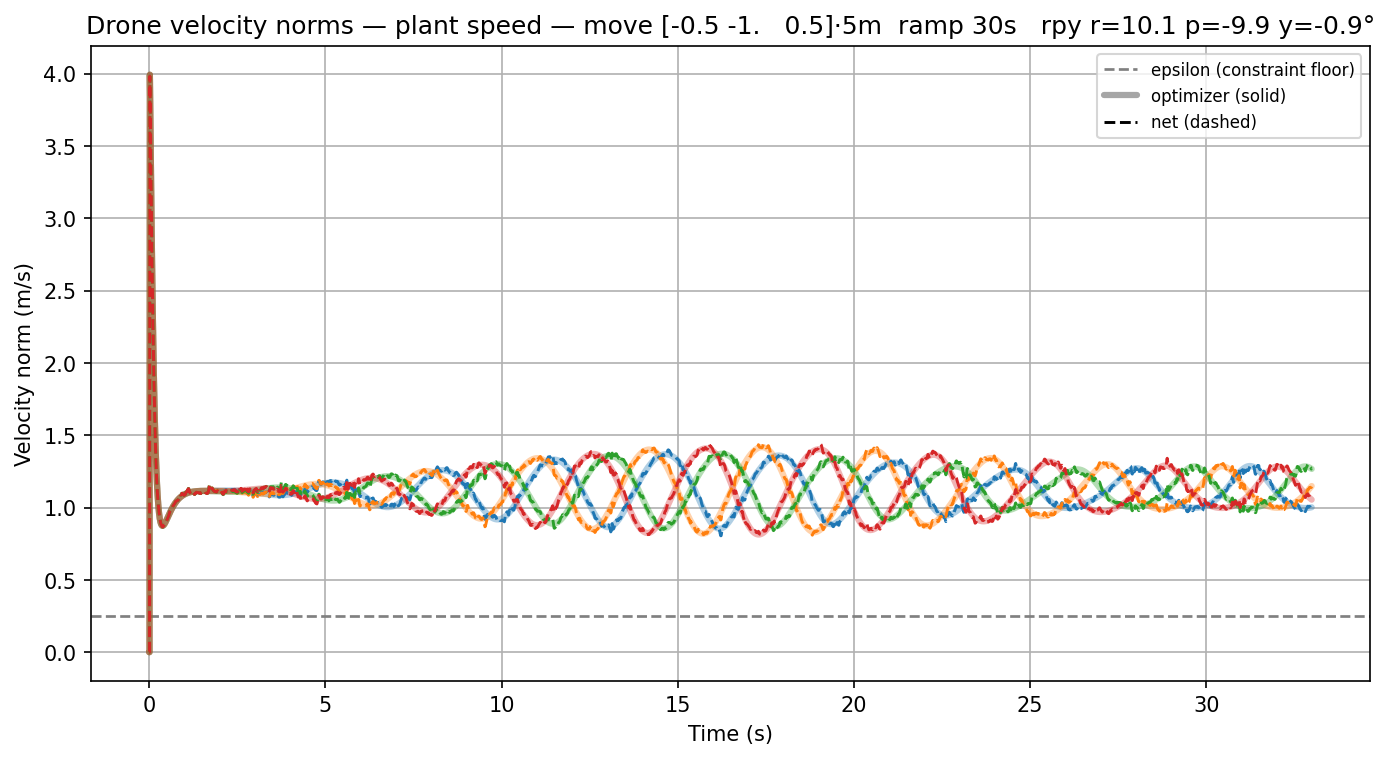
\includegraphics[width=0.8\textwidth]{figures/fig-gen-dir1-vnorms.png}
  \caption{Drone velocity norms (plant speed).}
  \label{fig:gen-dir1-vnorms}
\end{figure}

\begin{figure}[H]
  \centering
  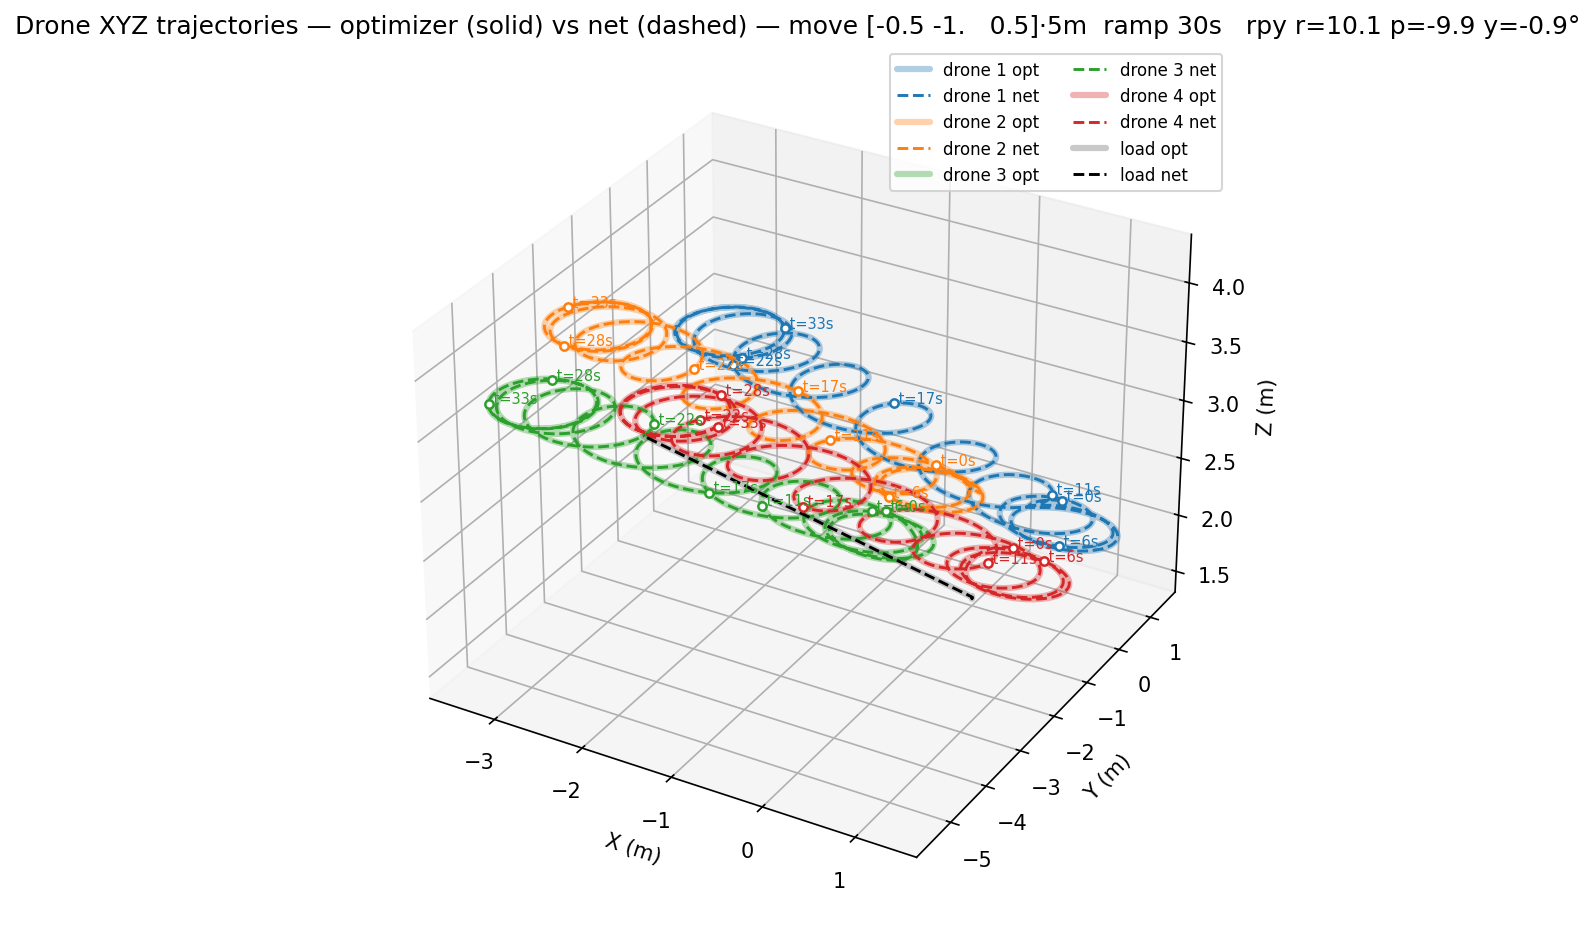
\includegraphics[width=0.8\textwidth]{figures/fig-gen-dir1-xyz.png}
  \caption{Drone XYZ trajectories: optimizer (solid) vs.\ net (dashed).}
  \label{fig:gen-dir1-xyz}
\end{figure}

\begin{table}[H]
  \centering
  \caption{Performance of the network on generalization direction 1.}
  \label{tab:gen-dir1}
  \begin{tabular}{lcc}
    \hline
    \textbf{Metric} & \textbf{Network} & \textbf{Optimizer} \\
    \hline
    Load tracking MSE (m$^2$) & 0.00034 & 0.00034 \\
    Load tracking max error (m) & 0.02667 & 0.02667 \\
    \hline
    \multicolumn{3}{l}{\textbf{Carrier deviation from optimizer, MSE (m$^2$)}} \\
    \hline
    Drone 1 & 0.00016 & -- \\
    Drone 2 & 0.00016 & -- \\
    Drone 3 & 0.00016 & -- \\
    Drone 4 & 0.00016 & -- \\
    All drones & 0.00016 & -- \\
    \hline
    \multicolumn{3}{l}{\textbf{$\lambda$ deviation from optimizer, MSE}} \\
    \hline
    Drone 1 & 0.00037 & -- \\
    Drone 2 & 0.00042 & -- \\
    Drone 3 & 0.00037 & -- \\
    Drone 4 & 0.00042 & -- \\
    All drones & 0.00040 & -- \\
    \hline
  \end{tabular}
\end{table}

\noindent\textbf{Direction 2 (move $[0.1, 0.1, -1]\cdot5$\,m, ramp, 30\,s)}

\begin{figure}[H]
  \centering
  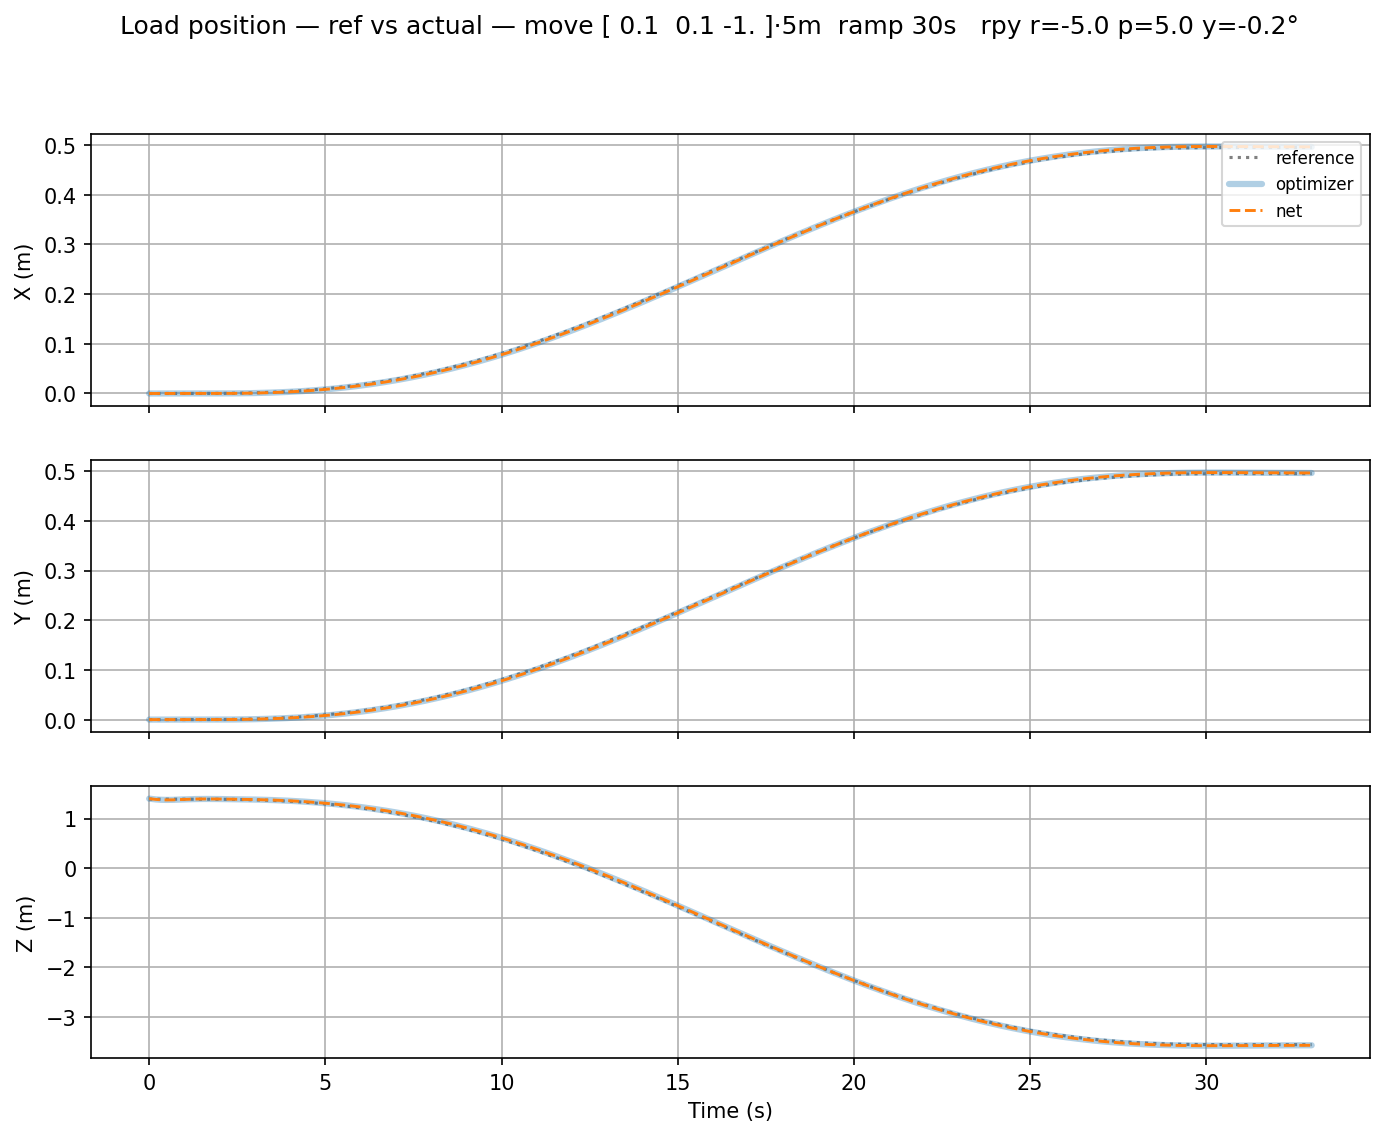
\includegraphics[width=0.8\textwidth]{figures/fig-gen-dir2-load-pos.png}
  \caption{Load position: reference vs.\ actual.}
  \label{fig:gen-dir2-load-pos}
\end{figure}

\begin{figure}[H]
  \centering
  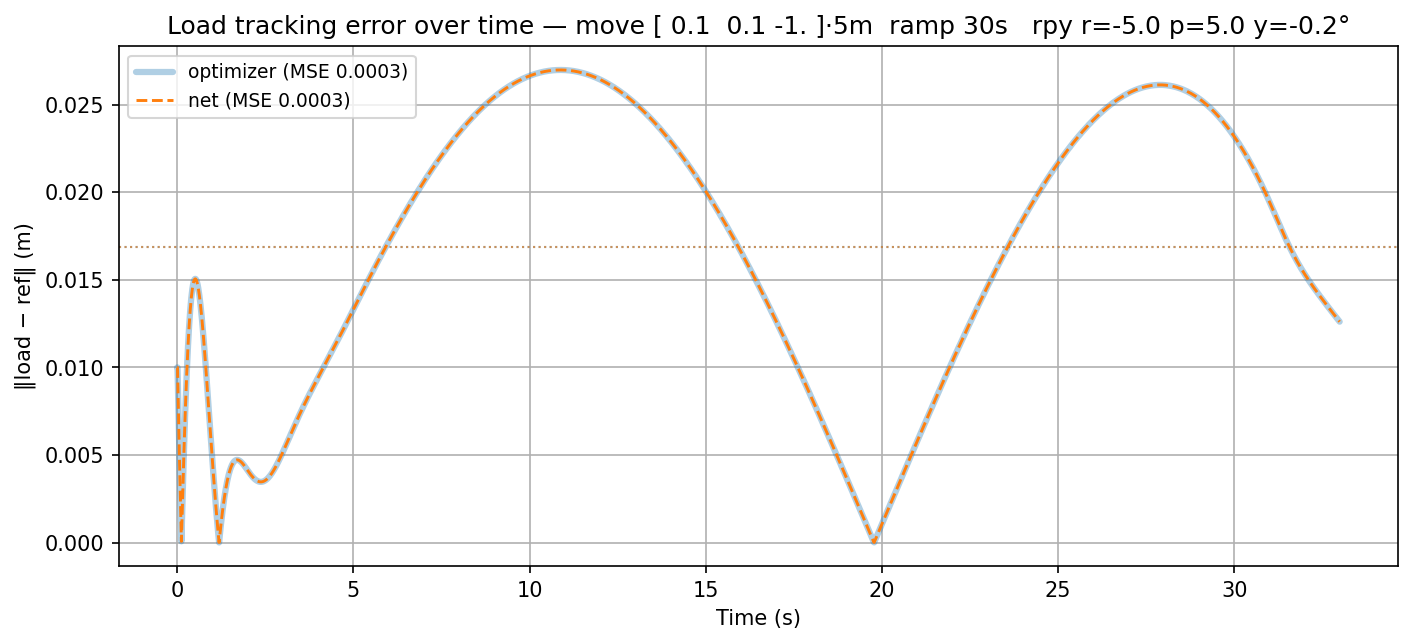
\includegraphics[width=0.8\textwidth]{figures/fig-gen-dir2-load-err.png}
  \caption{Load tracking error over time.}
  \label{fig:gen-dir2-load-err}
\end{figure}

\begin{figure}[H]
  \centering
  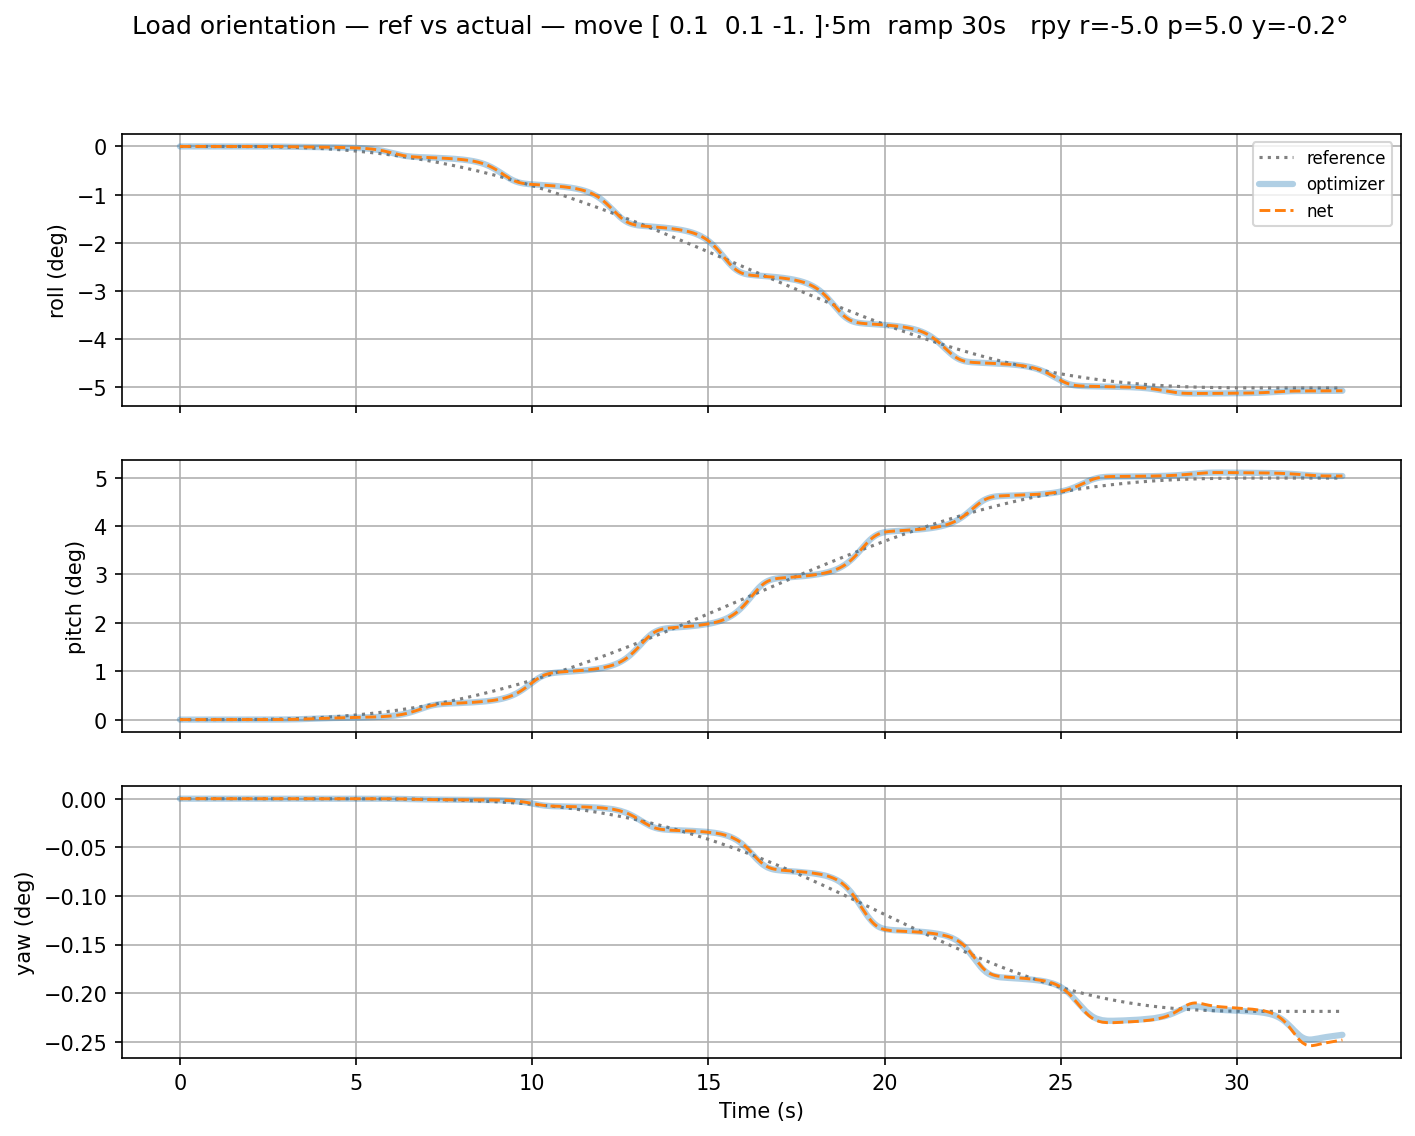
\includegraphics[width=0.8\textwidth]{figures/fig-gen-dir2-load-orient.png}
  \caption{Load orientation: reference vs.\ actual.}
  \label{fig:gen-dir2-load-orient}
\end{figure}

\begin{figure}[H]
  \centering
  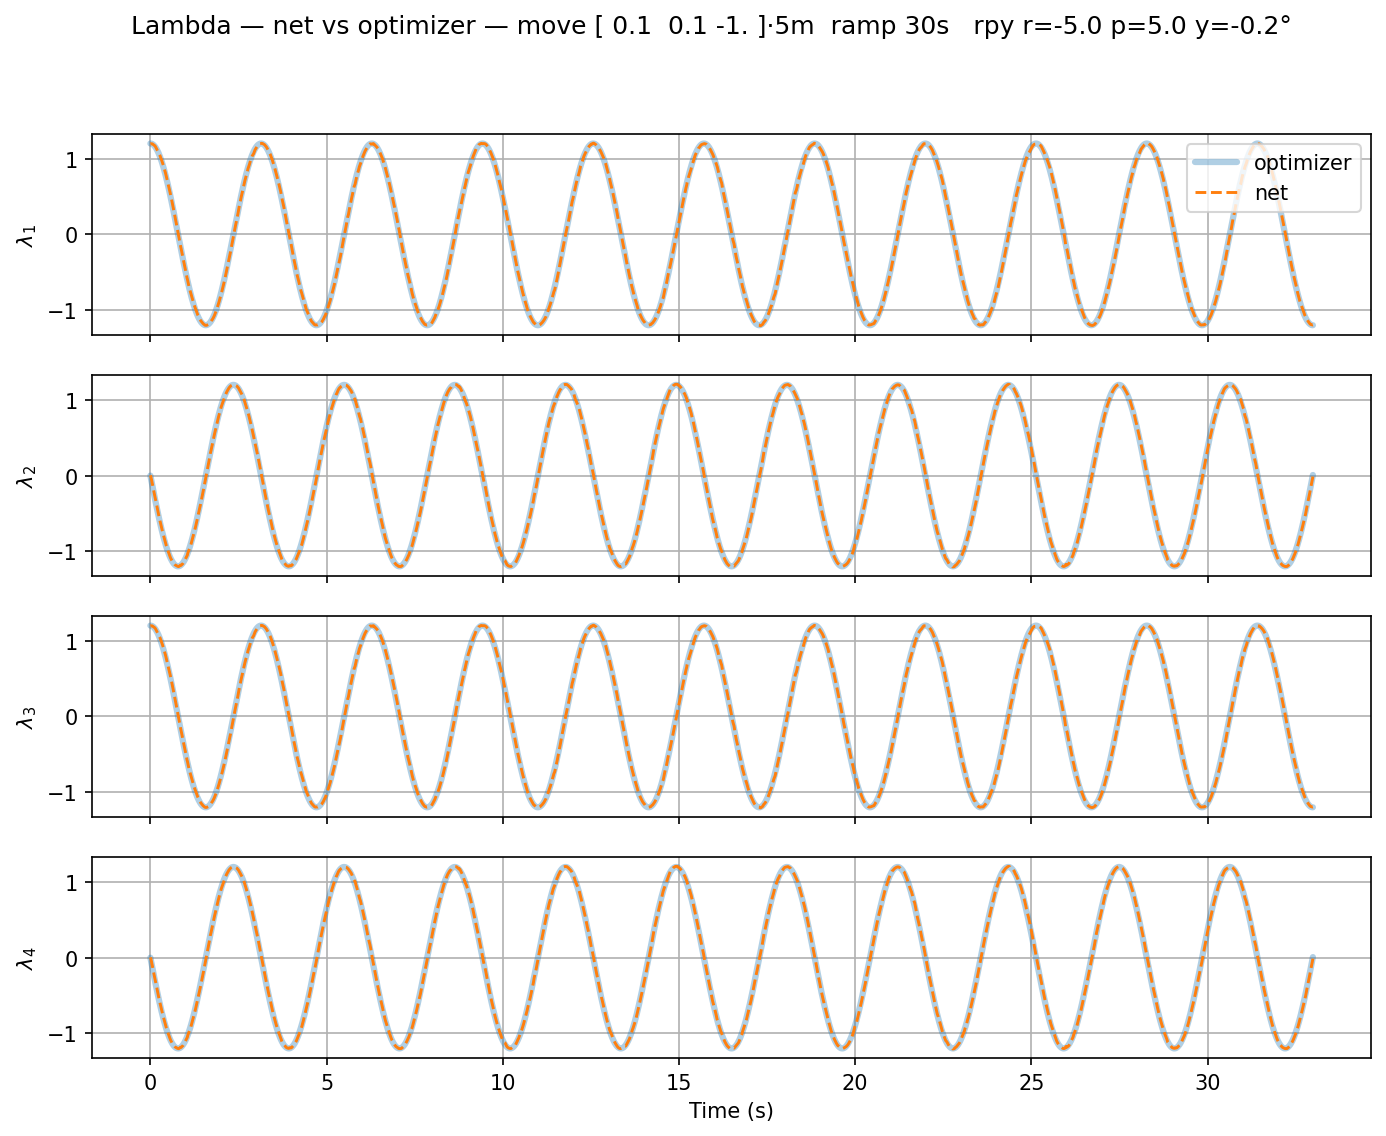
\includegraphics[width=0.8\textwidth]{figures/fig-gen-dir2-lambda.png}
  \caption{$\lambda$ produced by the network vs.\ the optimizer.}
  \label{fig:gen-dir2-lambda}
\end{figure}

\begin{figure}[H]
  \centering
  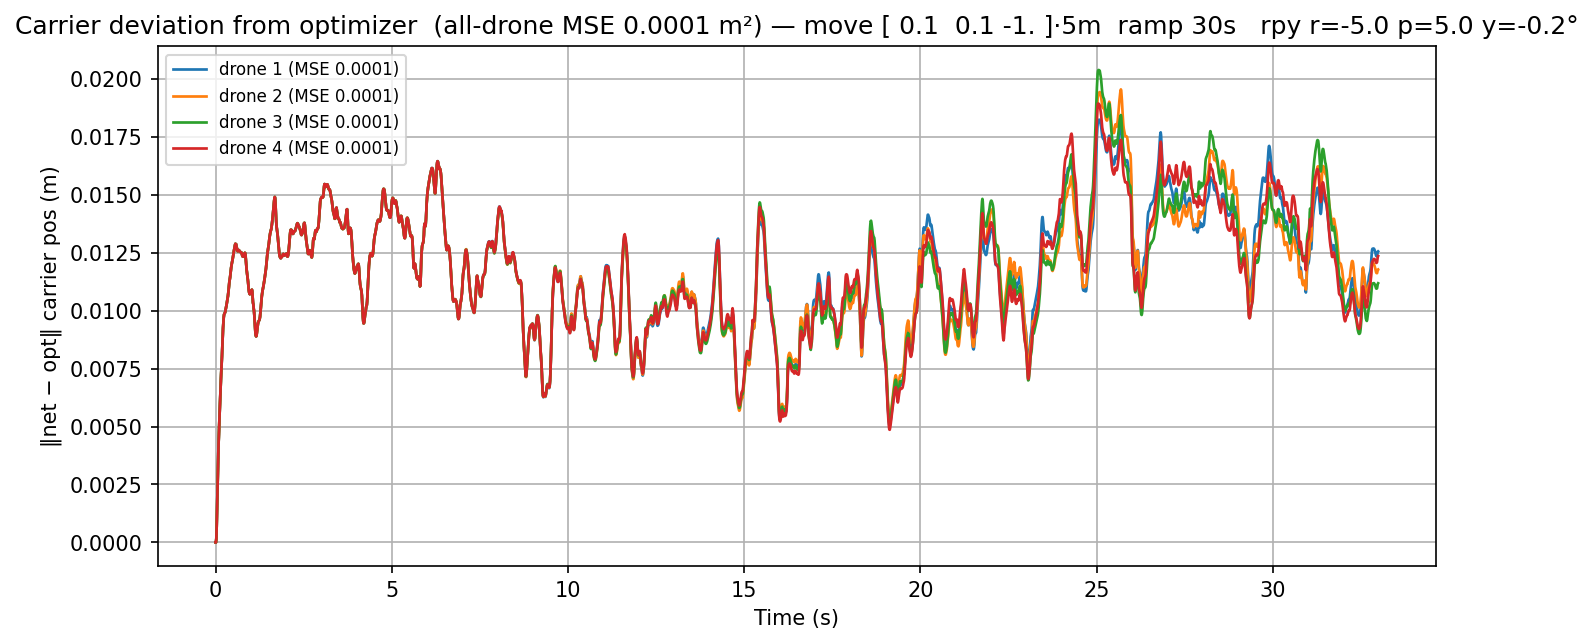
\includegraphics[width=0.8\textwidth]{figures/fig-gen-dir2-carrier-dev.png}
  \caption{Carrier deviation from the optimizer.}
  \label{fig:gen-dir2-carrier-dev}
\end{figure}

\begin{figure}[H]
  \centering
  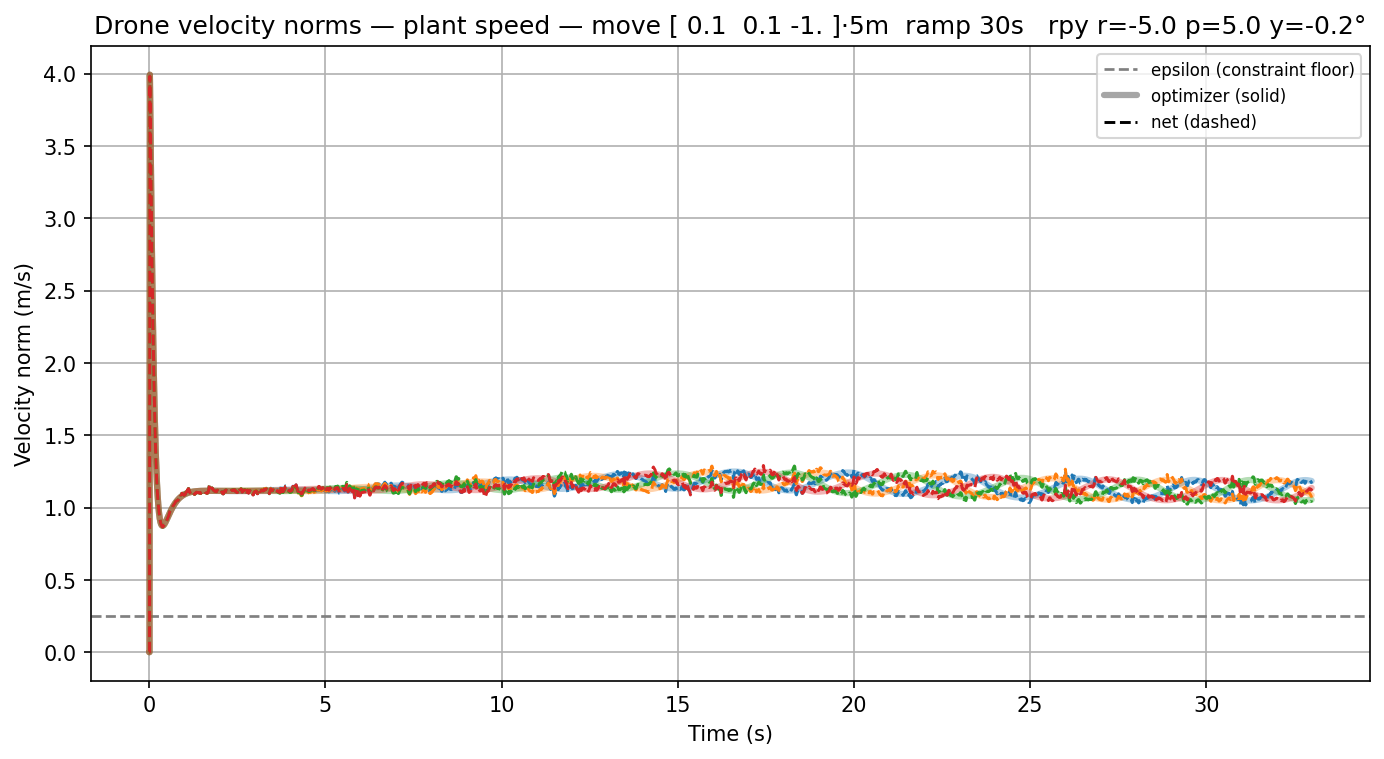
\includegraphics[width=0.8\textwidth]{figures/fig-gen-dir2-vnorms.png}
  \caption{Drone velocity norms (plant speed).}
  \label{fig:gen-dir2-vnorms}
\end{figure}

\begin{figure}[H]
  \centering
  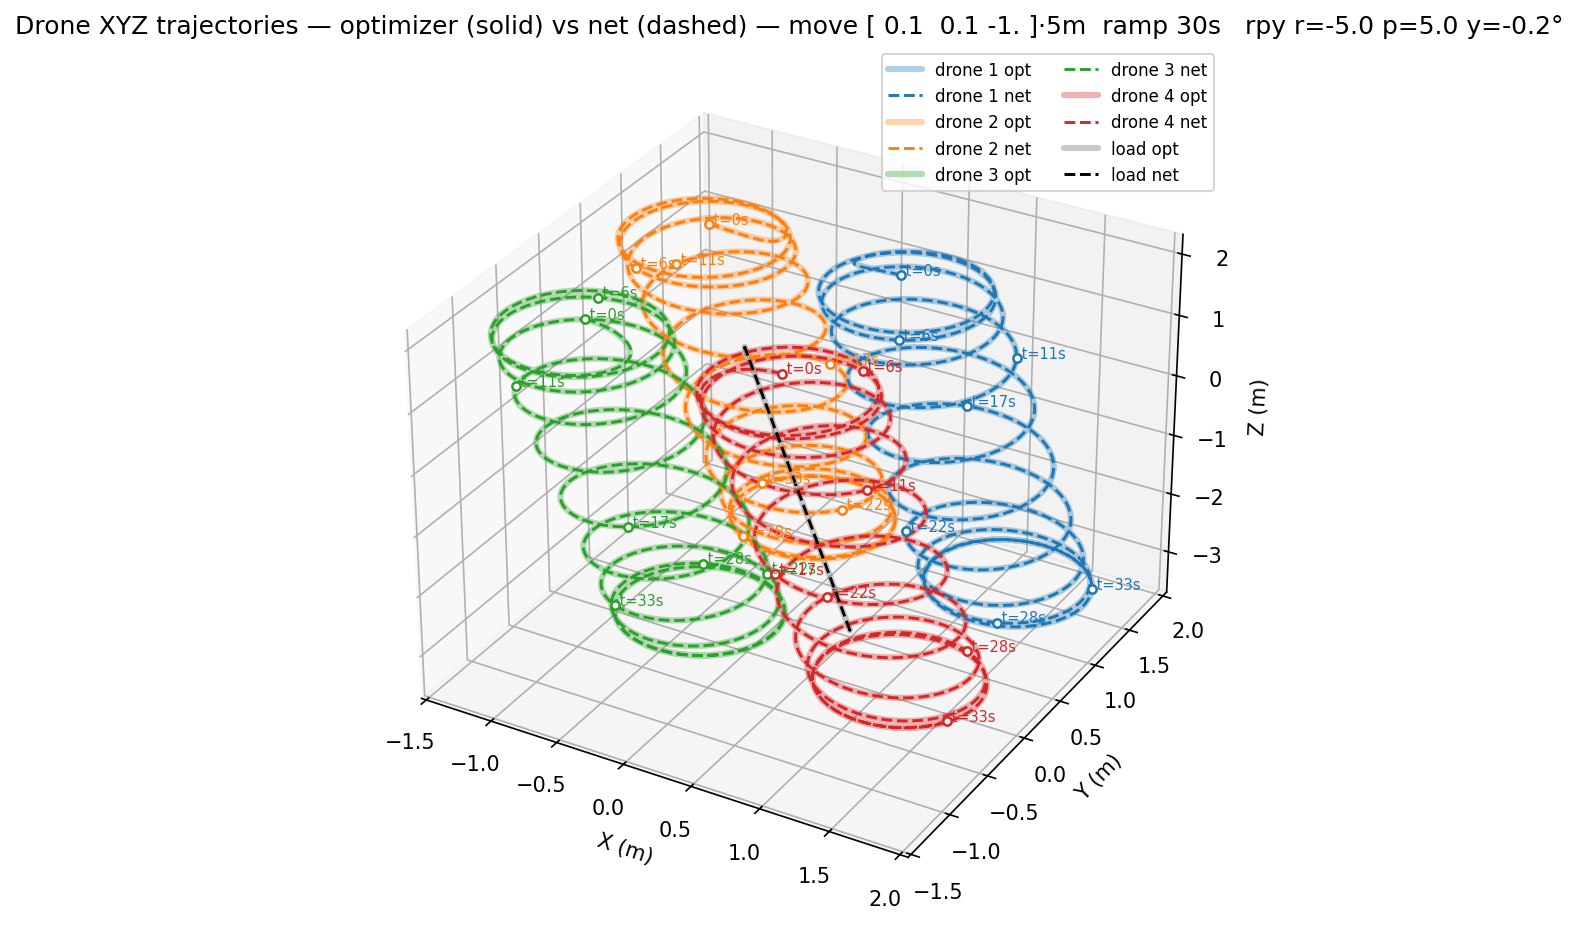
\includegraphics[width=0.8\textwidth]{figures/fig-gen-dir2-xyz.png}
  \caption{Drone XYZ trajectories: optimizer (solid) vs.\ net (dashed).}
  \label{fig:gen-dir2-xyz}
\end{figure}

\begin{table}[H]
  \centering
  \caption{Performance of the network on generalization direction 2.}
  \label{tab:gen-dir2}
  \begin{tabular}{lcc}
    \hline
    \textbf{Metric} & \textbf{Network} & \textbf{Optimizer} \\
    \hline
    Load tracking MSE (m$^2$) & 0.00035 & 0.00035 \\
    Load tracking max error (m) & 0.02697 & 0.02697 \\
    \hline
    \multicolumn{3}{l}{\textbf{Carrier deviation from optimizer, MSE (m$^2$)}} \\
    \hline
    Drone 1 & 0.00014 & -- \\
    Drone 2 & 0.00015 & -- \\
    Drone 3 & 0.00015 & -- \\
    Drone 4 & 0.00015 & -- \\
    All drones & 0.00015 & -- \\
    \hline
    \multicolumn{3}{l}{\textbf{$\lambda$ deviation from optimizer, MSE}} \\
    \hline
    Drone 1 & 0.00034 & -- \\
    Drone 2 & 0.00038 & -- \\
    Drone 3 & 0.00034 & -- \\
    Drone 4 & 0.00038 & -- \\
    All drones & 0.00036 & -- \\
    \hline
  \end{tabular}
\end{table}

\noindent\textbf{Summary across generalization trajectories}

\begin{table}[H]
  \centering
  \caption{Average network performance across all five generalization trajectories (longer-time, shorter-time, larger-magnitude, direction 1, direction 2).}
  \label{tab:gen-summary}
  \begin{tabular}{lc}
    \hline
    \textbf{Metric} & \textbf{Average (all drones)} \\
    \hline
    Carrier deviation from optimizer, MSE (m$^2$) & 0.00014 \\
    $\lambda$ deviation from optimizer, MSE & 0.00036 \\
    \hline
  \end{tabular}
\end{table}

\section{Phase Two : Reinforcement Learning}

\subsection{Single trajectory}

\subsection{Analysis of failure modes}

\subsection{Generalization}

\subsubsection{Generalization across time}

\subsubsection{Generalization across distances}

\subsubsection{Generalization across directions}

\subsubsection{History-Augmented Observation Space}

\subsubsection{Centralized Controller Policy Guidance experiment (using Supervised Learning)}

\subsubsection{Behavior Cloning (BC) of multiple policies}
